%----------------------------------------------------------------------------------------
%	Capítulo 5
%----------------------------------------------------------------------------------------

\pagestyle{myportland}
%\pagenumbering{arabic}
\doublespacing
\chapter[----- Diseño mecatrónico integral]{Diseño mecatrónico integral}
\thispagestyle{myportland}

%%%%%%%%%%%%%%%%%%%%%%%%%%%%%%%%%%%%%%%%%%%%%%%%%%%%%%%%%%%%%%
%%%%%                                                    %%%%%
%%%%%             DISEÑO MECATRÓNICO EN SÍ               %%%%%
%%%%%                                                    %%%%%
%%%%%%%%%%%%%%%%%%%%%%%%%%%%%%%%%%%%%%%%%%%%%%%%%%%%%%%%%%%%%%

%% NUEVA SECCIÓN X.X
\section{Desarrollo de diseño mecatrónico integral}
\label{sec:desarrollo de diseno mecatronico integral}

En la sección llamada \textit{"Desarrollo del diseño mecatrónico conceptual"} \footnote{\cite{DiazVergara2020}} se analizó el concepto de solución óptimo. En la Figura \ref{fig:estado diseno mecatronico etapa 3} se muestra la etapa final de unir las sub-soluciones para desarrollar una forma viable de implementarlos de una forma integral.

\begin{myfigure}[H]
	\centering
	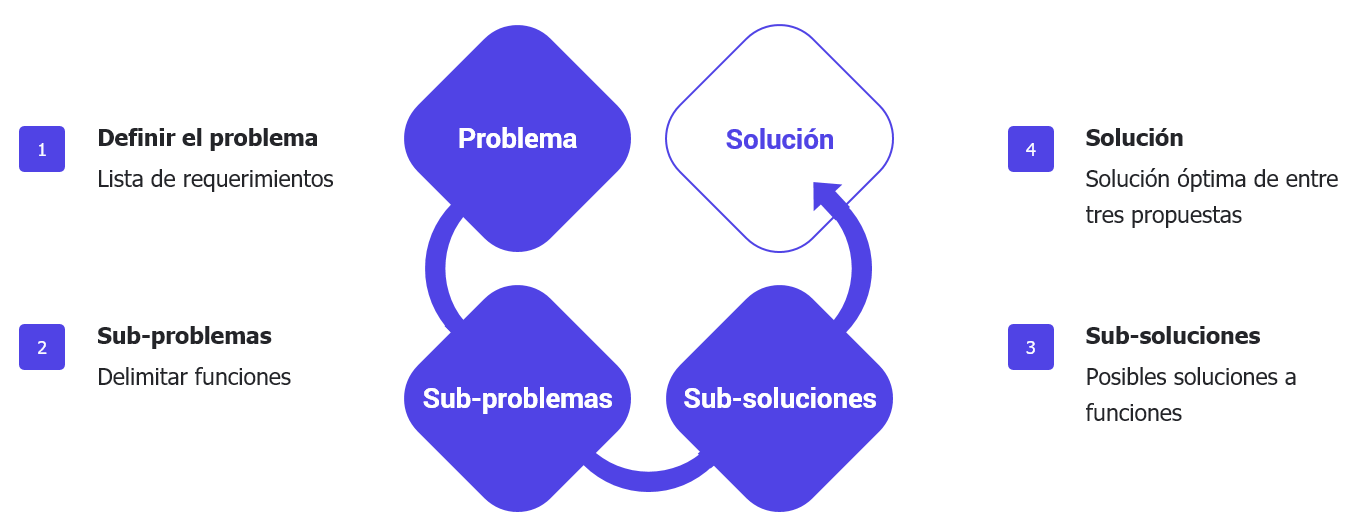
\includegraphics[width=1\textwidth]{chapter5/estado diseno subsoluciones.png}
	\caption{Estado de diseño mecatrónico: sub-soluciones}
	\begin{myflushleftportland}
		Fuente: Elaboración propia
	\end{myflushleftportland}
	\label{fig:estado diseno mecatronico etapa 3}
\end{myfigure}

Según el proceso de diseño indicado en la norma VDI 2221 que se muestra en la Figura \ref{fig:vdi2221} se parte del diseño conceptual propuesto (5) y se presenta el diseño integral (6)\footnote{\cite{Pahl2007}}, también llamado diseño de ingeniería, que abarca diferentes puntos: dimensionamiento del sistema; cálculos; selección técnica de materiales entorno a su aplicación; selección técnica de sensores; actuadores y dispositivos de control; lógica del control del sistema y su estrategia; planos mecánicos: ensamble y despiece; planos eléctricos y/o electrónicos; simulaciones de la máquina y una estimación de costos.

\begin{myfigure}[H]
	\centering
	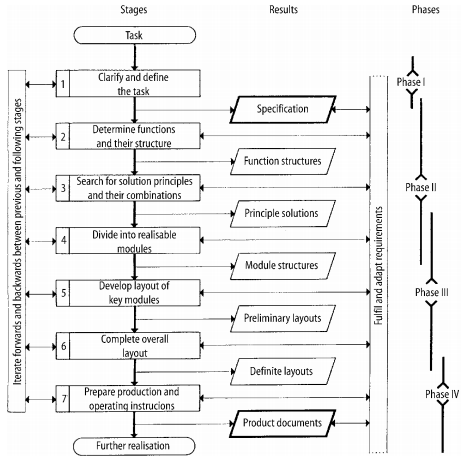
\includegraphics[width=0.75\textwidth]{chapter5/vdi2221.png}
	\caption{Fases de diseño según VDI 2221}
	\begin{myflushleftportland}
		Fuente: \cite{Pahl2007}
	\end{myflushleftportland}
	\label{fig:vdi2221}
\end{myfigure}



%% NUEVA SECCIÓN X.X.X
\subsection{Descripción del sistema integral}
\label{ssec:descripcion del sistema integral}

Respecto al diseño conceptual, existen algunas modificaciones en los tipos de dispositivos por características técnicas detectadas en el desarrollo de ingeniería del sistema: el cambio del servomotor por un mecanismo de motor a pasos con leva-seguidor que disminuye el desgaste por el sentido de giro; la batería ya no es parte del sistema, el operario debe suministrar la energía necesaria; el adicional de una cámara para el seguimiento de la trayectoria de truchas en el mecanismo de distribución; la variación de el uso de un microcontrolador a microprocesador debido a la potencia computacional requerida; el cambio de bombas sumergibles a bombas de agua por la eficiencia y potencia necesaria en el proyecto\footnote{El precio de las bombas sumergibles sube considerablemente correspondiente a la potencia requerida.}; remoción de la reja al inicio accionada por un motor debido al coste de implementación y reemplazo con un tapón de plástico.

La máquina clasificadora y contadora de truchas\footnote{CCT}, y su sistema respectivo tienen como función principal recepcionar truchas mediante una tolva, procesar la clasificación, conteo y distribución hacia tres jaulas flotantes en medio de la Laguna de Paucarcocha.\footnote{\cite{DiazVergara2020}} La máquina se sitúa sobre el agua y es empleada por un operario, que se encarga de extraer truchas con una sacadera telescópica\footnote{También llamada cal-cal.}. En las siguientes páginas se analizan dos puntos generales concernientes al sistema: arquitectura de hardware y la selección de materiales de fabricación por subsistema.

%\textcolor{blue}{[BORRADOR] Explicar cambios importantes respecto a Diseño conceptual sustentando cálculos realizados o algoritmo. Cambios realizados: servomotor -> Leva + Motor a pasos; batería ya no es requerida, el operario se ocupa de suministrar batería; cámara simple agregada mediante stickers de puntos rojos, solo analizamos color rojo de compuertas y filtrar a la trucha. Ya no se realiza diagrama eléctrico, todo será manejo de DC. Potencia computacional requerida aumenta de microcontrolador a microprocesador [/BORRADOR]}\\

%% NUEVO SUBSECCION X.X.X.X
\subsubsection{Arquitectura de hardware}

En la Figura \ref{fig:arquitectura de hardware del sistema} se muestra la propuesta de arquitectura de hardware. Esta arquitectura muestra las entradas de energía del sistema, su redistribución a cada componente, el control asociado a cada pieza mediante el subsistema de control y los protocolos o energía asociado a cada par de bloques. Además, el tipo de conexión se detalla en la leyenda. 

\begin{myfigure}[H]
	\centering
	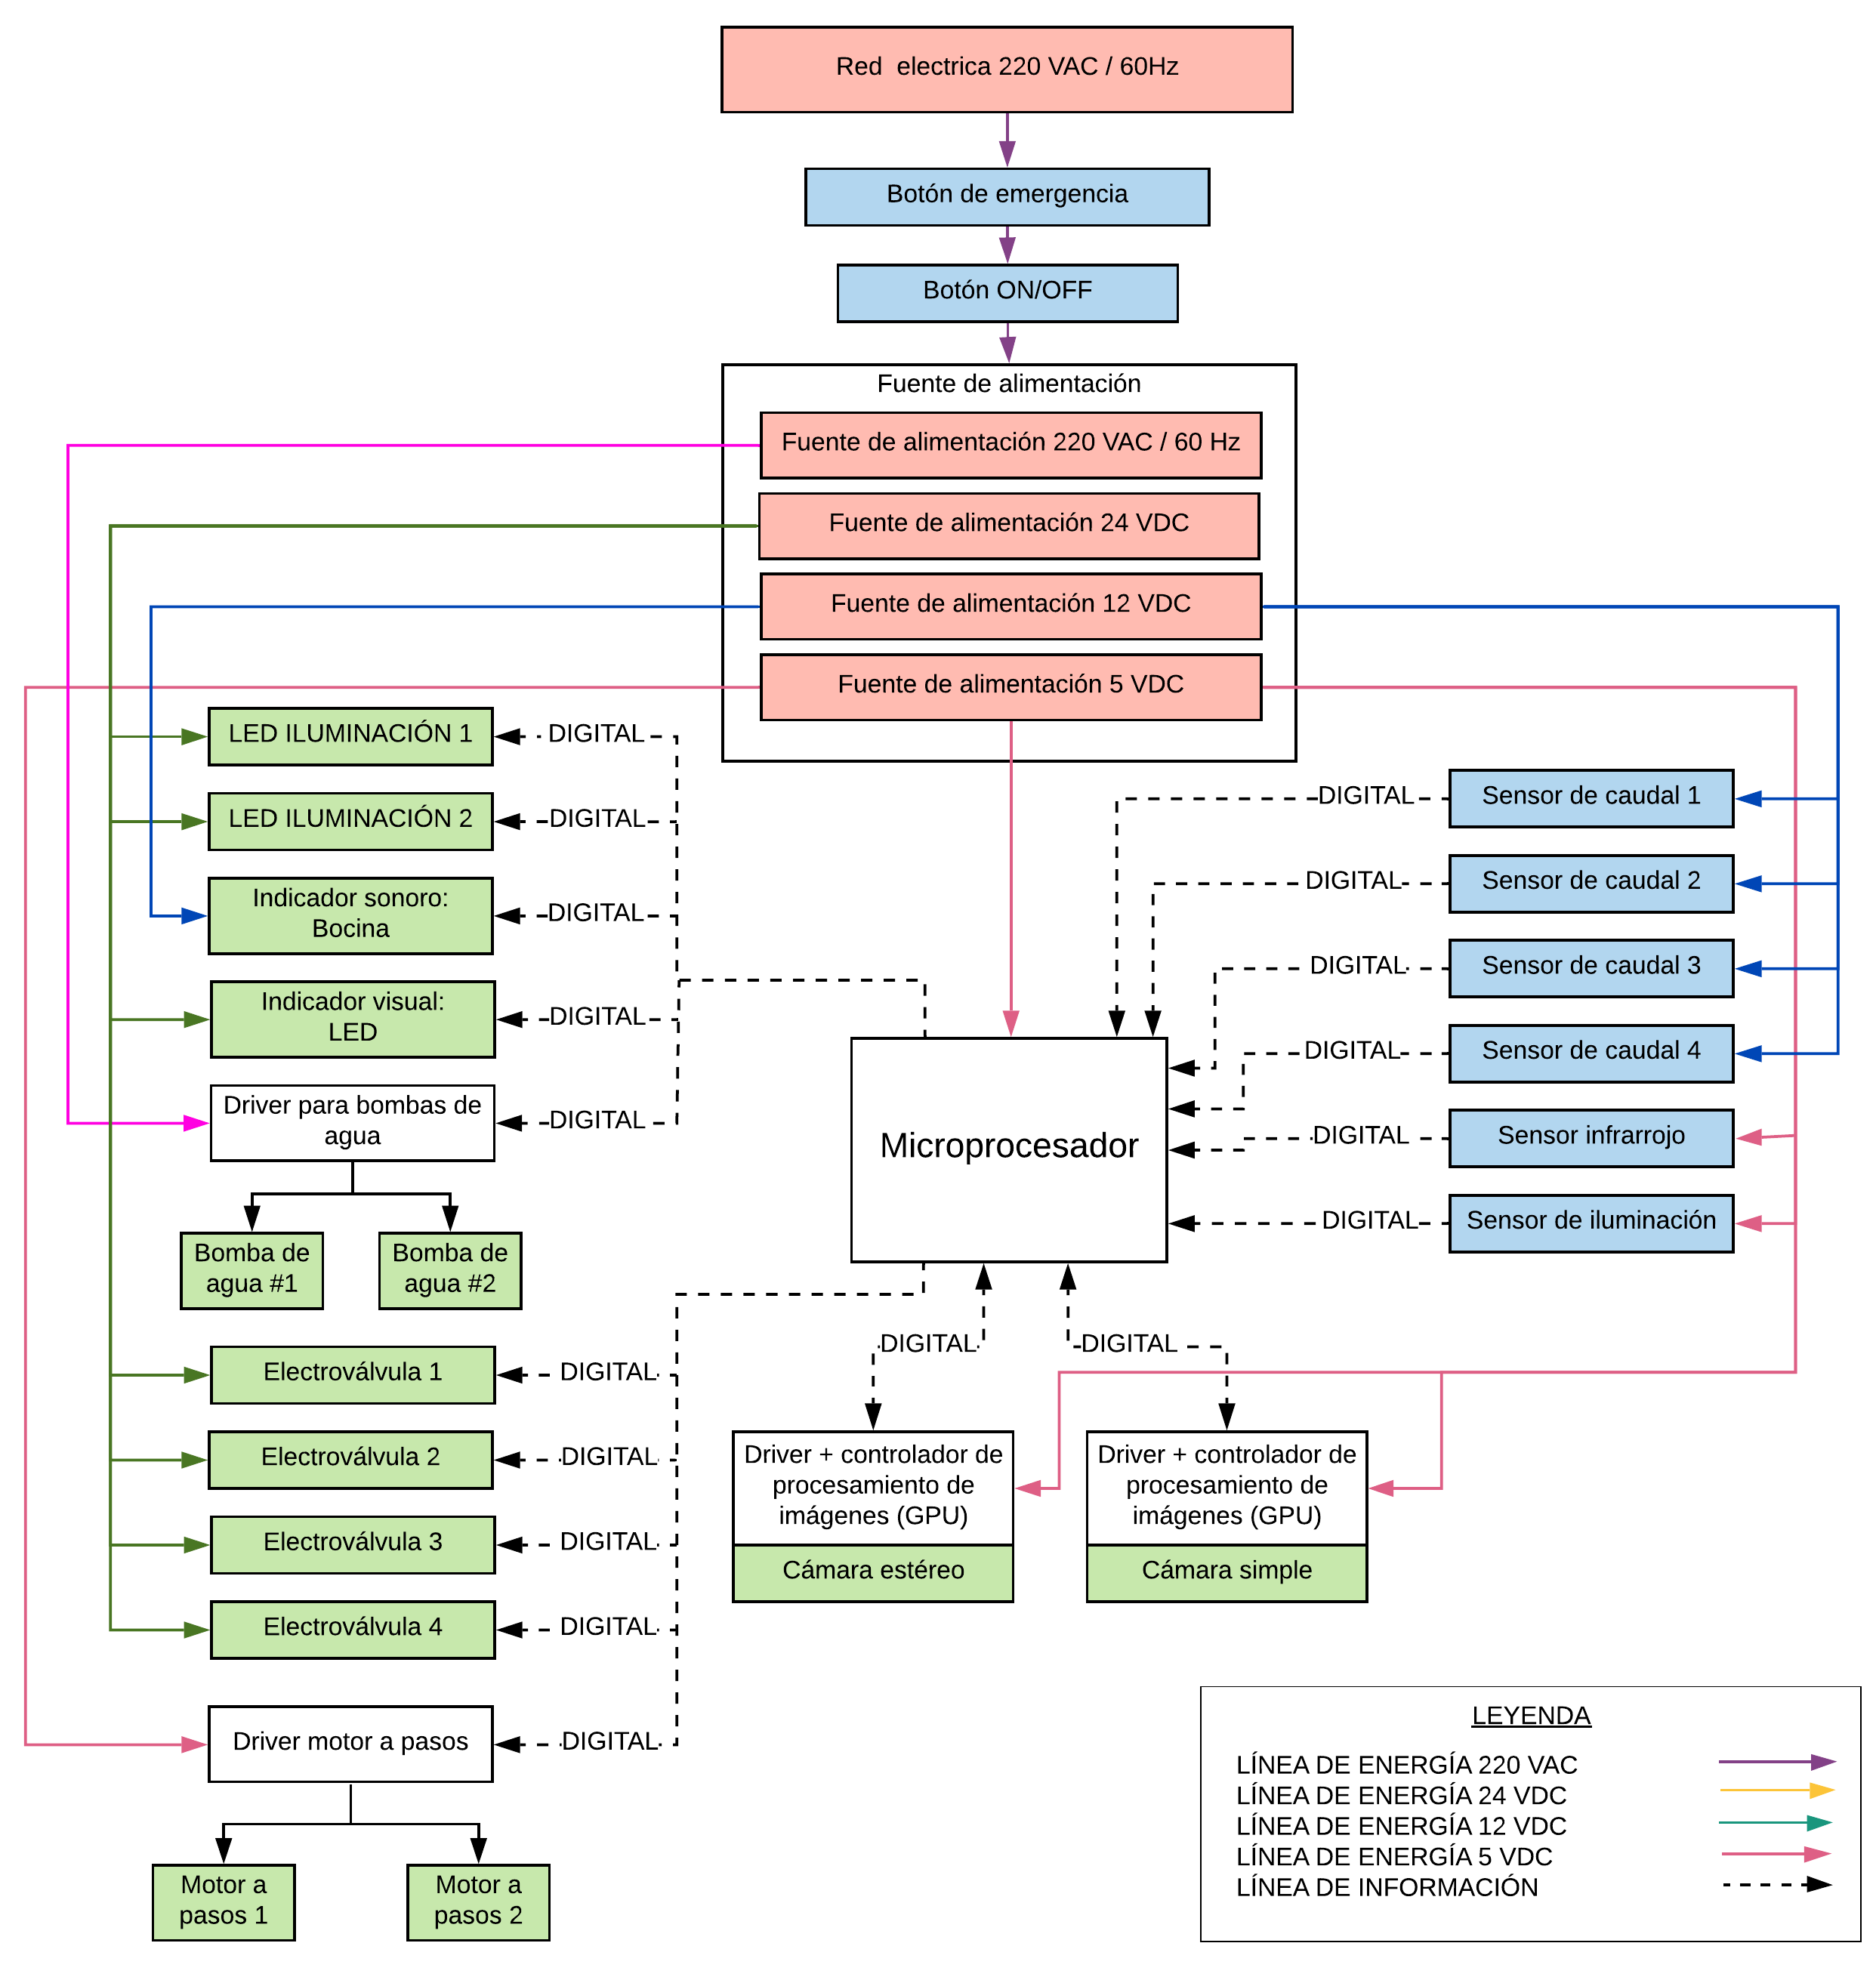
\includegraphics[width=1\textwidth]{chapter5/arquitectura de hardware del sistema.png}
	\caption{Arquitectura de hardware del sistema}
	\begin{myflushleftportland}
		Fuente: Elaboración propia.
	\end{myflushleftportland}
	\label{fig:arquitectura de hardware del sistema}
\end{myfigure}

%\textcolor{blue}{[BORRADOR] Terminar de definir los voltajes que se utilizarán. [/BORRADOR]}

%% NUEVO SUBSECCION X.X.X.X
\subsubsection{Selección de materiales de fabricación}
\label{sssec:seleccion de materiales de fabricacion}

Cada subsistema posee mecanismos que se rigen por un material en general, esto incluye a las partes principales del subsistema. Sin embargo, no considera el material de tornillos, ajustes o dispositivos similares. Existen así mismos requisitos que se pueden generalizar para todos los subsistemas por el entorno de trabajo a la que estará sometida la máquina detallados en la \textit{"Lista de requerimientos"} \footnote{\cite{DiazVergara2020}.}. Basado en dichas demandas, cada subsistema es analizado y presentado con dos alternativas posibles de materiales. Consecuentemente, se elige un material decisivo para ser empleado bajo el sustento técnico que se explicará en los siguientes párrafos.

\begin{itemize}
	\item \textbf{Subsistema de recepción y traslado de truchas:} Cuenta con dos mecanismos; recepción de truchas y tuberías de traslado. El primero debe recepcionar a las truchas y dirigirlas al mecanismo de tuberías. El segundo debe trasladar a las truchas de un punto a otro de la máquina mediante las tuberías. En la Tabla \ref{tab:tabla comparativa de propiedades entre aluminio vs acero inoxidable} se comparan técnicamente las propiedades mecánicas, térmicas y ópticas de dos materiales.
	
	\begin{mytable}[H]
		\centering
		\caption{Tabla comparativa de propiedades entre $Aluminio$ vs $Acero \quad Inoxidable$}
		\label{tab:tabla comparativa de propiedades entre aluminio vs acero inoxidable}
		\begin{tabular}{|l|c|c|}
			\hline
			\multicolumn{1}{|c|}{\textbf{Propiedad}} & \textbf{Aluminio} & \textbf{Acero Inoxidable} \\ \hline
			Módulo de Young ($GPa$) & 69 & 200 \\ \hline
			Esfuerzo de fatiga $Y$ ($MPa$) & 58-110 & 210-440 \\ \hline
			Resistencia a la tracción ($MPa$) & 130-410 & 580-1180 \\ \hline
			Temperatura máxima mecánica (°$C$) & 650 & 1450 \\ \hline
			Conductividad térmica ($W/m-K$) & 170 & 16 \\ \hline
			Expansión térmica (${\mu}m/m-K$) & 24 & 17 \\ \hline
			Conductividad eléctrica ($\%$) & 43 & 2.4 \\ \hline
			Densidad ($g/cm^3$) & 2.7 & 7.8 \\ \hline
		\end{tabular}
		\begin{flushleft}
			*Terminología técnica de los materiales: Aluminio 6061, Acero Inoxidable ANSI 304.\\		
			Fuente: \cite{MakeItFrom2020}.
		\end{flushleft}
	\end{mytable}

	El material escogido es Aluminio 6061 por tener una densidad menor, facilidad de realizar juntas de soldadura, y aunque tenga menor resistencia mecánica cumple con los requerimientos mínimos asociados al subsistema mencionado.
	
	\item \textbf{Subsistema de procesamiento de imágenes:} Cuenta con los mecanismos de tuberías y juego de espejos. El primero debe brindar a la cámara suficiente transparencia para obtener una fotografía adecuada. El segundo debe brindar a la cámara más perfiles del cuerpo que es trasladado por la tubería. En la Tabla \ref{tab:tabla comparativa de propiedades entre pmma vs pvdf vs petg} se compara técnicamente las propiedades mecánicas, térmicas y ópticas de tres materiales.
	
	\begin{mytable}[H]
		\centering
		\caption{Tabla comparativa de propiedades entre $PMMA$, $PVDF$ y $PETG$}
		\label{tab:tabla comparativa de propiedades entre pmma vs pvdf vs petg}
		\begin{tabular}{|l|c|c|c|}
			\hline
			\multicolumn{1}{|c|}{\textbf{Propiedad}} & \multicolumn{1}{c|}{\textbf{PMMA}} & \textbf{PVDF}& \textbf{PETG} \\ \hline
			Resistencia al impacto: con muescas ($J/m$) & 74 & 180 & 77  \\ \hline
			Expansión térmica (${\mu}m/m-K$)  & 76 & 120 & 68 \\ \hline
			Densidad ($g/cm^3$) & 1.2 & 1.8  & 1.3 \\ \hline
			Resistencia al peso  & 32 & 20 & 25 \\ \hline
			Alargamiento a la rotura ($ \% $) & 4 & 49 & 53 \\ \hline
			Incidencia de luz trasmitida ($ \% $) & 92 & - & - \\ \hline
			Índice de refracción & 1.5 & 1.4 & 1.6\\ \hline			
		\end{tabular}
		\begin{flushleft}
			*Terminología técnica de los materiales: Polimetilmetacrilato (Acrílico)(PMMA), Fluoruro de polivinilideno (PVDF), Tereftalato de polietileno modificado con glicol (PETG).\\		
			Fuente: \cite{Brydson1999,Berins1991,Harper2000,MakeItFrom2020}.
		\end{flushleft}
	\end{mytable}

	Tanto el PMMA como el PETG tienen menores propiedades mecánicas que PVDF, pero en cuanto a densidad los materiales mencionados son más livianos comparados con el PVDF. En cuanto a las propiedades ópticas, el PMMA tiene un índice de refracción mayor que el PVDF pero menor que el PETG. Sin embargo, la el PMMA es el material más usado en propósitos ópticos comparado con los otros materiales mencionados. El PMMA transparente se puede encontrar en el mercado nacional e internacional por lo que se opta por este material para el subsistema mencionado. En el caso del juego de espejos, las propiedades ópticas son primordiales, por lo que se escoge PMMA.
	
	\item \textbf{Subsistema de procesamiento de suministro de energía y subsistema de control e interacción con el usuario:} Los materiales son propios de los dispositivos electrónicos comerciales dependientes de la tecnología que se selecciona, por lo que se omite una clasificación de materiales en estos subsistemas.
	
	%\item \textbf{:} Los materiales son propios de los dispositivos que serán adquiridos.
	
	\item \textbf{Subsistema de flotación:} Cuenta con dos mecanismos; armadura y flotadores. El primero debe funcionar como esqueleto para los otros subsistemas y del mismo. El segundo debe mantener el sistema a flote. En la Tabla \ref{tab:tabla comparativa de propiedades entre hdpe vs pvcu} se compara técnicamente las propiedades mecánicas, térmicas y ópticas de dos materiales.
	
	\begin{mytable}[H]
		\centering
		\caption{Tabla comparativa de propiedades entre $HDPE$ vs $PVC-U$}
		\label{tab:tabla comparativa de propiedades entre hdpe vs pvcu}
		\begin{tabular}{|l|c|c|}
			\hline
			\multicolumn{1}{|c|}{\textbf{Propiedad}} & \textbf{HDPE} & \textbf{PVC-U} \\ \hline
			Densidad ($g/cm^3$) & 1.0-1.3 & 1.4 \\ \hline
			Elongación a rotura ($\%$) & 2.5-100 & 58 \\ \hline
			Resistencia al impacto ($J/m$) & 50-260 & 360 \\ \hline
			Resistencia al peso: Flexión & 19-32 & 20 \\ \hline
			Resistencia a la tracción ($MPa$) & 24-80 & 47 \\ \hline
		\end{tabular}
		\begin{flushleft}
			*Terminología técnica de los materiales: Polietileno de alta densidad (HDPE), Cloruro de polivinilo no plastificado (Rígido) (uPVC, PVC-U)\\		
			Fuente: \cite{Brydson1999,Berins1991,Harper2000,MakeItFrom2020}.
		\end{flushleft}
	\end{mytable}
	
	En los flotadores es crucial las propiedades mecánicas, ya que en caso de falla puede hundir todo el sistema. La búsqueda de un material con baja densidad, alta resistencia a la tracción, impacto y al peso determinan el material escogido como HDPE. Además dicho material es comercializado nacionalmente e internacionalmente. De forma similar, la armadura debe poseer buenas propiedades mecánicas y por eso se selecciona Acero Inoxidable.
	
\end{itemize}

Finalmente, en las Tablas \ref{tab:tabla comparativa de propiedades entre aluminio vs acero inoxidable}, \ref{tab:tabla comparativa de propiedades entre pmma vs pvdf vs petg} y \ref{tab:tabla comparativa de propiedades entre hdpe vs pvcu} se comparan diversos materiales para el correspondiente subsistema. Los materiales de fabricación finales para cada subsistema se muestran en la Tabla \ref{tab:materiales de fabricacion por subsistema}, fueron seleccionados por su superioridad en las propiedades técnicas que son valoradas en este proyecto. 

\begin{savenotes}
	\begin{mytable}[H]
		\centering
		\caption{Materiales de fabricación por subsistema}
		\label{tab:materiales de fabricacion por subsistema}
		\begin{tabular}{|l|c|c|}
			\hline
			\multicolumn{1}{|c|}{\textbf{Subsistema}} & \multicolumn{1}{c|}{\textbf{Mecanismo}} & \textbf{Material} \\ \hline
			Recepción y traslado de truchas      & Recepción de truchas   & Aluminio  \\ \hline
			Recepción y traslado de truchas      & Tuberías de traslado   & PVC-U    \\ \hline
			Procesamiento de imágenes            & Tubería                & PMMA  \\ \hline
			Procesamiento de imágenes            & Juego de espejos       & PMMA  \\ \hline
			Suministro de energía                & \multicolumn{1}{c|}{-} & -    \\ \hline
			Control e interacción con el usuario & \multicolumn{1}{c|}{-} & -  \\ \hline
			Flotación                            & Armadura               & Acero Inoxidable \\ \hline
			Flotación                            & Flotadores             & HDPE  \\ \hline
		\end{tabular}
		\begin{flushleft}
		*Terminología técnica de los materiales: Cloruro de polivinilo no plastificado (Rígido) (uPVC, PVC-U), Polimetilmetacrilato ISO 24026-1:2020\footnote{\href{https://www.iso.org/standard/77547.html}{Estándar ISO detallado}. Antecesor: 8257-1:1998. Estándar ASTM: D788-96} (Acrílico) (PMMA), Polietileno de alta densidad (HDPE), Acero Inoxidable 304, Aluminio 6061 (AL), Fluoruro de polivinilideno (PVDF).\\	
		Fuente: Elaboración propia.
		\end{flushleft}
	\end{mytable}
\end{savenotes}

%% NUEVA SECCIÓN X.X.X
\subsection{Subsistema de recepción, traslado y distribución de truchas}
\label{ssec:subsistema de recepcion, traslado y distribucion de truchas}

Este subsistema consiste en encapsular los mecanismos físicos que están en el ciclo que sigue una trucha dentro de la máquina: tolva, tuberías, bomba de agua, distribución física por mecanismos, caudales apropiados y el control respectivo. Los puntos mencionados se detallan en las siguientes páginas.

%% NUEVO SUBSECCION X.X.X.X
\subsubsection{Diseño de tolva de recepción de truchas}

El diseño implica un análisis sobre las situaciones que suceden cuando se realiza el proceso de depositar las truchas. En la Figura \ref{fig:calculo de dimensiones y angulo de la tolva} se analiza dicha situación con la finalidad de escoger un ángulo de elevación de la tolva ($\beta$) adecuado. Respecto a la tolva, se designan los siguientes valores iniciales: $A_{min},B_{min}=200 mm.$; $\beta \in [0;45] ^\circ$; ${tolva}=150 mm.$. Además, debe cumplirse que $A_{max}>B_{max}$ orientado hacia el operario que depositará la trucha.

\begin{myfigure}[H]
	\centering
	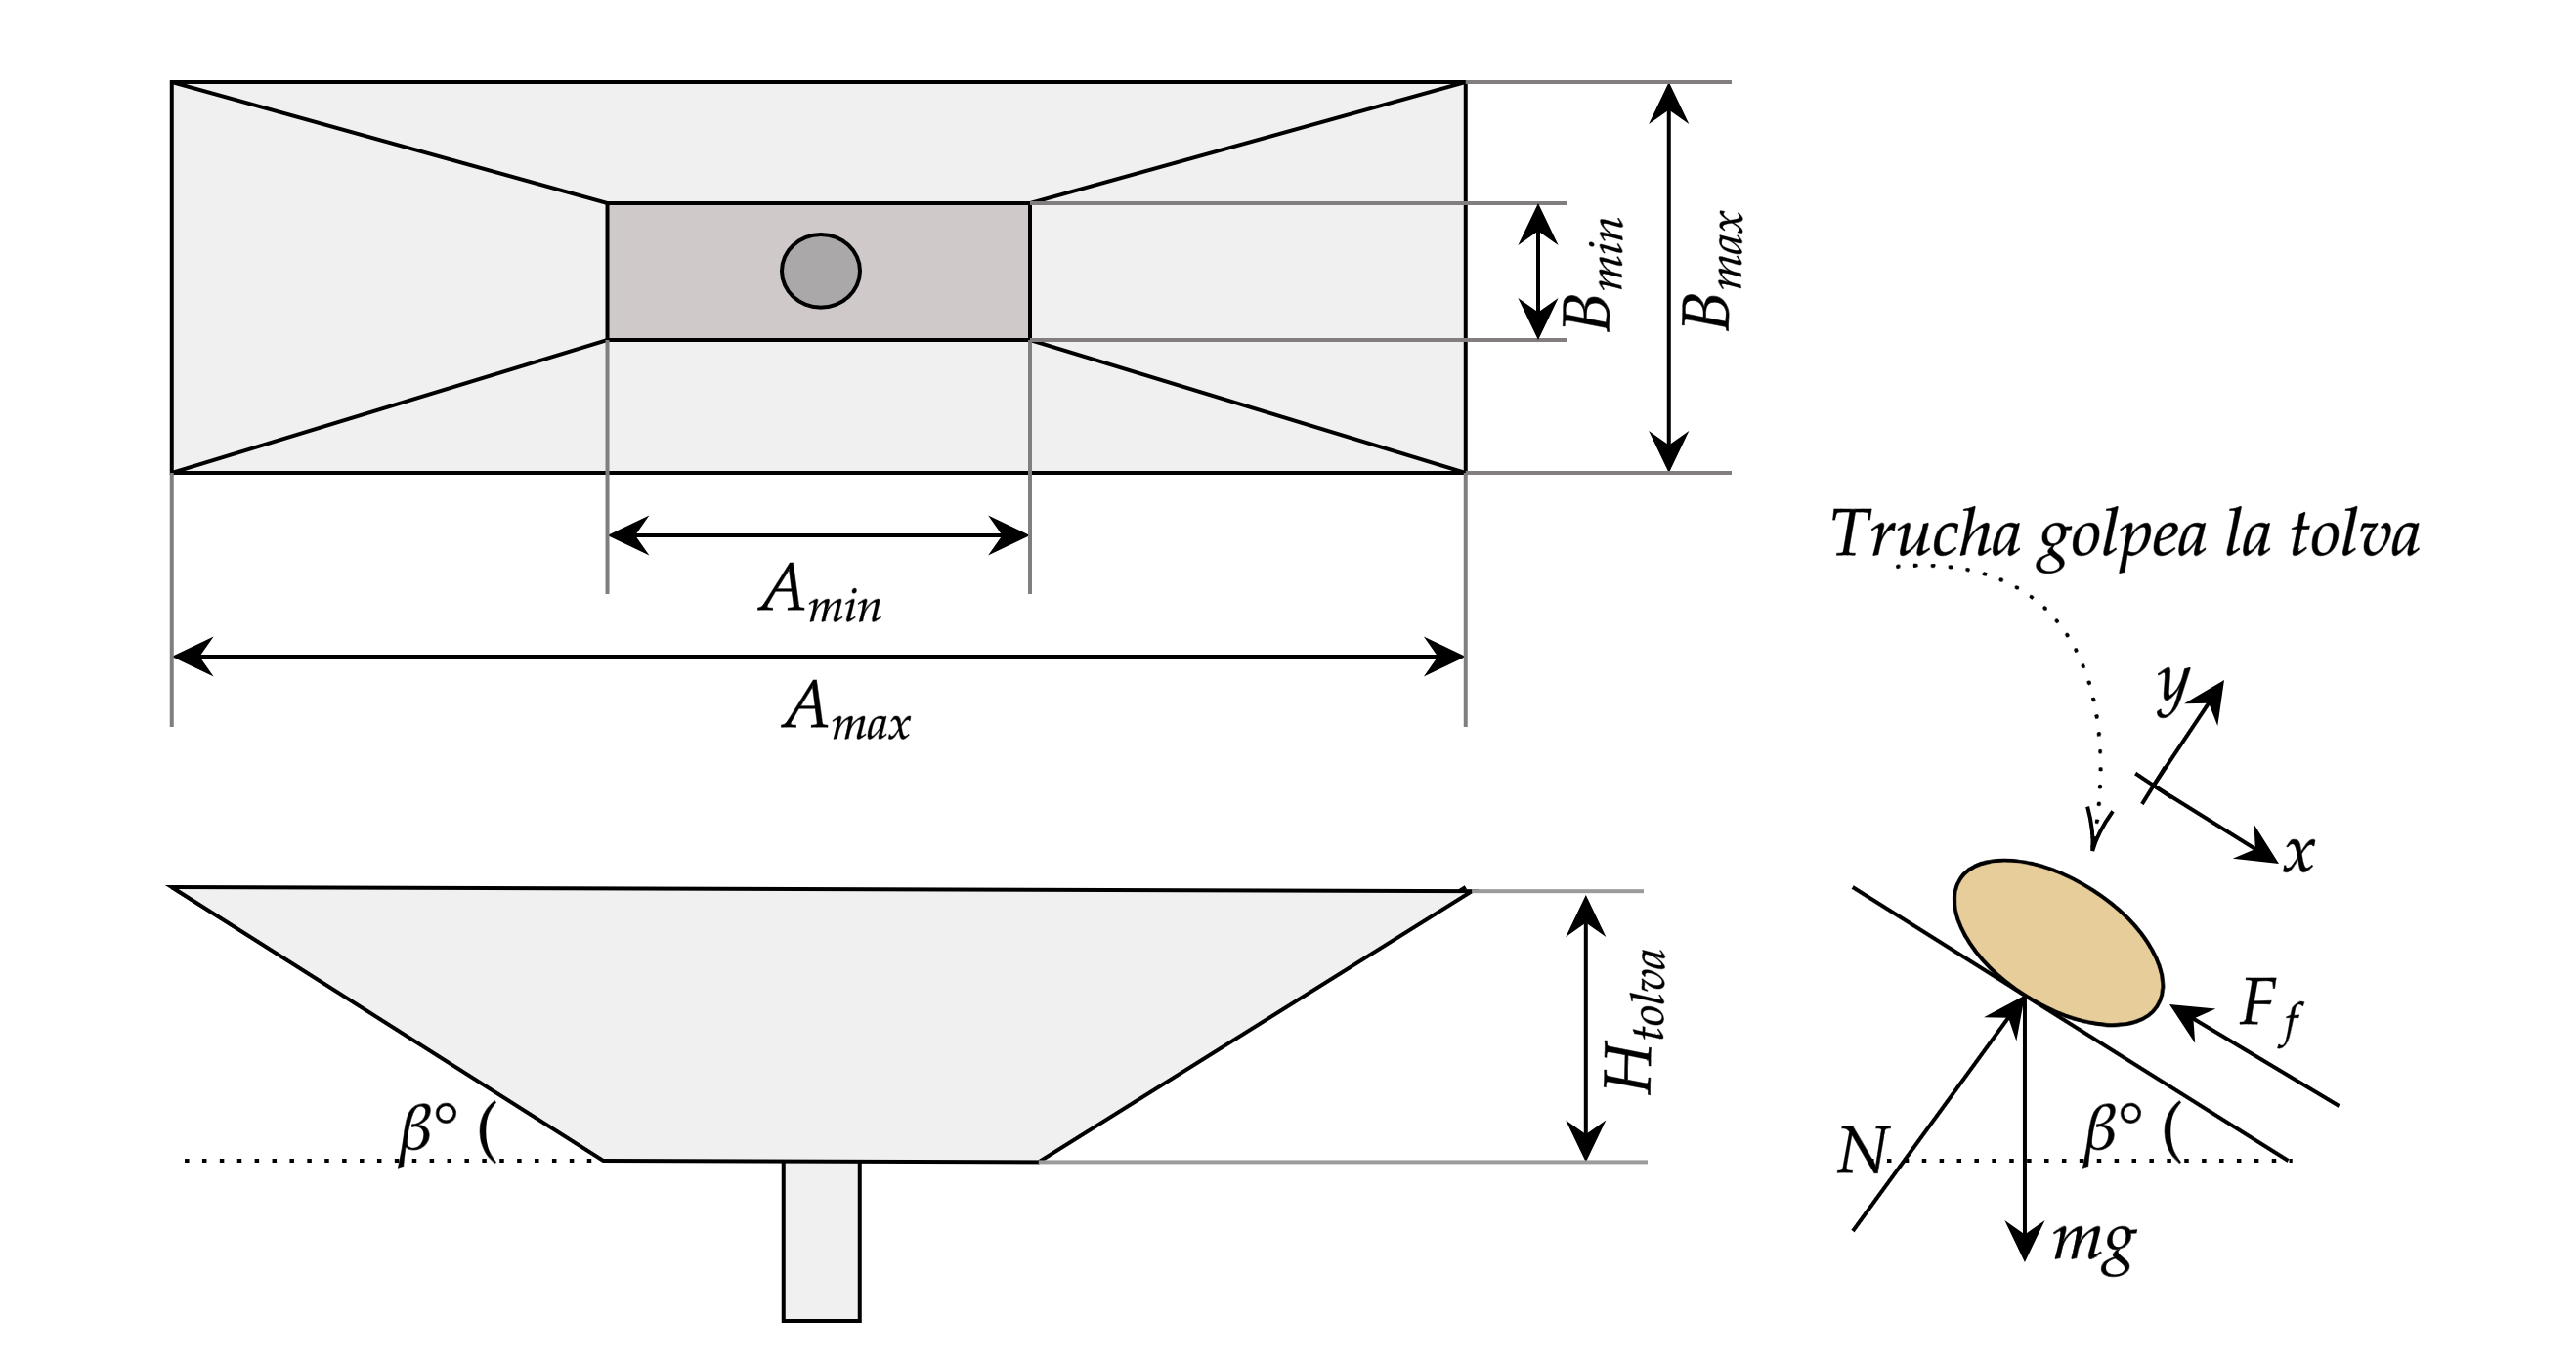
\includegraphics[width=1\textwidth]{chapter5/calculo de dimensiones y angulo de la tolva.png}
	\caption{Cálculo de dimensiones y ángulo de la tolva}
	\begin{myflushleftportland}
		Fuente: Elaboración propia.
	\end{myflushleftportland}
	\label{fig:calculo de dimensiones y angulo de la tolva}
\end{myfigure}

Parte de la Figura \ref{fig:calculo de dimensiones y angulo de la tolva} muestra el diagrama de cuerpo libre del cual se extrae la fuerza de fricción ($F_{f}$) y la fuerza normal ($N$) que se muestran en la Ecuación \ref{eq:calculo de angulo de la tolva}. Las leyes de Newton se muestran en la Ecuación \ref{eq:leyes de newton}. 

\begin{myequation}\label{eq:leyes de newton}
	\begin{split}
		F_{R}=m*a \\
		\sum_{0}^{n}F_{x,y,z}=0
	\end{split}
\end{myequation}

\begin{myequation}\label{eq:calculo de angulo de la tolva}
	\begin{split}
		F_{f}=\mu*N  \\
		\sum_{}^{}F_{y}=N-mg*cos(\beta)=0
	\end{split}
\end{myequation}

Luego, se reemplazan la Ecuación \ref{eq:calculo de angulo de la tolva} en la Ecuación \ref{eq:leyes de newton} y se obtiene la Ecuación \ref{eq:calculo de angulo de la tolva2}. La variable a despejar es la aceleración en el eje x ($\ddot{x}$).

\begin{myequation}\label{eq:calculo de angulo de la tolva2}
	\begin{split}
		mg*sin(\beta)-F_{f}&=m*\ddot{x} \\
		mg*sin(\beta)-\mu_{k}*mg*cos(\beta)&=m*\ddot{x} \\
		g*sin(\beta)-g*\mu_{k}*cos(\beta)&=\ddot{x}
	\end{split}
\end{myequation}

Para disminuir el impacto de la trucha sobre la tolva o sobre las tuberías interiores se debe disminuir la aceleración de la trucha al ser depositada en la tolva. La Figura \ref{fig:grafico angulo de tolva vs aceleracion} muestra la ecuación que relaciona la aceleración con el ángulo de elevación de la pared de la tolva. Consecuentemente, se escoge un ángulo ($\beta=30^\circ$) para tener una aceleración aproximadamente nula ($\ddot{x}\approx0$). Se considera $\mu_{k}=0.57$ para el material escogido en la sección \ref{sssec:seleccion de materiales de fabricacion}. Consecuentemente, se calculan los valores de $A_{max}\approx{900} mm.$ y $B_{max}\approx{700} mm.$, respectivamente.

% Material escogido Acero inoxidable

\begin{myfigure}[H]
	\centering
	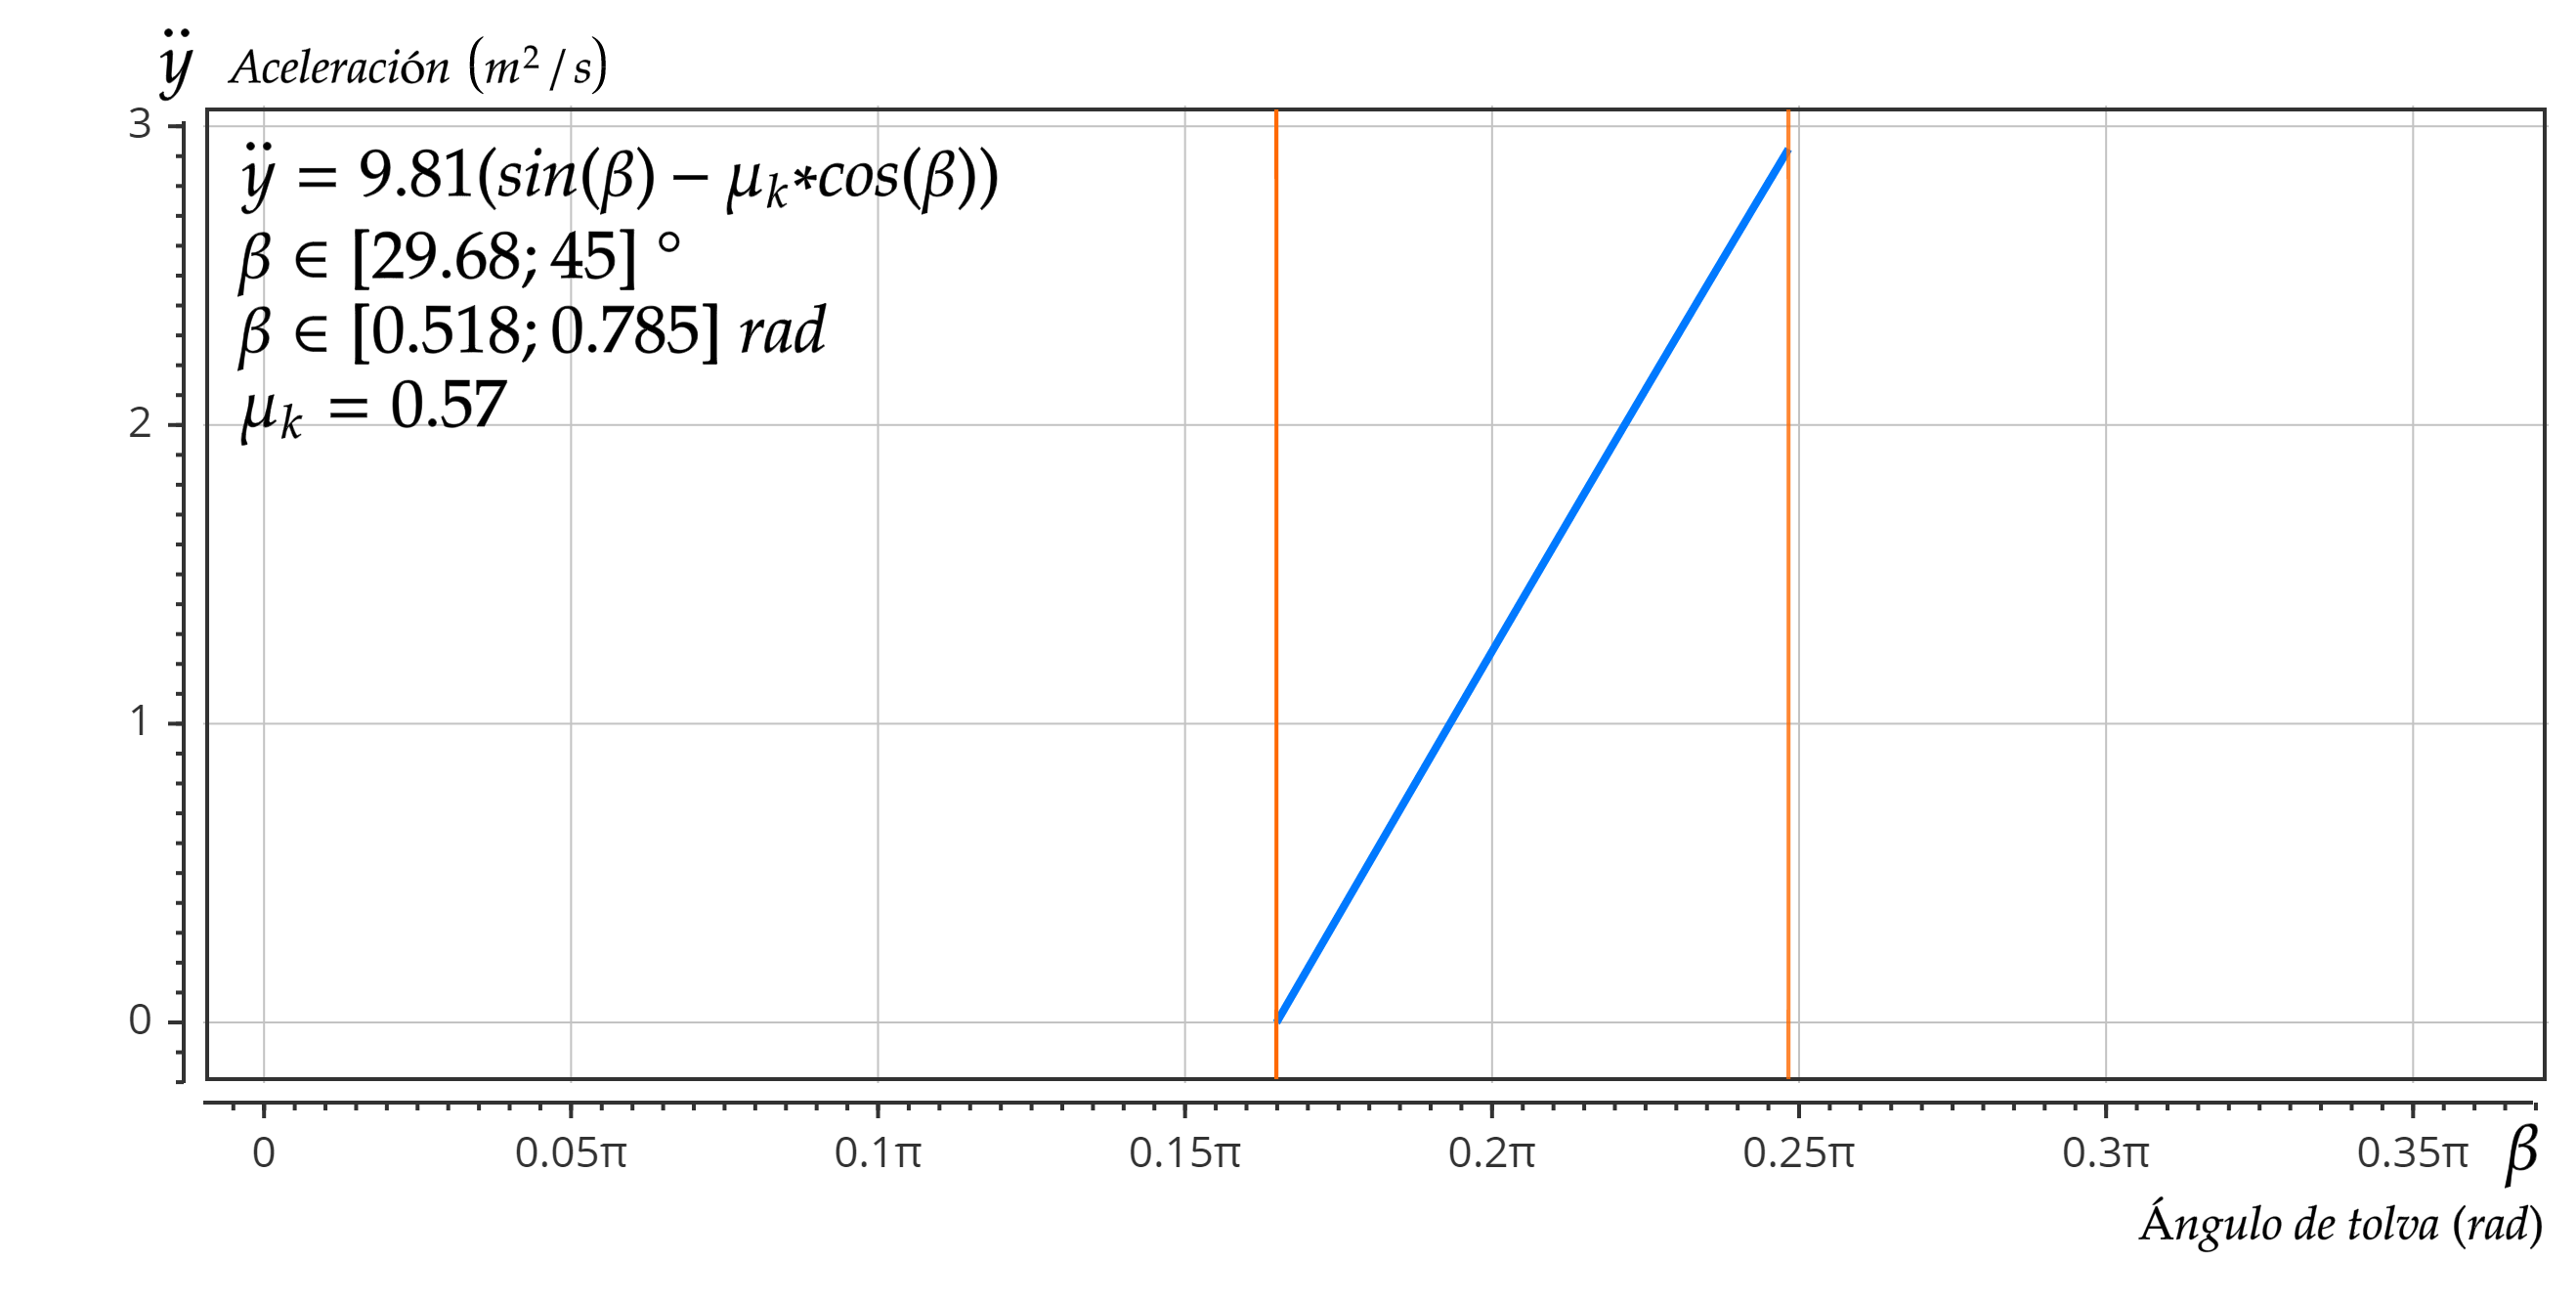
\includegraphics[width=1\textwidth]{chapter5/grafico angulo de tolva vs aceleracion.png}
	\caption{Ángulo de tolva vs aceleración en la trucha}
	\begin{myflushleftportland}
		Fuente: Elaboración propia.
	\end{myflushleftportland}
	\label{fig:grafico angulo de tolva vs aceleracion}
\end{myfigure}

%% NUEVO SUBSECCION X.X.X.X
\subsubsection{Diseño de subsistema de distribución de truchas}

Luego del proceso de procesamiento de imágenes el sistema mediante el algoritmo de clasificación indica al sistema la trayectoria que debe seguir la trucha en tránsito y es accionado por el mecanismo de distribución, mostrado en la Figura \ref{fig:mecanismo de distribucion de truchas}. Dicho mecanismo recibe a la trucha por una única entrada y redirige mediante un juego de compuertas a tres salidas. Finalmente, las truchas son impulsadas al ingresar a tuberías con caudal de agua constante que las transporta hasta las jaulas flotantes correspondientes.

\begin{myfigure}[H]
	\centering
	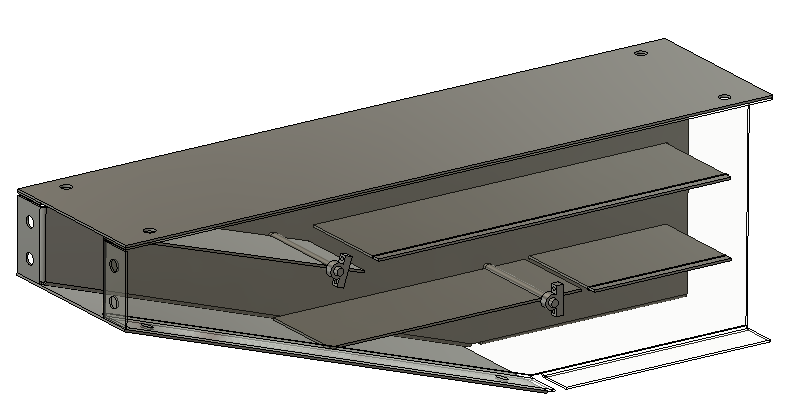
\includegraphics[width=1\textwidth]{chapter5/mecanismo de distribucion de truchas.png}
	\caption{Mecanismo de distribución de truchas}
	\begin{myflushleftportland}
		Fuente: Elaboración propia.
	\end{myflushleftportland}
	\label{fig:mecanismo de distribucion de truchas}
\end{myfigure}

\begin{itemize}
	
	\item \textbf{Selección de mecanismo que acciona la compuerta}
	
	La selección del mecanismo que activa la compuerta tiene requisitos técnicos que son muy importantes, de no funcionar puede parar completamente el proceso general, por lo que se realiza una comparación de los posibles mecanismos a utilizar para hacer girar la compuerta de manera cíclica ordenado por el subsistema de control. La comparación conceptual se muestra en la Tabla \ref{tab:tabla comparativa de conceptos de mecanismos para compuerta} y los conceptos de mecanismos analizados se muestran en la Figura \ref{fig:conceptos de mecanismos de distribucion de truchas}.
	
	\begin{myfigure}[H]
		\centering
		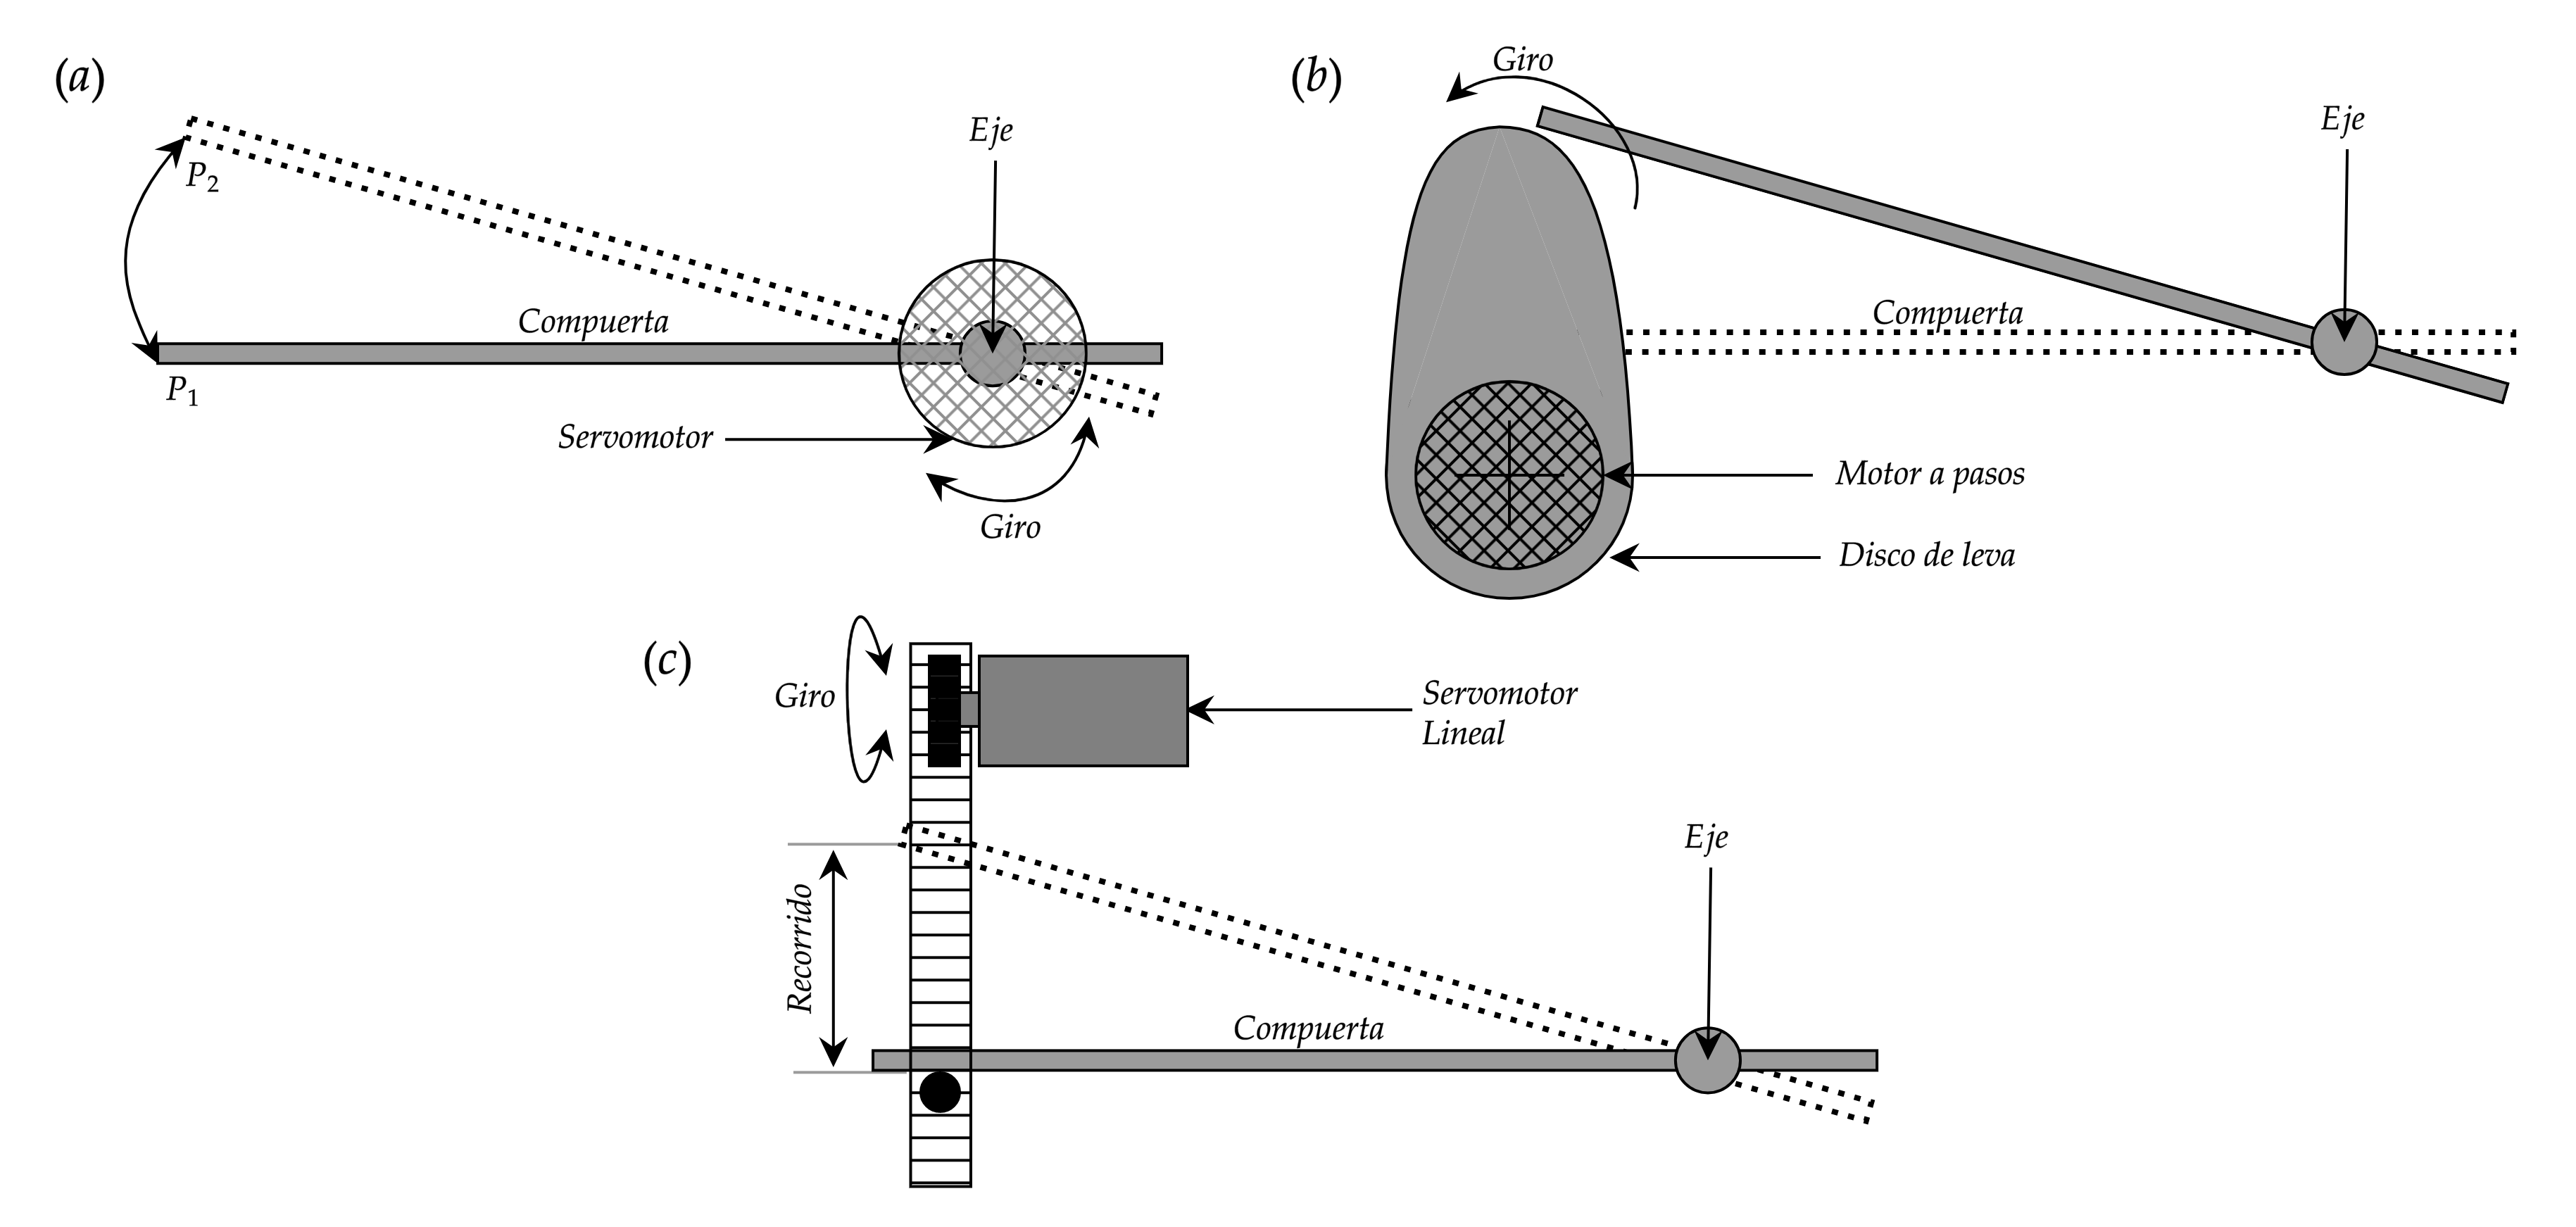
\includegraphics[width=1\textwidth]{chapter5/conceptos de mecanismos de distribucion de truchas.png}
		\caption[Conceptos de mecanismos de distribución de truchas]{(a) Mecanismo de eje servomotor. (b) Mecanismo de tolva y seguidor. (c) Mecanismo de servomotor lineal.}
		\begin{myflushleftportland}
			Fuente: Elaboración propia.
		\end{myflushleftportland}
		\label{fig:conceptos de mecanismos de distribucion de truchas}
	\end{myfigure}
	
	El mecanismo inicialmente propuesto (Figura \ref{fig:conceptos de mecanismos de distribucion de truchas}-a) corresponde a un servomotor conectado al eje de la compuerta del sistema de distribución, los apoyos no son representados en las figuras. El sistema, al efectuar cierta cantidad de giros en un periodo largo\footnote{Una jornada diaria de clasificación puede someter al mecanismo a abrir/cerrar la compuerta en $t_{compuerta}\approx1 s.$ durante $t_{jornadaxdia}=6 h.$} presenta un deterioro considerable en el eje del servomotor, por lo que se analiza un mecanismo de leva-seguidor (Figura \ref{fig:conceptos de mecanismos de distribucion de truchas}-b) que traslada el giro fuera del eje, en un solo sentido y se aplica el giro sobre un extremo de la compuerta, el disco de leva está posicionado para brindar un movimiento armónico al extremo de la compuerta. Así también, se considera un mecanismo de servomotor lineal que mediante una traba en la cremallera desplaza la compuerta hasta la posición requerida mediante giros en los dos sentidos.
	
	\begin{savenotes}	
		\begin{mytable}[H]
			\centering
			\caption{Tabla comparativa de conceptos de mecanismos.}
			\label{tab:tabla comparativa de conceptos de mecanismos para compuerta}
			\begin{tabular}{l|c|c|c|c|}
				\cline{2-5}
				\multicolumn{1}{c|}{\textbf{}} & 
				\textbf{\begin{tabular}[c]{@{}c@{}}Requisitos\\ mínimos\end{tabular}} & \begin{minipage}{\mythirdmaxsizeofcontenttable}\begin{myflushcenter}
						\textbf{Servomotor de rotación posicional}
				\end{myflushcenter}\end{minipage} & 
				\begin{minipage}{\mythirdmaxsizeofcontenttable}\begin{myflushcenter}
						\textbf{Leva y seguidor}
				\end{myflushcenter}\end{minipage} &
				\begin{minipage}{\mythirdmaxsizeofcontenttable}\begin{myflushcenter}
						\textbf{Servomotor lineal}
				\end{myflushcenter}\end{minipage} \\ \hline
				\multicolumn{1}{|l|}{\textbf{Figura}} & - & 
				Figura \ref{fig:conceptos de mecanismos de distribucion de truchas}-a &
				Figura \ref{fig:conceptos de mecanismos de distribucion de truchas}-b &
				Figura \ref{fig:conceptos de mecanismos de distribucion de truchas}-c \\ \hline
				\multicolumn{1}{|l|}{
					\begin{minipage}{\myforthmaxsizeofcontenttable}			
						\textbf{Cantidad de sentidos de giro}
					\end{minipage}
				} & - & 2 & 1 & 2 \\ \hline
				\multicolumn{1}{|l|}{
					\begin{minipage}{\myforthmaxsizeofcontenttable}			
						\textbf{Complejidad mecánica\footnote{Basado en análisis de falla. Calificación cualitativa: baja, media o alta.}}
					\end{minipage}
				} & - & Baja & Alta & Media \\ \hline
				\multicolumn{1}{|l|}{
					\begin{minipage}{\myforthmaxsizeofcontenttable}			
						\textbf{Disponibilidad en el mercado\footnote{Basado en el componente más "difícil" de conseguir.Calificación cualitativa: nacional o internacional}}
					\end{minipage}
				} & - & Nacional & Internacional & Nacional \\ \hline
				\multicolumn{1}{|l|}{
					\begin{minipage}{\myforthmaxsizeofcontenttable}			
						\textbf{Torque máximo\footnote{Basado en situación crítica encontrada derivando la ecuación de torque respectivo. Dónde: $d_{eje}$ es la distancia del centro de gravedad de la compuerta al eje, $d_{leva}$ es la distancia del centro del disco de leva hasta la parte más alejada de este y $d_{ser}$ es diámetro del engranaje en el mecanismo piñón-cremallera del servomotor lineal. ($d_{ser}<d_{leva}<d_{eje}$)} ($\bar{\tau_{max}}$)}
					\end{minipage}
				} & - & $\approx m*g*d_{eje}$ & $\approx m*g*d_{leva}/2$ & $\approx m*g*d_{ser}/4$ \\ \hline
				\multicolumn{1}{|l|}{
					\begin{minipage}{\myforthmaxsizeofcontenttable}			
						\textbf{Desgaste\footnote{Calificación cualitativa: bajo, medio o alto.}}
					\end{minipage}
				} & - & Alto & Bajo & Medio \\ \hline
				\multicolumn{1}{|l|}{
					\begin{minipage}{\myforthmaxsizeofcontenttable}			
						\textbf{Acoplamiento al sistema\footnote{Basado en cantidad de componentes adicionales necesarios para implementar. Calificación cualitativa: bajo, medio o alto.}}
					\end{minipage}
				} & - & Bajo & Medio & Medio \\ \hline
				\multicolumn{1}{|l|}{
					\begin{minipage}{\myforthmaxsizeofcontenttable}			
						\textbf{Ruido generado\footnote{Basado en mecanismo mecánico empleado. Calificación cualitativa: bajo, medio, alto.}}
					\end{minipage}
				} & - & Medio & Bajo & Medio \\ \hline
			\end{tabular}
			\begin{flushleft}	
				Fuente: Elaboración propia.
			\end{flushleft}
		\end{mytable}
	\end{savenotes}	
	
	El mecanismo escogido es el leva y seguidor ya que solo es necesario su giro en un sentido, lo cual disminuye el desgaste, se acopla al sistema sin implementar más soportes que los otros mecanismos, no genera ruido y su fabricación, en caso no se encuentre en el mercado peruano, se puede realizar en un taller nacional.  	
	
	\item \textbf{Diseño de mecanismo que acciona la compuerta}
	
	En la sección anterior se eligió el mecanismo a emplear. El diseño del mecanismo va \textcolor{blue}{[BORRADOR] Agregar descripción. Ut tellus elementum sagittis vitae et leo duis ut diam. Dolor sit amet consectetur adipiscing elit ut aliquam purus sit. [/BORRADOR]}	
	
	
	\begin{myfigure}[H]
		\centering
		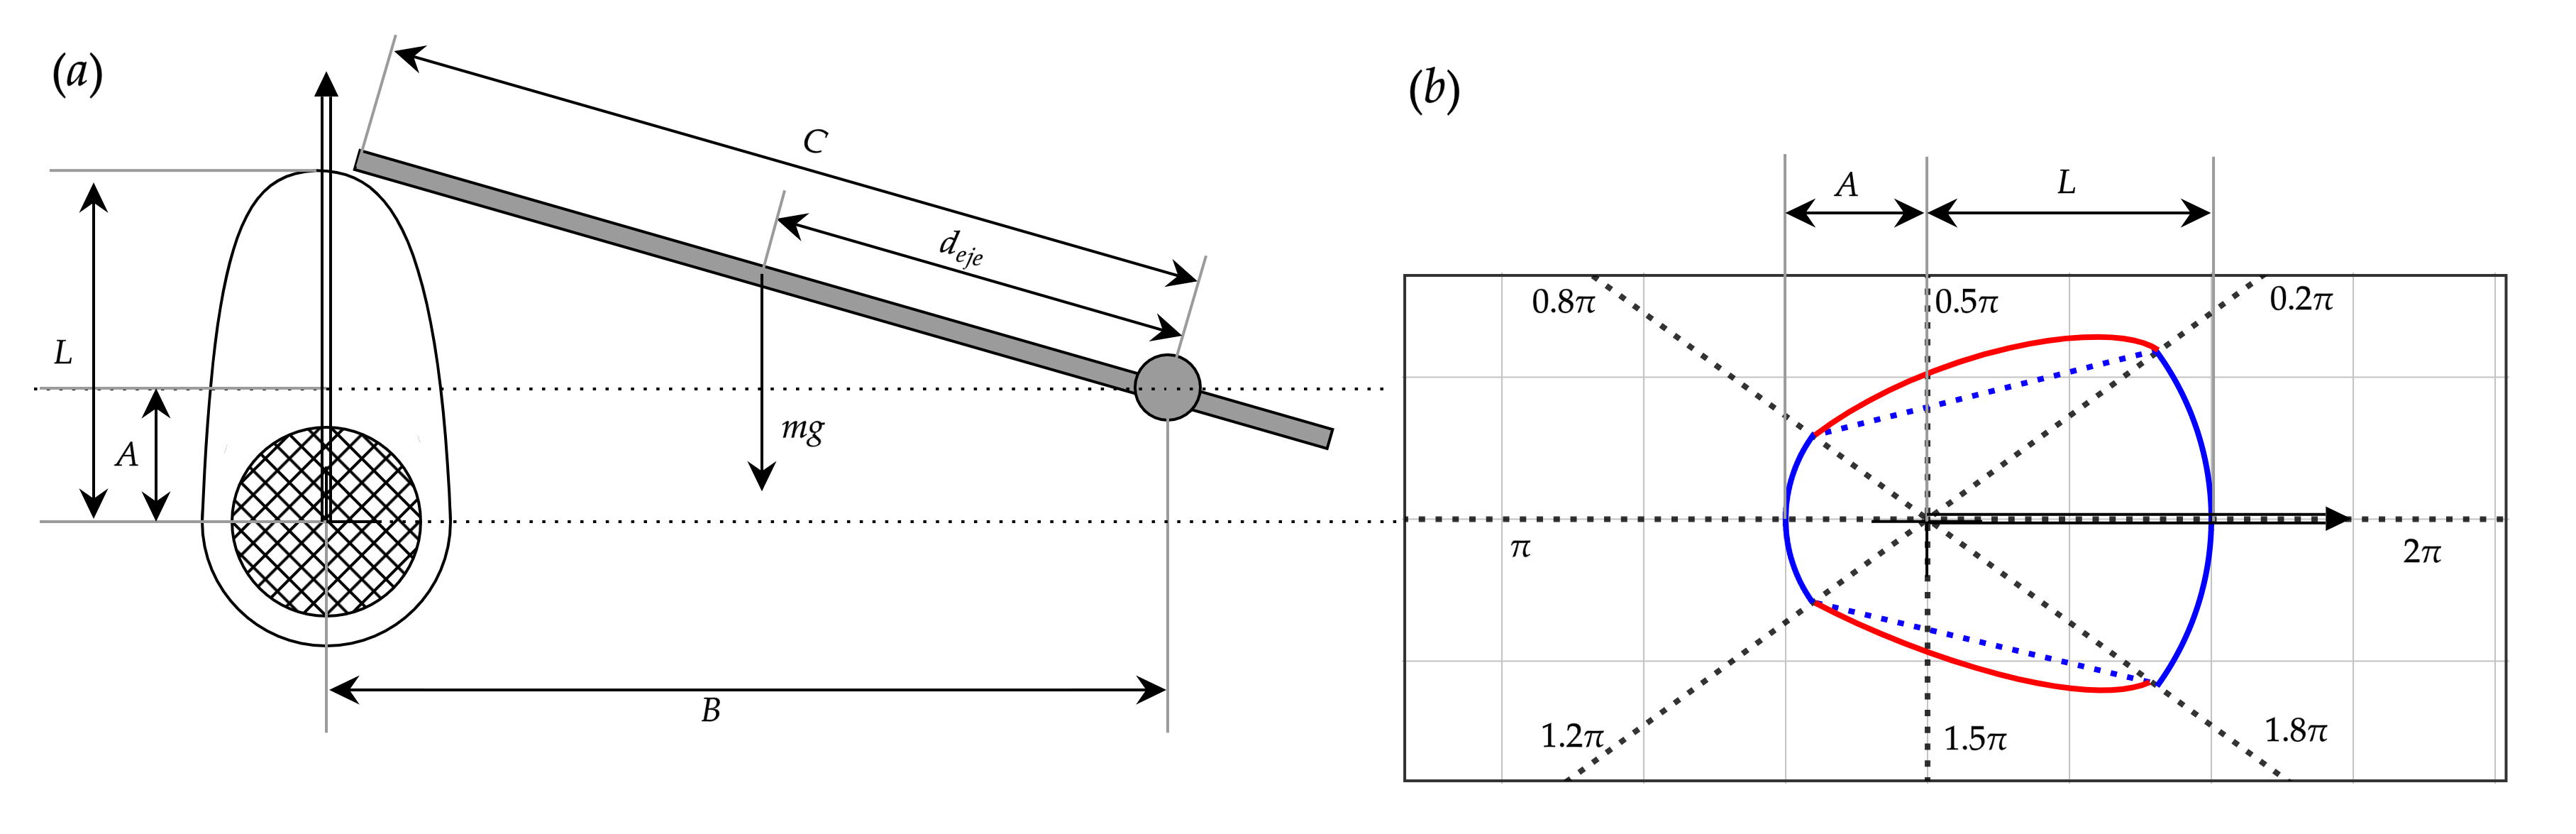
\includegraphics[width=1\textwidth]{chapter5/mecanismo compuerta.png}
		\caption{Mecanismo servomotor-compuerta}
		\begin{myflushleftportland}
			Fuente: Elaboración propia.
		\end{myflushleftportland}
		\label{fig:mecanismo servomotor-compuerta}
	\end{myfigure}
	
	\textcolor{blue}{[BORRADOR] Agregar descripción. Ut tellus elementum sagittis vitae et leo duis ut diam. Dolor sit amet consectetur adipiscing elit ut aliquam purus sit. [/BORRADOR]}	 
	
	\begin{myfigure}[H]
		\centering
		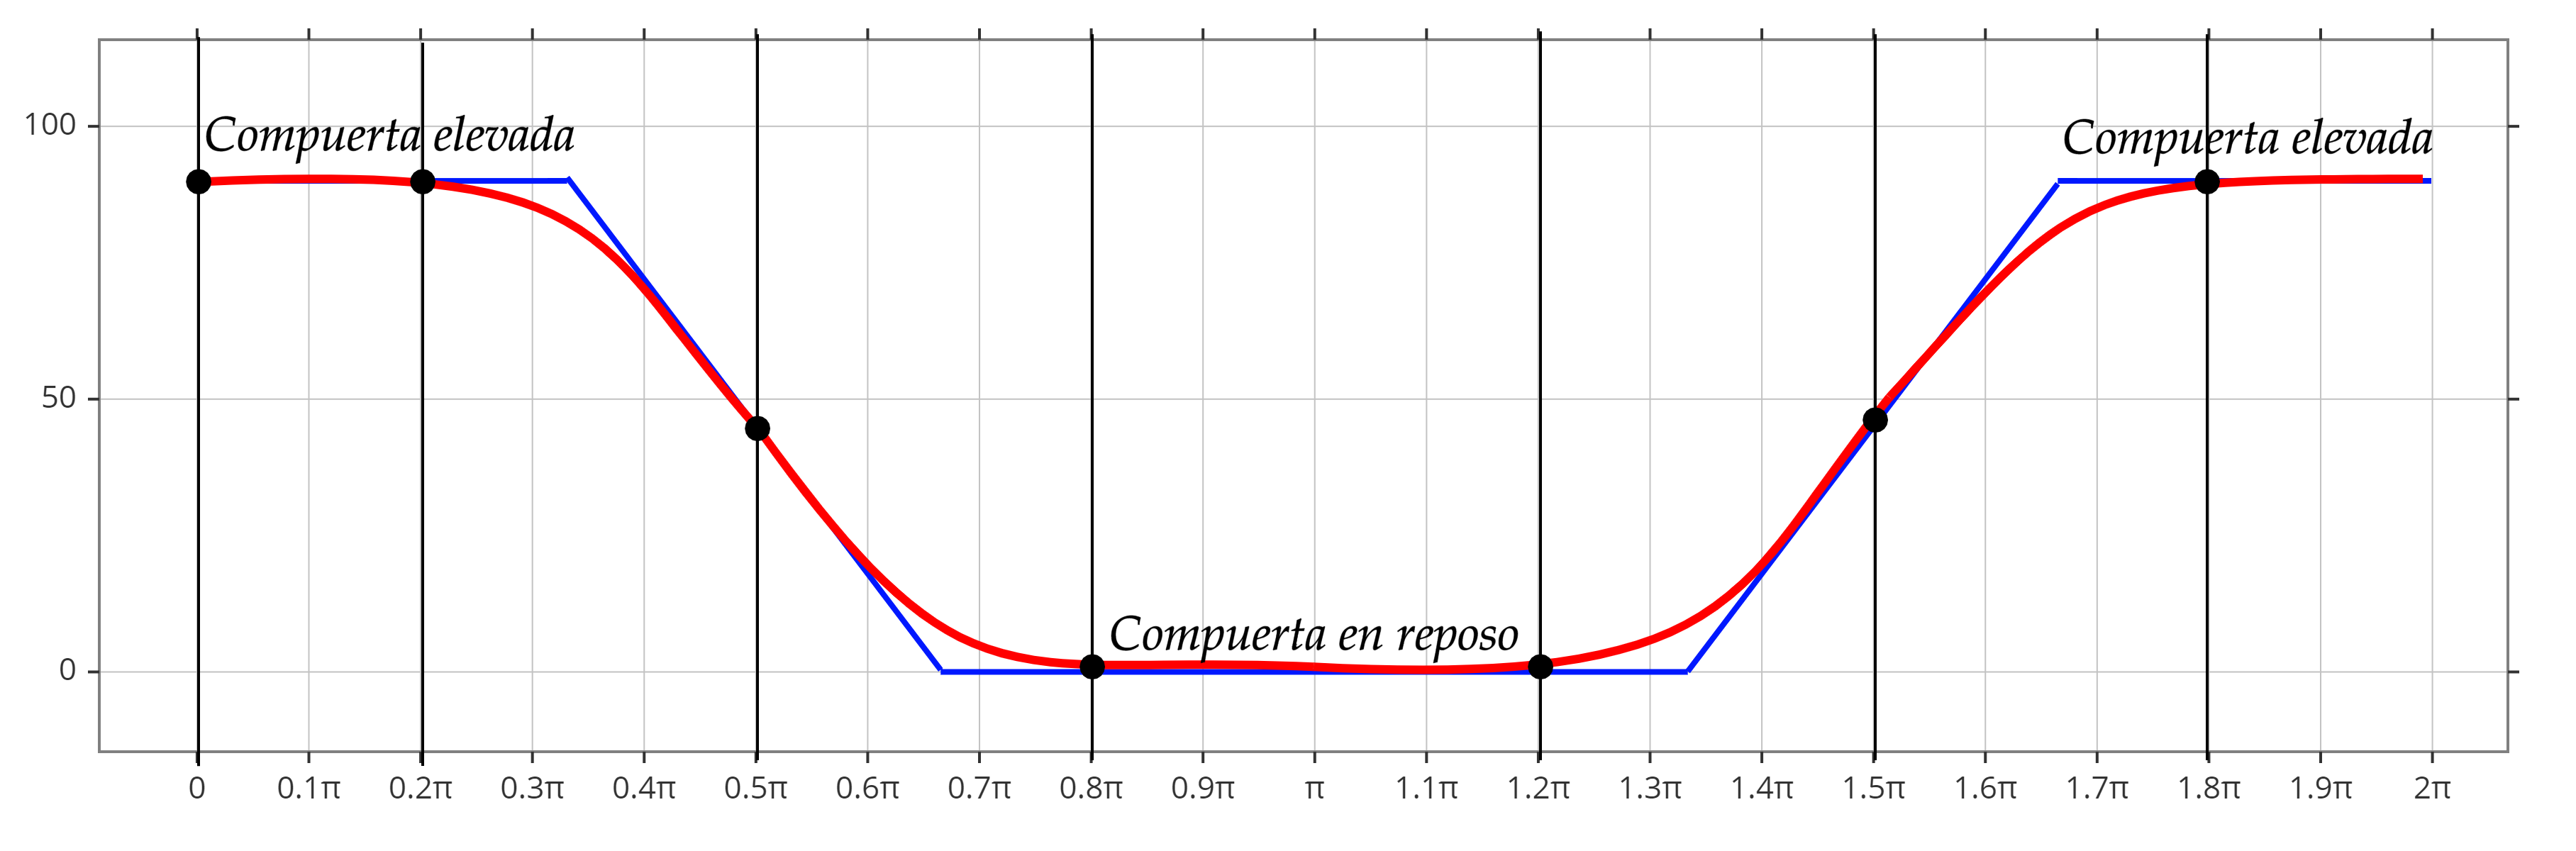
\includegraphics[width=1\textwidth]{chapter5/mecanismo compuerta leva posicionamiento.png}
		\caption{Engranajes del mecanismo de compuertas}
		\begin{myflushleftportland}
			Fuente: Elaboración propia.
		\end{myflushleftportland}
		\label{fig:mecanismo de compuertas engranajes}
	\end{myfigure}
	
	\textcolor{blue}{[BORRADOR] Agregar descripción. Ut tellus elementum sagittis vitae et leo duis ut diam. Dolor sit amet consectetur adipiscing elit ut aliquam purus sit. [/BORRADOR]}	 
	
	\item \textbf{Cálculo de torque y velocidad de giro de compuerta}
	
	
	La fuerza necesaria es simplemente el giro de la compuerta que está unida a un eje y a su vez al mecanismo de engranajes con el servomotor.\textcolor{blue}{[BORRADOR] Explicar selección entre otras cosas .... Además, citar a \cite{ChinchayDeLaCruz2010} en análisis de falla de levas [/BORRADOR]}
	
	\begin{myfigure}[H]
		\centering
		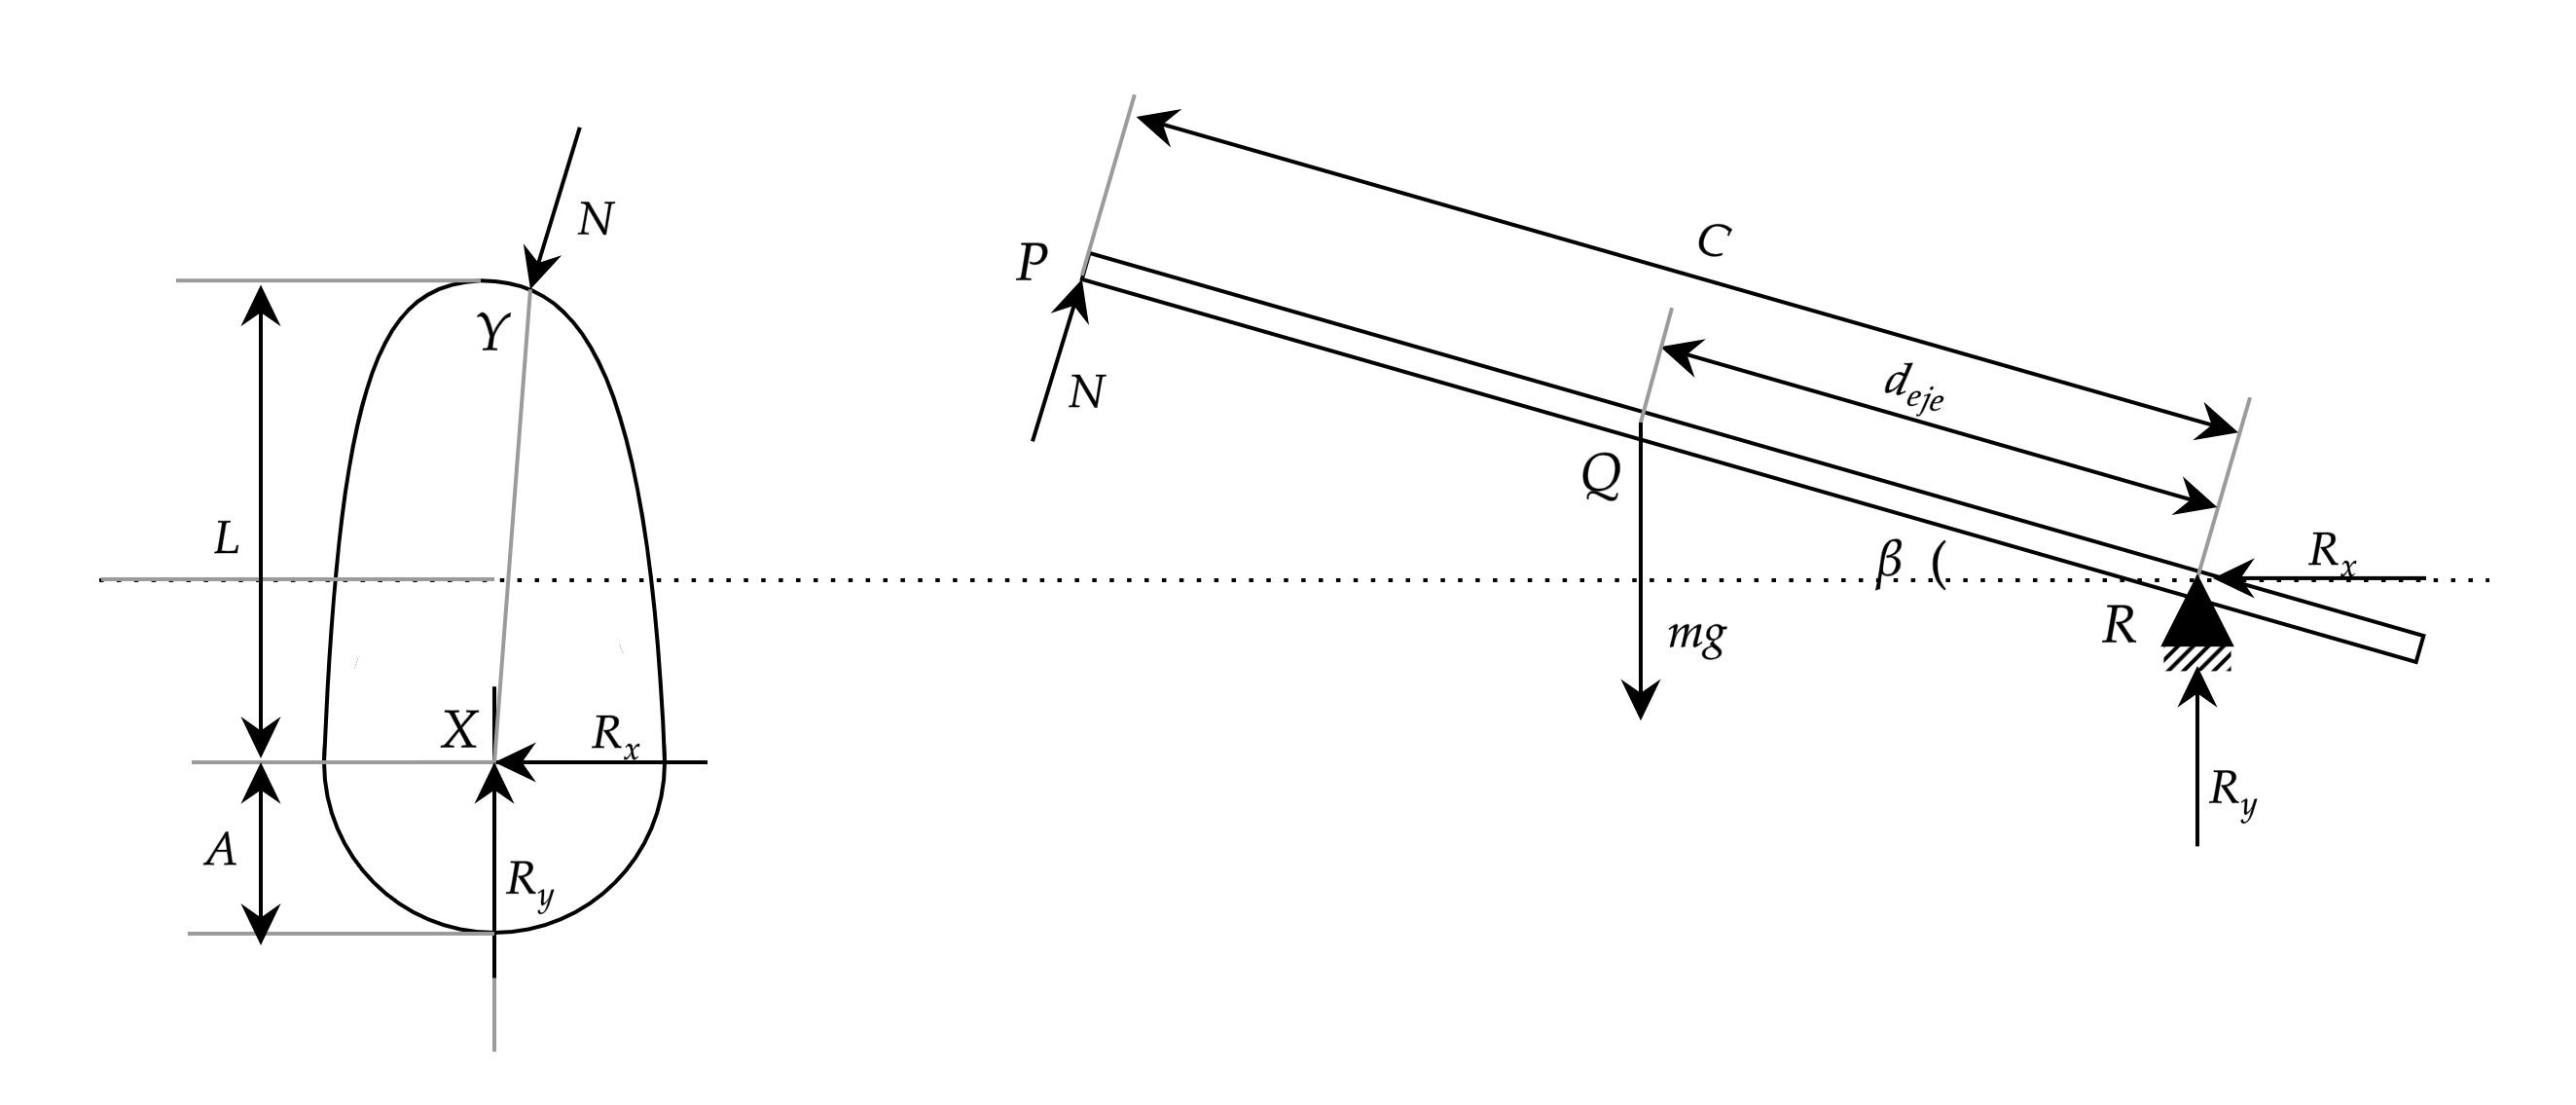
\includegraphics[width=1\textwidth]{chapter5/dlc leva compuerta.png}
		\caption{Diagrama de cuerpo libre del mecanismo de la compuerta.}
		\begin{myflushleftportland}
			Fuente: Elaboración propia.
		\end{myflushleftportland}
		\label{fig:dlc leva compuerta}
	\end{myfigure}
	
	\textcolor{blue}{[BORRADOR] Explicar las Ecuaciones a continuación [/BORRADOR]}
	
	\begin{myequation}\label{eq:calculo fuerza normal}
		\begin{split}
			\sum_{}^{}M_{R}&=m_{compuerta}*g*cos(\beta)*d_{eje}-2*N*d_{eje}=0 \\
			N&=\frac{m*g*cos(\beta)}{2}			
		\end{split}		
	\end{myequation}
	
	\begin{myequation}\label{eq:calculo de torque máximo}
		\begin{split}
			\overrightarrow{T_{X}}&=N*sin(\beta)*L \\
			\overrightarrow{T_{X}}&=\frac{m*g*cos(\beta)}{2}*sin(\beta)*L \\
			\overrightarrow{T_{X}}&=m*g*L*\frac{sin(2\beta)}{2} \\
			\overrightarrow{T_{X_{max}}}&=\frac{m*g*L}{2} \quad (\beta=45^\circ) \\
		\end{split}		
	\end{myequation}
	
	La velocidad de compuertas debe ir acorde a la distancia entre una trucha y la siguiente a esta. \textcolor{blue}{[BORRADOR] Explicar velocidad RPM necesarias y explicar las ecuaciones siguientes [/BORRADOR]}
	
	Ut tellus elementum sagittis vitae et leo duis ut diam. Dolor sit amet consectetur adipiscing elit ut aliquam purus sit. Ut tellus elementum sagittis vitae et leo duis ut diam. Dolor sit amet consectetur adipiscing elit ut aliquam purus sit. 
	
	
	\item \textbf{Selección de motores a paso}
	
	%La selección de los servomotores depende del propósito en la función que se encuentre................
	
	%Este mecanismo mostrado en la Figura acciona la compuerta presentada en la %Figura \ref{fig:compuerta}. El torque necesario del eje es $T_{max}=X (M*mm)$  %y gracias al mecanismo de engranajes puede reducirse a $T_{max_2}=Y (M*mm)$ 
	
	En la Tabla \ref{tab:tabla comparativa de motores a pasos} se muestra una comparación técnica entre tres motores a pasos que cumplen los requisitos mínimos. 
	
	\begin{mytable}[H]
		\centering
		\caption{Tabla comparativa de motores a pasos.}
		\label{tab:tabla comparativa de motores a pasos}
		\begin{tabular}{l|c|c|c|c|}
			\cline{2-5}
			\multicolumn{1}{c|}{\textbf{}}            & \textbf{\begin{tabular}[c]{@{}c@{}}Requisitos\\ mínimos\end{tabular}} & \textbf{1} & \textbf{2} & \textbf{3} \\ \hline
			\multicolumn{1}{|l|}{\textbf{Figura}}     & -                                                                     
			&
			\begin{minipage}{\mythirdmaxsizeofcontenttable}
				\centering
\includegraphics[width=\mythirdmaxsizeimageinsidetable]{chapter5/tablas comparativas/servomotor 1.png} \\ 
				%\begin{myflushcenter}
				%	{\footnotesize Nombre imagen}
				%\end{myflushcenter}
			\end{minipage} 
			&
			\begin{minipage}{\mythirdmaxsizeofcontenttable}
				\centering
\includegraphics[width=\mythirdmaxsizeimageinsidetable]{chapter5/tablas comparativas/servomotor 2.png} \\ 
				%\begin{myflushcenter}
				%	{\footnotesize Nombre imagen}
				%\end{myflushcenter}
			\end{minipage} 
			&
			\begin{minipage}{\mythirdmaxsizeofcontenttable}
				\centering
\includegraphics[width=\mythirdmaxsizeimageinsidetable]{chapter5/tablas comparativas/servomotor 3.png} \\ 
				%\begin{myflushcenter}
				%	{\footnotesize Nombre imagen}
				%\end{myflushcenter}
			\end{minipage} 
			\\ \hline
			\multicolumn{1}{|l|}{\textbf{Fabricante}} & 8                                                                     & 9          & 10         & 11         \\ \hline
			\multicolumn{1}{|l|}{\textbf{A}}          & 12                                                                    & 13         & 14         & 15         \\ \hline
			\multicolumn{1}{|l|}{\textbf{B}}          & 16                                                                    & 17         & 18         & 19         \\ \hline
			\multicolumn{1}{|l|}{\textbf{C}}          & 20                                                                    & 21         & 22         & 23         \\ \hline
			\multicolumn{1}{|l|}{\textbf{D}}          & 24                                                                    & 25         & 26         & 27         \\ \hline
			\multicolumn{1}{|l|}{\textbf{E}}          & 32                                                                    & 33         & 34         & 35         \\ \hline
		\end{tabular}
		\begin{flushleft}	
			Fuente: Imágenes de dominio público y elaboración propia.
		\end{flushleft}
	\end{mytable}
	
	\textcolor{blue}{[BORRADOR] Seleccionar uno y explicar la selección [/BORRADOR]}	
	
	%\item \textbf{Diseño de juego de compuertas programables}
	
	%Descripción.
	
\end{itemize}

%%%%%%%%%%%%%%%%%%%%%%%%%%%%%%%%%%%%%%%%%%%%%%
%% NUEVO SUBSECCION X.X.X.X
%\subsubsection{Selección de reja accionada por motor}

%Esta compuerta puede ser reemplazada por una tapa para la tolva de recepción de truchas. En el presente trabajo se decide optar por eliminar este componente.

%\textcolor{blue}{[BORRADOR] ¿Se puede eliminar este inciso en caso no lo use? [/BORRADOR]} 
%%%%%%%%%%%%%%%%%%%%%%%%%%%%%%%%%%%%%%%%%%%%%%

%% NUEVO SUBSECCION X.X.X.X
\subsubsection{Diseño de subsistema de tuberías}

Las tuberías del sistema tienen como propósito abastecer de un flujo de agua constante a la máquina mientras está en funcionamiento. Cuatro canales de tuberías se abastecen de un flujo mediante este subsistema, accionado por bombas de agua y controlados por electroválvulas y sensores de caudal. Esto permite un correcto abastecimiento que no perjudique a las truchas. En las siguientes subsecciones se detalla el dimensionamiento de las tuberías, cálculo de caudales apropiados, selección de electroválvulas, su control asociado y selección de bombas de agua.

\begin{itemize}
	
	\item \textbf{Diseño de tuberías}
	
	\textcolor{blue}{[BORRADOR] Explicar características y requerimientos técnicos que se necesitarán en las tuberías [/BORRADOR]} 
	
	\begin{myfigure}[H]
		\centering
		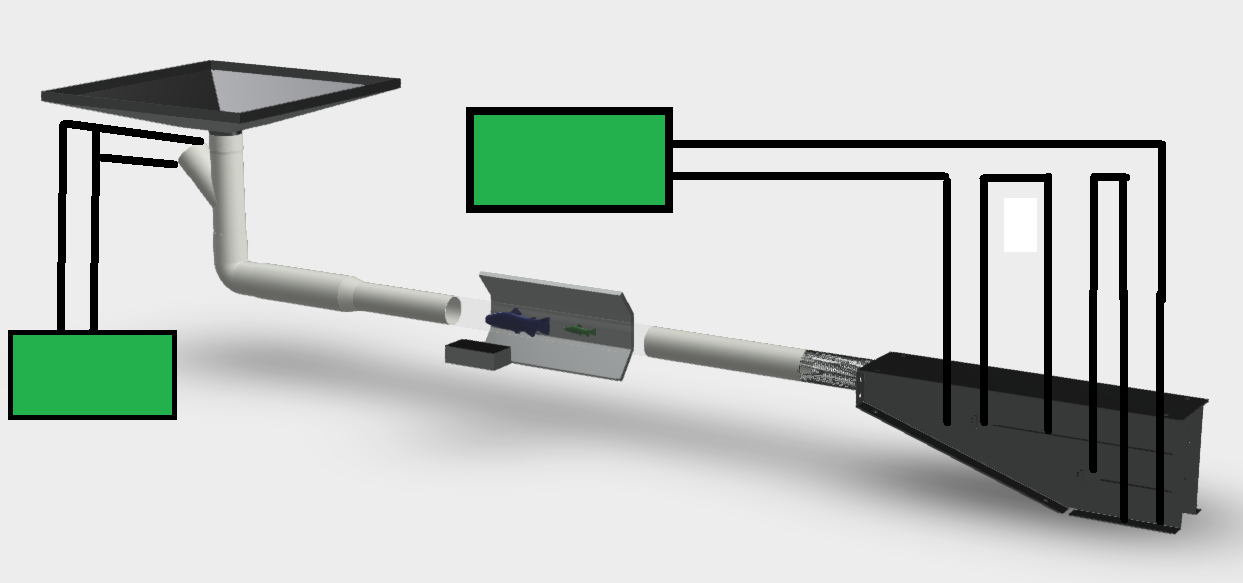
\includegraphics[width=1\textwidth]{chapter5/concepto optimo tuberias.png}
		\caption{Diseño de tuberías para el concepto óptimo}
		\begin{myflushleftportland}
			Fuente: Elaboración propia.
		\end{myflushleftportland}
		\label{fig:concepto optimo tuberias}
	\end{myfigure}
	
	\item \textbf{Diseño de filtro único incluido}
	
	\textcolor{blue}{[BORRADOR] Explicar características y requerimientos técnicos que se necesita para que pase una trucha por vez [/BORRADOR]} 
	
	\begin{myfigure}[H]
		\centering
		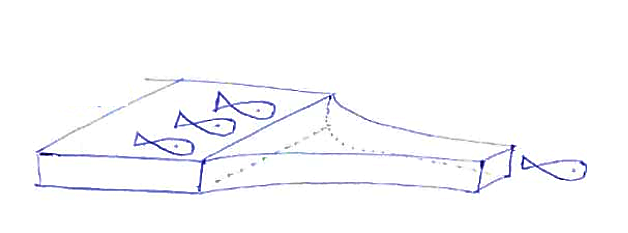
\includegraphics[width=0.25\textwidth]{chapter5/filtro unico.png}
		\caption{Filtro único}
		\begin{myflushleftportland}
			Fuente: Elaboración propia.
		\end{myflushleftportland}
		\label{fig:filtro unico}
	\end{myfigure}
	
	\item \textbf{Selección de caudales apropiados} 
	
	En la Sección \ref{sssec:seleccion de microprocesador} se calcula la velocidad máxima, aproximada, de nado de las truchas arcoíris: $16 (cm/s)$. La Ecuación \ref{eq:calculo de caudal maximo} toma el valor de \textit{$v_{max}=16 (cm/s)$}  y el \textcolor{blue}{[BORRADOR] Terminar de redactar [/BORRADOR]} 
	
	\begin{myequation}\label{eq:calculo de caudal maximo}
		\begin{split}
			Q_{max} & = v_{max}*A \\
			Q_{max} & = 16*\frac{\pi}{4}*(r_{int})^2 \\
			Q_{max} & = 16*\frac{\pi}{4}*(9.1)^2 \\
			Q_{max} & = 1040.62 
		\end{split}		
	\end{myequation}

	Donde: $Q_{max} (cm^3/s)$ es el caudal máximo, $v_{max} (cm/s)$ es la velocidad máxima del agua, $r_{int} (cm)$.
	
	\textcolor{blue}{[BORRADOR] Explicar los caudales apropiados para cada salida, son 4 salidas para dos bombas de agua distintas [/BORRADOR]} 	
	
	\item \textbf{Selección de las electroválvulas}
	
	Los valores límites que se tendrían que controlar mediante las electroválvulas pertenecen al rango $[0;12345] (m^3/s)$. En la Tabla \ref{tab:tabla comparativa de electrovalvulas} se muestran algunso modelos comerciales que cumplen con estos requerimientos. \textcolor{blue}{[BORRADOR] Terminar de calcular caudal adecuado, luego se podra seleccionar electroválvula [/BORRADOR]}
	
	\begin{mytable}[H]
		\centering
		\caption{Tabla comparativa de electroválvulas}
		\label{tab:tabla comparativa de electrovalvulas}
		\begin{tabular}{l|c|c|c|c|}
			\cline{2-5}
			\multicolumn{1}{c|}{\textbf{}}            & \textbf{\begin{tabular}[c]{@{}c@{}}Requisitos\\ mínimos\end{tabular}} & \textbf{1} & \textbf{2} & \textbf{3} \\ \hline
			\multicolumn{1}{|l|}{\textbf{Figura}}   & -   
			&
			\begin{minipage}{\mythirdmaxsizeofcontenttable}
				\centering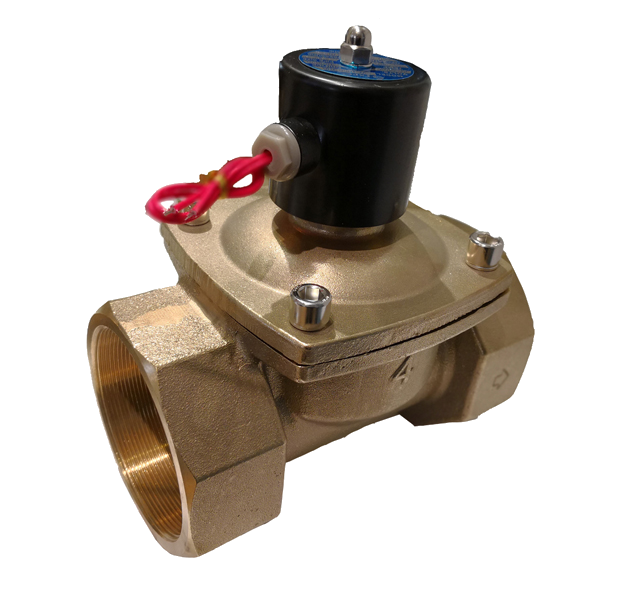
\includegraphics[width=\mythirdmaxsizeimageinsidetable]{chapter5/tablas comparativas/electrovalvula 1.png} \\ 
				%\begin{myflushcenter}
				%	{\footnotesize Nombre imagen}
				%\end{myflushcenter}
			\end{minipage} 
			&
			\begin{minipage}{\mythirdmaxsizeofcontenttable}
				\centering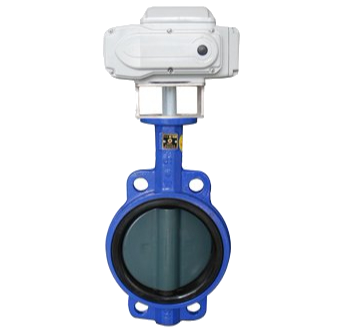
\includegraphics[width=\mythirdmaxsizeimageinsidetable]{chapter5/tablas comparativas/electrovalvula 2.png} \\ 
				%\begin{myflushcenter}
				%	{\footnotesize Nombre imagen}
				%\end{myflushcenter}
			\end{minipage} 
			&
			\begin{minipage}{\mythirdmaxsizeofcontenttable}
				\centering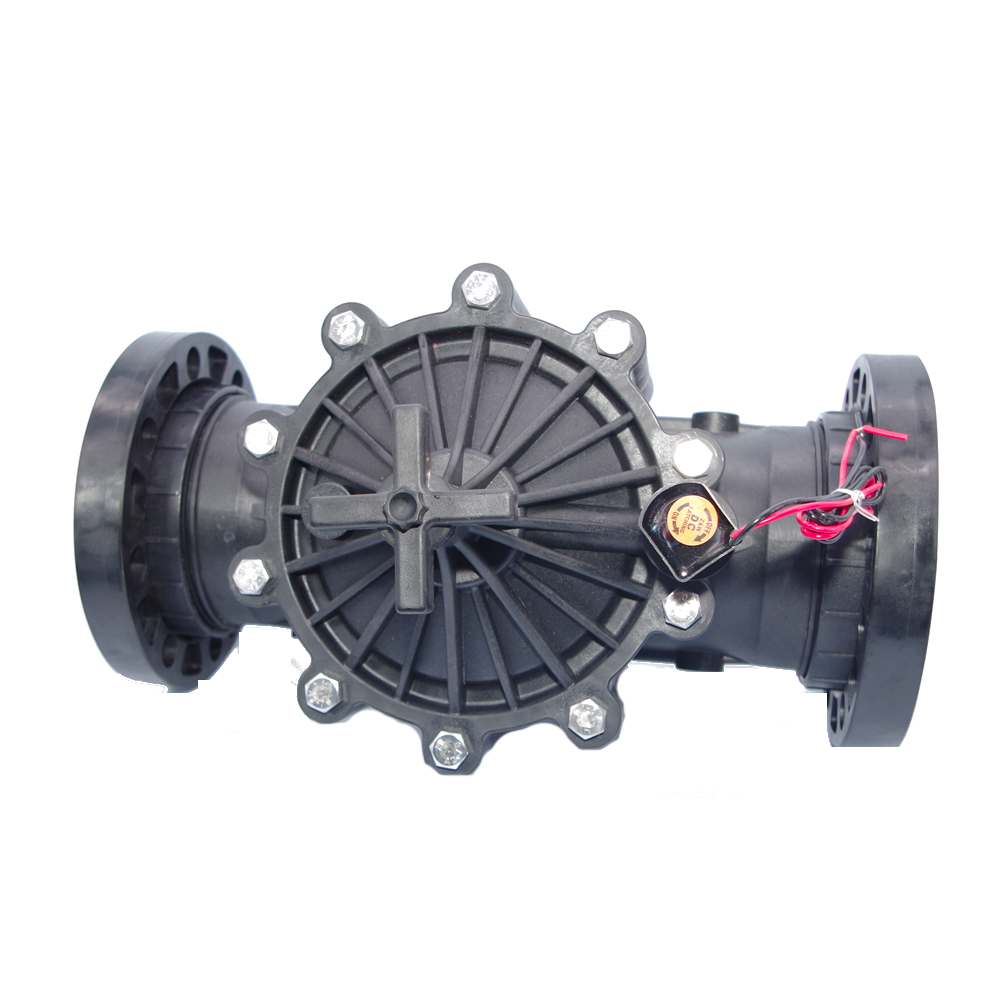
\includegraphics[width=\mythirdmaxsizeimageinsidetable]{chapter5/tablas comparativas/electrovalvula 3.png} \\ 
				%\begin{myflushcenter}
				%	{\footnotesize Nombre imagen}
				%\end{myflushcenter}
			\end{minipage}	\\ \hline
			\multicolumn{1}{|l|}{\textbf{Fabricante}} & 8                                                                     & 9          & 10         & 11         \\ \hline
			\multicolumn{1}{|l|}{\textbf{A}}          & 12                                                                    & 13         & 14         & 15         \\ \hline
			\multicolumn{1}{|l|}{\textbf{B}}          & 16                                                                    & 17         & 18         & 19         \\ \hline
			\multicolumn{1}{|l|}{\textbf{C}}          & 20                                                                    & 21         & 22         & 23         \\ \hline
			\multicolumn{1}{|l|}{\textbf{D}}          & 24                                                                    & 25         & 26         & 27         \\ \hline
			\multicolumn{1}{|l|}{\textbf{E}}          & 32                                                                    & 33         & 34         & 35         \\ \hline
		\end{tabular}	
		\begin{flushleft}			
			Fuente: Imágenes de dominio público y elaboración propia. 
		\end{flushleft}
	\end{mytable}
	
	\textcolor{blue}{[BORRADOR] Escoger una electroválvula y argumentar la decisión [/BORRADOR]}
	
	\item \textbf{Control de los caudales de agua}
	
	Los caudales que generan las bombas de agua sirven para impulsar a las truchas por el interior de la máquina. \textcolor{blue}{[BORRADOR] Dar más detalle en este punto [/BORRADOR]}
	
	\textcolor{blue}{[BORRADOR] Explicar el diagrama de actuadores, sensores,... [/BORRADOR]}
	
	\begin{myfigure}[H]
		\centering
		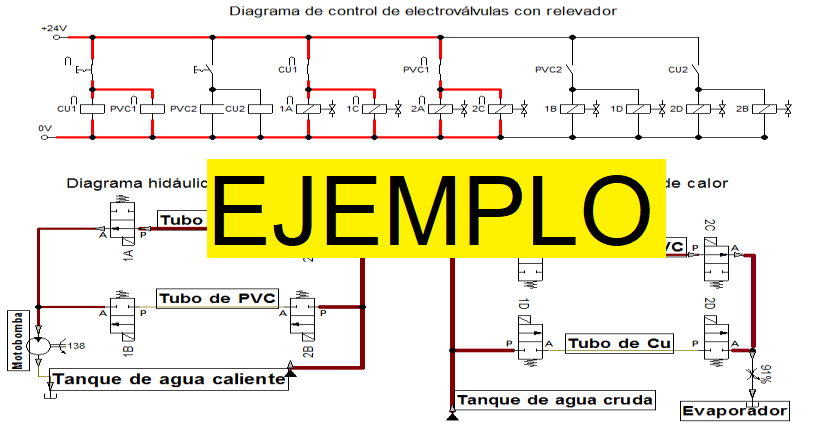
\includegraphics[width=1\textwidth]{chapter5/diagrama de control de electrovalvulas.png}
		\caption{Diagrama de control de electrovalvulas}
		\begin{myflushleftportland}
			Fuente: Elaboración propia.
		\end{myflushleftportland}
		\label{fig:diagrama de control de electrovalvulas}
	\end{myfigure}
	
	\textcolor{blue}{[BORRADOR] Explicar el control escogido, quizás PID para las electroválvulas [/BORRADOR]}
	
	\begin{myfigure}[H]
		\centering
		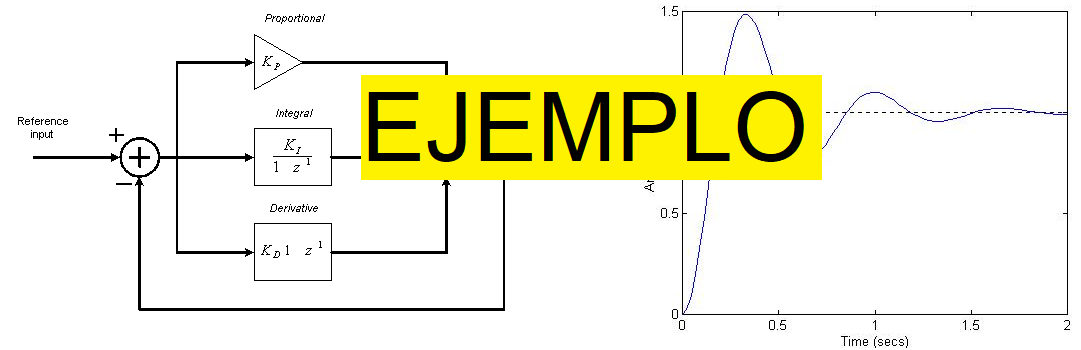
\includegraphics[width=1\textwidth]{chapter5/control electrovalvulas pid.png}
		\caption{Control PID de una electrovalvula}
		\begin{myflushleftportland}
			Fuente: Elaboración propia.
		\end{myflushleftportland}
		\label{fig:control electrovalvulas pid}
	\end{myfigure}
	
	\textcolor{blue}{[BORRADOR] Calcular los valores PID [/BORRADOR]}
	
	\textcolor{blue}{[BORRADOR] Explicar qué dispositivo llevará el control PID: MCU, board especial, etc?? [/BORRADOR]}	
	
\end{itemize}

%% NUEVO SUBSECCION X.X.X.X
\subsubsection{Selección de bomba de agua sumergible}


En la subsección anterior \textit{"Diseño de subsistema de tuberías"} se calcularon los caudales apropiados para el sistema. La bomba de agua sumergible se selecciona de acuerdo a características técnicas como potencia, consumo de energía, horas de uso continuo, entre otras que se exponen en la Tabla \ref{tab:tabla comparativa de bombas de agua sumergibles}.


\begin{mytable}[H]
	\centering
	\caption{Tabla comparativa de bombas de agua sumergibles.}
	\label{tab:tabla comparativa de bombas de agua sumergibles}
	\begin{tabular}{l|c|c|c|c|}
		\cline{2-5}
		\multicolumn{1}{c|}{\textbf{}}            & \textbf{\begin{tabular}[c]{@{}c@{}}Requisitos\\ mínimos\end{tabular}} & \textbf{1} & \textbf{2} & \textbf{3} \\ \hline
		\multicolumn{1}{|l|}{\textbf{Figura}}     & -                                                                     
		&
		\begin{minipage}{\mythirdmaxsizeofcontenttable}
			\centering
\includegraphics[width=\mythirdmaxsizeimageinsidetable]{chapter5/tablas comparativas/bomba de agua sumergible 1.png} \\ 
			%\begin{myflushcenter}
			%	{\footnotesize Nombre imagen}
			%\end{myflushcenter}
		\end{minipage} 
		&
		\begin{minipage}{\mythirdmaxsizeofcontenttable}
			\centering
\includegraphics[width=\mythirdmaxsizeimageinsidetable]{chapter5/tablas comparativas/bomba de agua sumergible 2.png} \\ 
			%\begin{myflushcenter}
			%	{\footnotesize Nombre imagen}
			%\end{myflushcenter}
		\end{minipage} 
		&
		\begin{minipage}{\mythirdmaxsizeofcontenttable}
			\centering
\includegraphics[width=\mythirdmaxsizeimageinsidetable]{chapter5/tablas comparativas/bomba de agua sumergible 3.png} \\ 
			%\begin{myflushcenter}
			%	{\footnotesize Nombre imagen}
			%\end{myflushcenter}
		\end{minipage} 
		\\ \hline
		\multicolumn{1}{|l|}{\textbf{Fabricante}} & 8                                                                     & 9          & 10         & 11         \\ \hline
		\multicolumn{1}{|l|}{\textbf{A}}          & 12                                                                    & 13         & 14         & 15         \\ \hline
		\multicolumn{1}{|l|}{\textbf{B}}          & 16                                                                    & 17         & 18         & 19         \\ \hline
		\multicolumn{1}{|l|}{\textbf{C}}          & 20                                                                    & 21         & 22         & 23         \\ \hline
		\multicolumn{1}{|l|}{\textbf{D}}          & 24                                                                    & 25         & 26         & 27         \\ \hline
		\multicolumn{1}{|l|}{\textbf{E}}          & 32                                                                    & 33         & 34         & 35         \\ \hline
	\end{tabular}
	\begin{flushleft}	
		Fuente: Imágenes de dominio público y elaboración propia.
	\end{flushleft}
\end{mytable}

\textcolor{blue}{[BORRADOR] Explicar la elección [/BORRADOR]}


%% NUEVA SECCIÓN X.X.X
\subsection{Subsistema de procesamiento de imágenes}
\label{ssec:subsistema de procesamiento de imágenes}

Este subsistema consiste obtener una serie de imágenes de una trucha en tránsito e indicar al sistema a dónde debería dirigirse una trucha determinada. El subsistema debe clasificar y contar truchas, con dicha finalidad necesita de la selección de una cámara y generar el ambiente adecuado para obtener las imágenes. Explicado los objetivos del subsistema, en las siguientes líneas se detalla: la selección del sensor infrarrojo, la selección de cámara estéreo, la selección de iluminación adecuada y la selección de algoritmos.

%% NUEVO SUBSECCION X.X.X.X
\subsubsection{Selección del sensor infrarrojo}

El sensor infrarrojo tiene como objetivo activar el algoritmo de detección y conteo de truchas por un determinado periodo de tiempo con la finalidad de evitar un sobre uso de los recursos computacionales. El sensor infrarrojo está unos centímetros antes de la parte que la cámara captura y su posición es como se muestra en las Figura \ref{fig:posicion sensor infrarrojo}.

\begin{myfigure}[H]
	\centering
	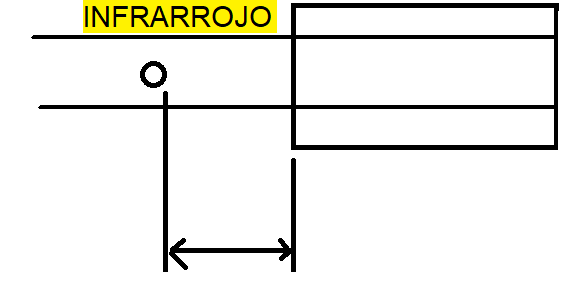
\includegraphics[width=1\textwidth]{chapter5/posicion sensor infrarrojo.png}
	\caption{Posicionamiento del sensor infrarrojo}
	\begin{myflushleftportland}
		Fuente: Elaboración propia.
	\end{myflushleftportland}
	\label{fig:posicion sensor infrarrojo}
\end{myfigure}

Ya que los haces de luz cambian de dirección debido a la refracción\footnote{\cite{Hecht2017}.}, cuando varía de un medio a otro, se calcula esta desviación para la adecuada detección de objetos que pasen por la tubería. La representación gráfica de la situación se expone en la Figura \ref{fig:analisis de posicion de luz infrarroja}.

\begin{myfigure}[H]
	\centering
	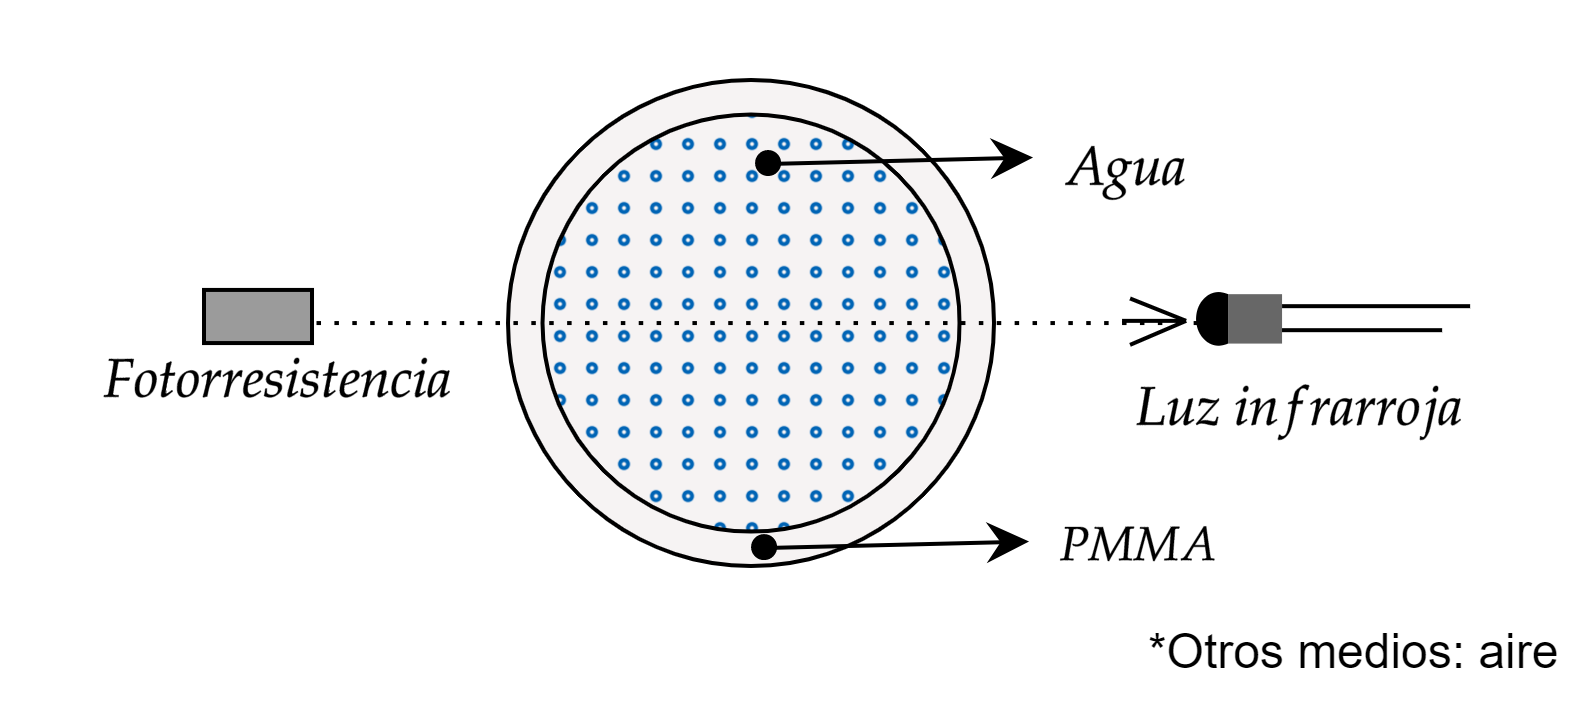
\includegraphics[width=0.75\textwidth]{chapter5/analisis de posicion de luz infrarroja.png}
	\caption{Análisis de posición de luz infrarroja}
	\begin{myflushleftportland}
		Fuente: Elaboración propia.
	\end{myflushleftportland}
	\label{fig:analisis de posicion de luz infrarroja}
\end{myfigure}

El problema se muestra en la Figura \ref{fig:calculo de posicion de luz infrarroja}. Cabe mencionar que se conocen los siguientes valores $n_{PMMA}=1.5$\footnote{Propiedades ópticas mostradas en la Tabla \ref{tab:tabla comparativa de propiedades entre pmma vs pvdf vs petg}. \cite{Berins1991}}, $n_{aire}\approx1$, $n_{agua}=1.33$\footnote{Índices de refracción: \cite{Hecht2017}.}, $d_{1}=d_{2}=10 mm.$, $e=3 mm.$ y $d_{int}=85 mm.$ ,y se asume, para simplificar el problema, la emisión de la luz como proveniente de un punto único ($S$).

\begin{myfigure}[H]
	\centering
	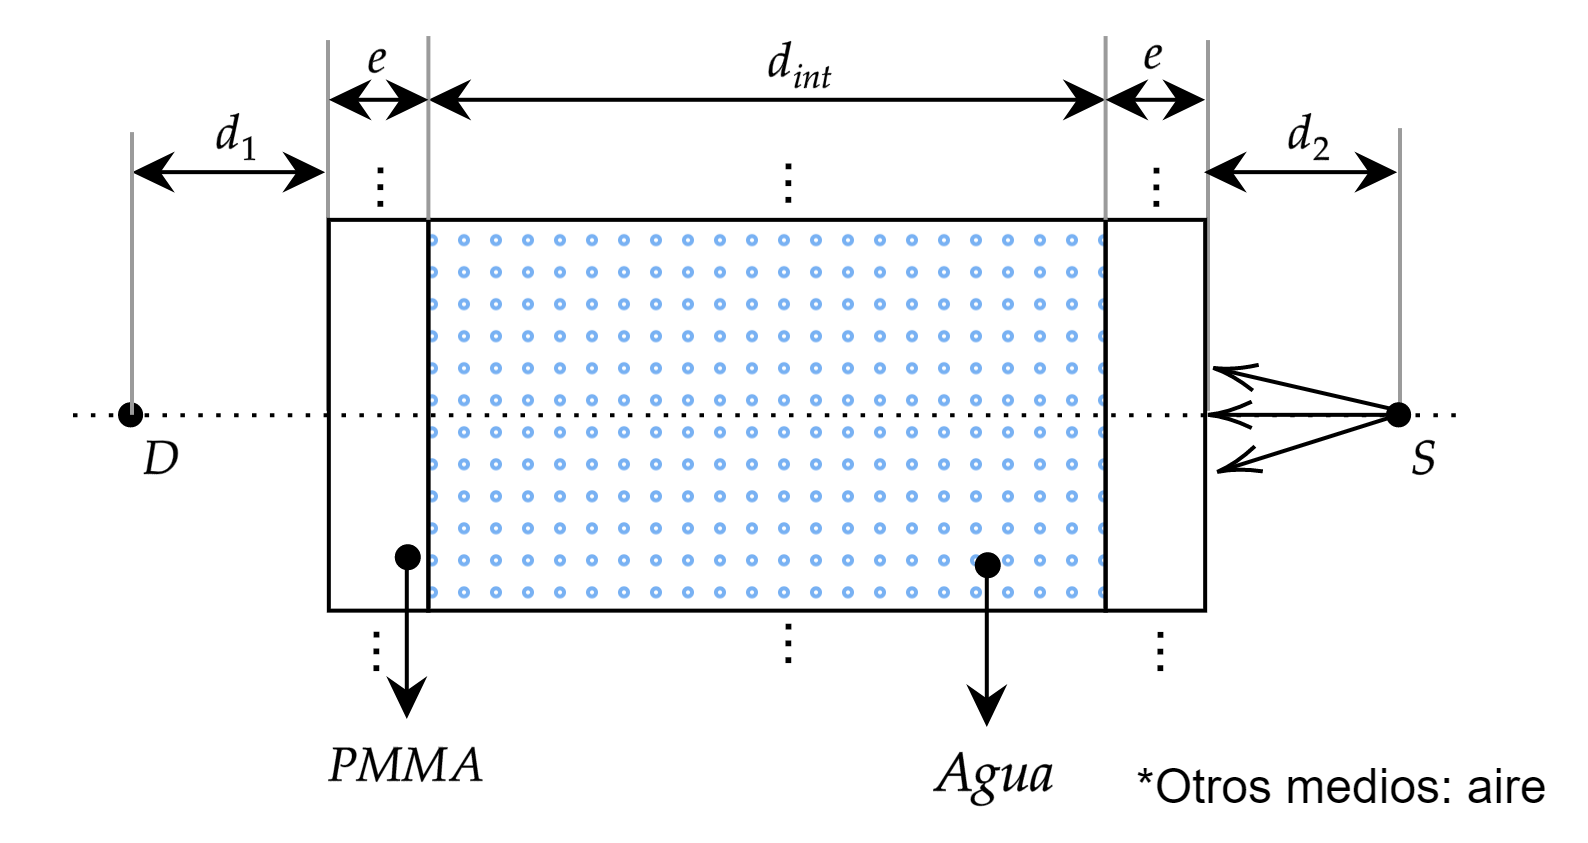
\includegraphics[width=0.75\textwidth]{chapter5/calculo de posicion de luz infrarroja.png}
	\caption{Cálculo de posición de luz infrarroja}
	\begin{myflushleftportland}
		Fuente: Elaboración propia.
	\end{myflushleftportland}
	\label{fig:calculo de posicion de luz infrarroja}
\end{myfigure}

Para el cálculo de desviación de los haces de luz se emplea la ley de refracción, matemáticamente mostrada en la Ecuación \ref{eq:ecuacion de snell}. Donde: $\theta_{i}$ es el ángulo de incidencia respecto a la normal del primer medio, $\theta_{t}$ es el ángulo de refracción respecto a la normal.

\begin{myequation}\label{eq:ecuacion de snell}
	\begin{split}
		n_{i}*sin(\theta_{i})&=n_{t}*sin(\theta_{t})
	\end{split}		
\end{myequation}

En la Figura \ref{fig:calculo distancia maxima de desviacion de haz de luz en condiciones ideales} se analiza el caso crítico cuando $\theta_{1}\approx5^\circ$. Con la Ecuación \ref{eq:ecuacion de snell} se puede calcular las distancias de desviación por refracción. Por ejemplo, En la Ecuación \ref{eq:calculo distancia maxima de desviacion de haz de luz en condiciones ideales} el valor de $h_{x}$ es la distancia proyectada: $h_{x}=d_{x}*tan(\theta_{x})$.

\begin{myfigure}[H]
	\centering
	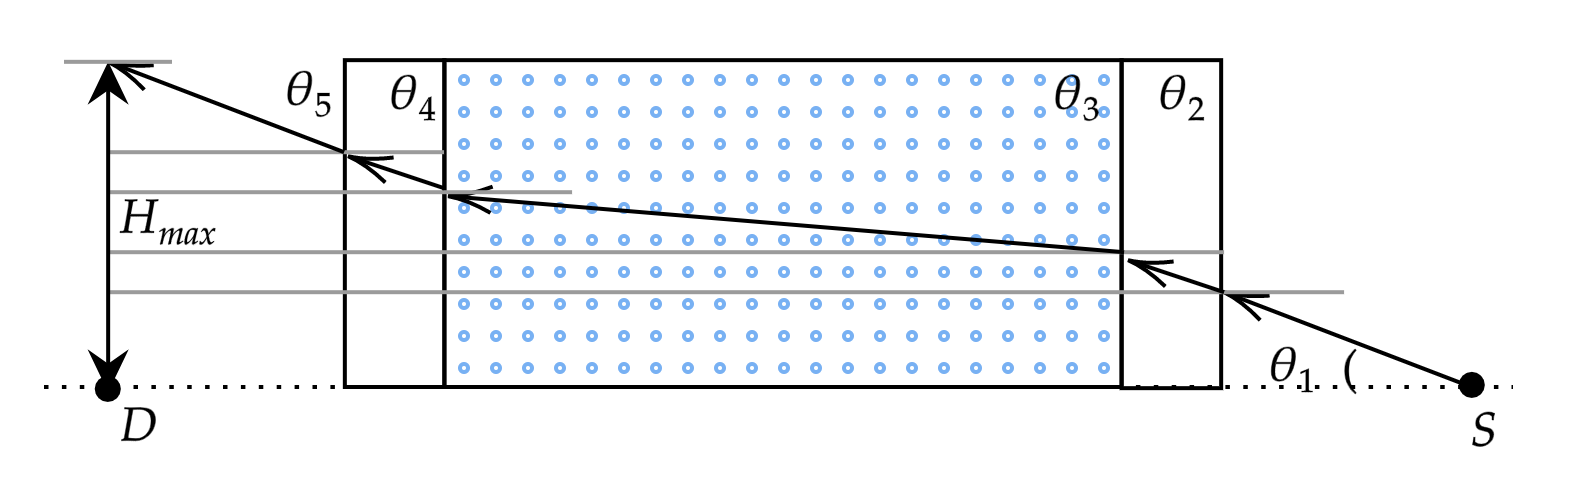
\includegraphics[width=0.75\textwidth]{chapter5/calculo distancia maxima de desviacion de haz de luz en condiciones ideales.png}
	\caption{Cálculo de distancia máxima de desviación de haz de luz en condiciones ideales.}
	\begin{myflushleftportland}
		Fuente: Elaboración propia.
	\end{myflushleftportland}
	\label{fig:calculo distancia maxima de desviacion de haz de luz en condiciones ideales}
\end{myfigure}

\begin{myequation}\label{eq:calculo distancia maxima de desviacion de haz de luz en condiciones ideales}
	\begin{split}
		H_{max}&=h_{1}+h_{2}+h_{3}+h_{4}+h_{5} \\
		H_{max}&=10*tan(\theta_{1})+3*tan(\theta_{2})+85*tan(\theta_{3})+3*tan(\theta_{4})+10*tan(\theta_{5}) \\
		H_{max}&=10*tan(5^\circ)+3*tan(3.33^\circ)+85*tan(3.76^\circ)+3*tan(3.33^\circ)+10*tan(5^\circ) \\
		H_{max}&=7.685 mm.
	\end{split}		
\end{myequation}

Para una óptima recepción se propone llegar como mínimo 75\% de haces de luz. Esto quiere decir que del diámetro ideal del dispositivo receptor debe ser de 15.4 mm y el óptimo 13.33 mm.\footnote{$d_{ideal-receptor}=2*H_{max}=15.4 mm.$ y $d_{75\%-receptor}=\sqrt{0.75*15.4^2}=13.33 mm.$ } Finalmente, los requerimientos mínimos que debe tener el sensor infrarrojo óptimo y comparaciones técnicas de los dispositivos comerciales que cumplen con los requerimientos se muestran en la Tabla \ref{tab:tabla comparativa de sensores infrarrojos}.

\begin{mytable}[H]
	\centering
	\caption{Tabla comparativa de sensores infrarrojos.}
	\label{tab:tabla comparativa de sensores infrarrojos}
	\begin{tabular}{l|c|c|c|c|}
		\cline{2-5}
		\multicolumn{1}{c|}{\textbf{}}            & \textbf{\begin{tabular}[c]{@{}c@{}}Requisitos\\ mínimos\end{tabular}} &
		\multicolumn{1}{|l|}{				
			\begin{minipage}{\mythirdmaxsizeofcontenttable}	
				\textbf{HD-DS25 CM-3MM}
			\end{minipage}
		}&
		\multicolumn{1}{|l|}{				
			\begin{minipage}{\mythirdmaxsizeofcontenttable}	
				\textbf{QT50CM}
			\end{minipage}
		}&
		\multicolumn{1}{|l|}{				
			\begin{minipage}{\mythirdmaxsizeofcontenttable}	
				\textbf{GP2Y0A 21YK0F}
			\end{minipage}
		}  \\ \hline
		\multicolumn{1}{|l|}{\textbf{Figura}} & - 
		&		  
		\begin{minipage}{\mythirdmaxsizeofcontenttable}
			\centering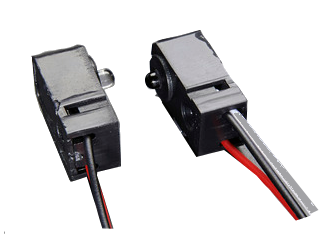
\includegraphics[width=\mythirdmaxsizeimageinsidetable]{chapter5/tablas comparativas/sensor infrarrojo 1.png} \\ 
			%\begin{myflushcenter}
			%	{\footnotesize Nombre imagen}
			%\end{myflushcenter}
		\end{minipage}
		&		  
		\begin{minipage}{\mythirdmaxsizeofcontenttable}
			\centering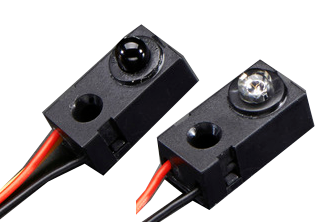
\includegraphics[width=\mythirdmaxsizeimageinsidetable]{chapter5/tablas comparativas/sensor infrarrojo 2.png} \\ 
			%\begin{myflushcenter}
			%	{\footnotesize Nombre imagen}
			%\end{myflushcenter}
		\end{minipage}
		&  
		\begin{minipage}{\mythirdmaxsizeofcontenttable}
			\centering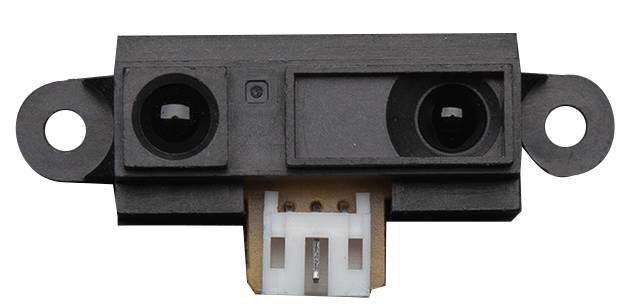
\includegraphics[width=\mythirdmaxsizeimageinsidetable]{chapter5/tablas comparativas/sensor infrarrojo 3.png} \\ 
			%\begin{myflushcenter}
			%	{\footnotesize Nombre imagen}
			%\end{myflushcenter}
		\end{minipage}\\ \hline
		\multicolumn{1}{|l|}{\textbf{Fabricante}} 
		& - & Adafruit & Adafruit & SHARP\\ \hline
		\multicolumn{1}{|l|}{
			\begin{minipage}{\myforthmaxsizeofcontenttable}	
				\textbf{Tipo de comunicación}
			\end{minipage}
		} & Digital & [0;VCC] & [0;VCC] & Analógico         \\ \hline
		\multicolumn{1}{|l|}{
			\begin{minipage}{\myforthmaxsizeofcontenttable}	
				\textbf{Área mínima circular de receptor ($mm^2$)}
			\end{minipage}
		} & 15.4 & 28.27 & 78.54 & 162.86         \\ \hline
		\multicolumn{1}{|l|}{
			\begin{minipage}{\myforthmaxsizeofcontenttable}	
				\textbf{Ángulo de visión/recepción (°)}
			\end{minipage}
		} & 5 & 10 & 10 & -         \\ \hline
		\multicolumn{1}{|l|}{
			\begin{minipage}{\myforthmaxsizeofcontenttable}	
				\textbf{Distancia de detección ($mm.$)}
			\end{minipage}
		} & 170 & [0;250] & [0;500] & [100;800] \\ \hline
		\multicolumn{1}{|l|}{
			\begin{minipage}{\myforthmaxsizeofcontenttable}	
				\textbf{Longitud de onda infrarroja recomendada ($nm$)}
			\end{minipage}
		} & 850 & - & - & 870$\pm$70 \\ \hline
		\multicolumn{1}{|l|}{
			\begin{minipage}{\myforthmaxsizeofcontenttable}	
				\textbf{Voltaje operativo VCC ($V$)}
			\end{minipage}
		} & 5  & [3.0;5.5] & [3.0;5.5] & [4.5;5.5]         \\ \hline
		\multicolumn{1}{|l|}{
			\begin{minipage}{\myforthmaxsizeofcontenttable}	
				\textbf{Consumo de corriente ($mA$)}
			\end{minipage}
		} & -  & 100 & 100 & 30         \\ \hline
		\multicolumn{1}{|l|}{
			\begin{minipage}{\myforthmaxsizeofcontenttable}	
				\textbf{Temperatura operativa (°$C$)}
			\end{minipage}
		} & [-10;60] & [-25;60] & [-25;60] & [-10;60] \\ \hline
		\multicolumn{1}{|l|}{
			\begin{minipage}{\myforthmaxsizeofcontenttable}	
				\textbf{Precio ($S/$)}
			\end{minipage}
		} & - & 7.00 & 23.32 & 53.68 \\ \hline
	\end{tabular}
	\begin{flushleft}	
		Fuente: Marktech Optoelectronics y elaboración propia. Hoja de datos técnico (\textit{Datasheet}) en el Anexo.\\
		Tasa de cambio de USD a PEN: S/ 3.59.
	\end{flushleft}
\end{mytable}

\textcolor{blue}{[BORRADOR] Seleccionar uno y explicar la selección [/BORRADOR]}

%% NUEVO SUBSECCION X.X.X.X
\subsubsection{Selección de cámaras} 

En el sistema se emplea dos cámaras con distintos requerimientos técnicos. Por un lado, una cámara estéreo se encarga de capturar imágenes que van a ser procesadas por algoritmos de detección y conteo de truchas. Por otro lado, una cámara normal registra la trayectoria de las truchas que en la distribución de estas a los canales de salida definidos por los algoritmos. 

\begin{itemize}
	
	\item \textbf{Cálculo de distancias apropiadas de las cámaras}
	
	El área que se debe captar sobre el proceso, sin las tuberías transparentes, se representan  en una vista frontal y de perfil en la Figura \ref{fig:distancia entre juego de espejos y camara estereo}. Donde: $d$ es la distancia entre el juego de espejos y la cámara, $\alpha$ es el HDFV\footnote{Campo de visión horizontal.}, $\beta$ es el VDFV\footnote{Campo de visión vertical.}, $A$ es la altura del área proyectada y $L$ es la largo del área proyectada del juego de espejos.
	
	\begin{myfigure}[H]
		\centering
		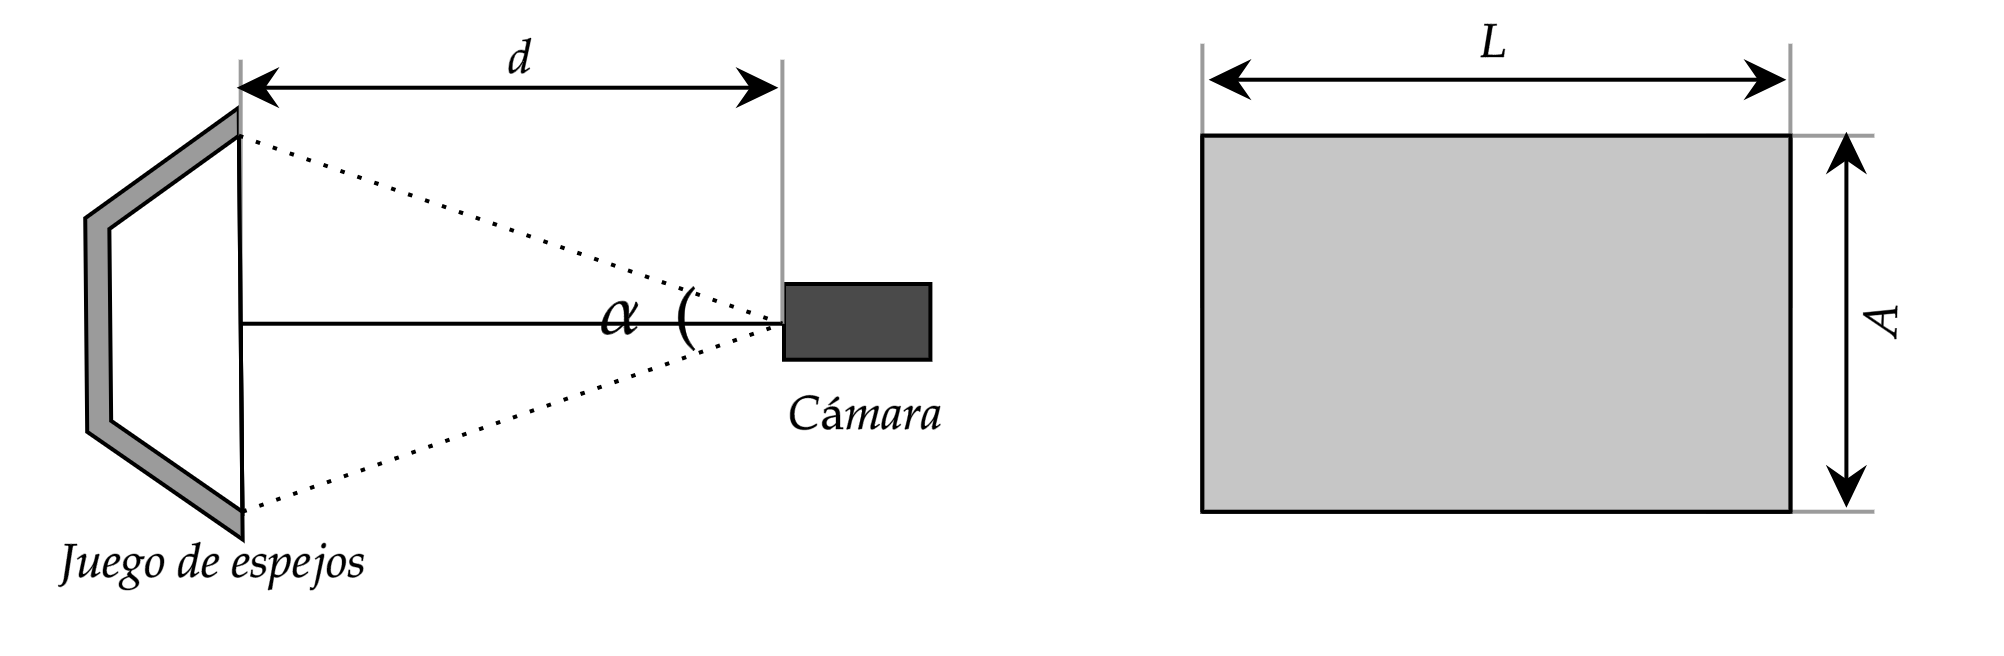
\includegraphics[width=1\textwidth]{chapter5/distancia entre juego de espejos y camara estereo.png}
		\caption{Distancia entre juego de espejos y cámara estéreo}
		\begin{myflushleftportland}
			Fuente: Elaboración propia.
		\end{myflushleftportland}
		\label{fig:distancia entre juego de espejos y camara estereo}
	\end{myfigure}

	De la geometría se obtiene los valores de $\alpha$ y $\beta$, que dependen de las otras variables. El posicionamiento de la cámara ($d$) estéreo estará sujeto a sus valores de HDFV y VDFV como se muestra en la Ecuación \ref{eq:calculo beta de distancia entre espejos y camara estereo} y \ref{eq:calculo alfa de distancia entre espejos y camara estereo}, respectivamente.
		
	\begin{myfigure}[H]
		\centering
		\includegraphics[width=1\textwidth]{chapter5/calculo de distancia entre espejos y camara estereo.png}
		\caption{Cálculo de distancia apropiada para la cámara estéreo}
		\begin{myflushleftportland}
			Fuente: Elaboración propia.
		\end{myflushleftportland}
		\label{fig:calculo de distancia entre espejos y camara estereo}
	\end{myfigure}
	
	\begin{myequation}\label{eq:calculo alfa de distancia entre espejos y camara estereo}
		\begin{split}
			tan(\alpha_{min}/2)&=\frac{A/2}{d}\\
			\alpha_{min}&=2*atan(\frac{A}{2*d})\\
		\end{split}		
	\end{myequation}

	\begin{myequation}\label{eq:calculo beta de distancia entre espejos y camara estereo}
		\begin{split}
			tan(\beta_{min}/2)&=\frac{L/2}{d}\\
			\beta_{min}&=2*atan(\frac{L}{2*d})\\
		\end{split}		
	\end{myequation}

	\item \textbf{Cálculo de cuadros por segundo (fps) necesarios para la cámara estéreo}
	
	\textcolor{blue}{[BORRADOR] Agregar descripción [/BORRADOR]}
	
	\begin{myfigure}[H]
		\centering
		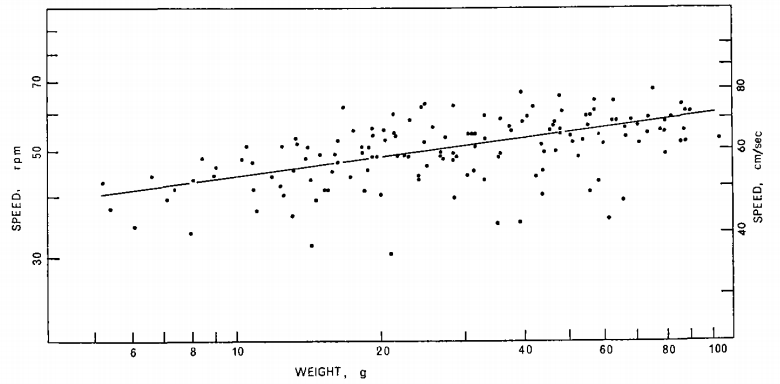
\includegraphics[width=1\textwidth]{chapter5/grafica tamano y velocidad de nado trucha arcoiris.png}
		\caption{Aproximación lineal de la relación entre peso y la velocidad de nado de truchas arcoíris}
		\begin{myflushleftportland}
			Fuente: \cite{Fry1970}
		\end{myflushleftportland}
		\label{fig:grafica tamano y velocidad de nado trucha arcoiris}
	\end{myfigure}
	
	
	En la Ecuación \ref{eq:ecuacion relacion tamano y velocidad de nado de trucha arcoiris} se muestra la relación entre \textit{X: peso de la trucha ($g$)} e \textit{Y: velocidad de nado ($cm/s$)} con un error \textit{Z= $\pm 0.033$}. 
	
	\begin{myequation} \label{eq:ecuacion relacion tamano y velocidad de nado de trucha arcoiris}
		Y=-3.965+2.908(Z)X
	\end{myequation}
	
	En el caso de este trabajo, la dimensión máxima y mínima de las truchas arcoíris son de 20 cm y 15 cm, respectivamente. De la Tabla \textit{Clasificación de truchas por etapas de producción}\footnote{\cite{DiazVergara2020}} podemos obtener los gramos mediante interpolación lineal para cada límite: valores mínimo-máximo son 153 y 199 \textit{$g$}, respectivamente. Utilizando los valores antes indicados y empleando la Ecuación \ref{eq:ecuacion relacion tamano y velocidad de nado de trucha arcoiris} obtenemos los valores límites dentro del rango $[10.71; 15.13] (cm/s)$. Luego de escoger la máxima velocidad con redondeo hacia arriba $v_{max}=16cm/s$), \textcolor{blue}{[BORRADOR] Falta explicación [/BORRADOR]}
	
	\item \textbf{Selección de cámara estéreo}
	
	El objetivo de la cámara estéreo es la de obtener fotos por determinado periodo de tiempo designado por los algoritmos de procesamiento de imágenes. Con el fin de cumplir el objetivo mencionado deben cumplirse requerimientos técnicos: fotografiar a la trucha con un enfoque aceptable que permita distinguir a la trucha adecuadamente, ángulo de visión horizontal y vertical, resolución, entre otros. En la Figura \ref{fig:diagrama esquematico camara estereo y dependencia de la distancia del objeto} se visualiza un diagrama referencial de una cámara estéreo, con la cuál podemos obtener distancias a partir de dos imágenes. 
	
	\begin{myfigure}[H]
		\centering
		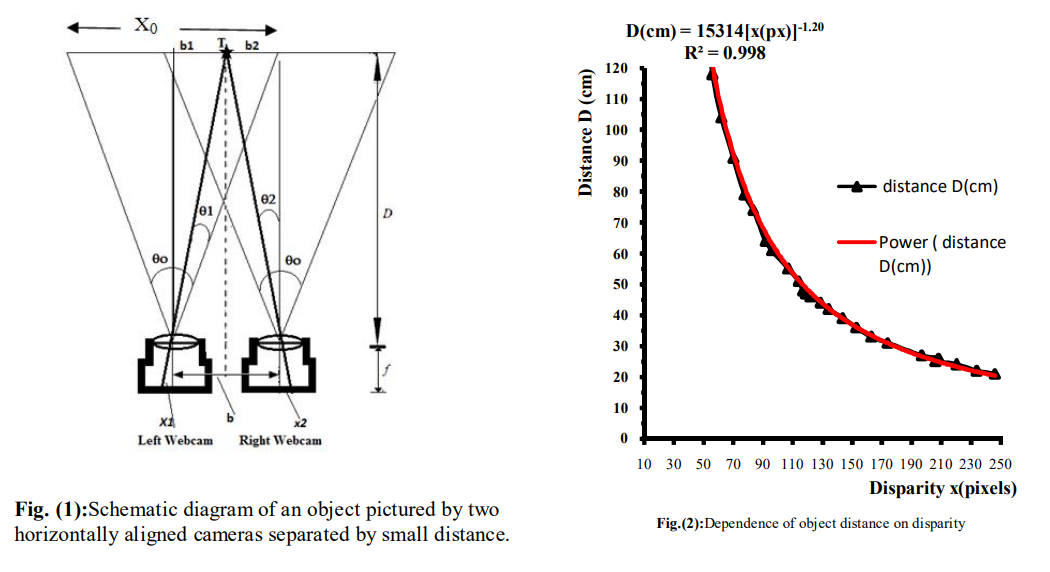
\includegraphics[width=1\textwidth]{chapter5/diagrama esquematico camara estereo y dependencia de la distancia del objeto.png}
		\caption[Diagrama esquemático y dependencia de la distancia del objeto seguido por una cámara estéreo.]{(Izq.) Diagrama esquemático de un objeto representado por dos cámaras alineadas horizontalmente separadas por una pequeña distancia. (Der.) Dependencia de la distancia del objeto en la disparidad.}
		\begin{myflushleftportland}
			Fuente: \cite{Mahammed2013}
		\end{myflushleftportland}
		\label{fig:diagrama esquematico camara estereo y dependencia de la distancia del objeto}
	\end{myfigure}

	\textcolor{blue}{[BORRADOR] Falta explicación [/BORRADOR]}
	
	Por ejemplo, el error realizado en pruebas con vehículos autónomos brindado en \cite{Zaarane2020} se muestra en la Figura \ref{fig:medicion de distancia con distintas distancias}. 
	
	\begin{myfigure}[H]
		\centering
		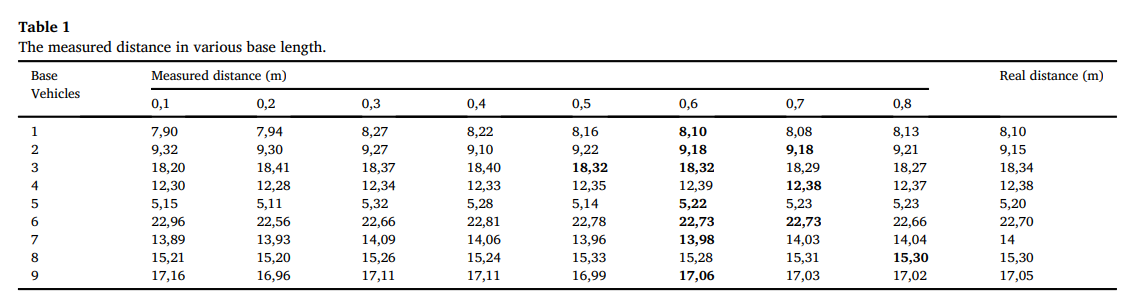
\includegraphics[width=1\textwidth]{chapter5/medicion de distancia con distintas distancias.png}
		\caption{Pruebas de medición con distintas distancias al objeto.}
		\begin{myflushleftportland}
			Fuente: \cite{Zaarane2020}
		\end{myflushleftportland}
		\label{fig:medicion de distancia con distintas distancias}
	\end{myfigure}
		
	%- Tamaño de píxeles requerido \\
	%- Cantidad de frames (80 fps con 3-4L/s) (Falta calcular con lo que hemos calculado 16 cm/s) \\ 
	%- La inclinación hace que el pez no tenga velocidad hacia arriba \\

	
	En la Tabla \ref{tab:tabla comparativa de camaras estereo} se muestra tanto los requerimientos mínimos como las cámaras estéreo candidatas para el sistema. El cálculo mencionado en la sección anterior se calcula luego de escoger una de entre las tres opciones mostradas.
	
	\begin{savenotes}
	\begin{mytable}[H]
		\centering
		\caption{Tabla comparativa de cámaras estéreo.}
		\label{tab:tabla comparativa de camaras estereo}
		\begin{tabular}{l|c|c|c|c|}
			\cline{2-5}
			\multicolumn{1}{c|}{\textbf{}}            & \textbf{\begin{tabular}[c]{@{}c@{}}Requisitos\\ mínimos\end{tabular}} & 
			\multicolumn{1}{|l|}{				
				\begin{minipage}{\mythirdmaxsizeofcontenttable}
					\begin{myflushcenter}
						\textbf{OAK-D}
					\end{myflushcenter}
				\end{minipage}
			}&
			\multicolumn{1}{|l|}{				
				\begin{minipage}{\mythirdmaxsizeofcontenttable}	
					\begin{myflushcenter}
						\textbf{B0263}
					\end{myflushcenter}
				\end{minipage}
			}&
			\multicolumn{1}{|l|}{				
				\begin{minipage}{\mythirdmaxsizeofcontenttable}	
					\begin{myflushcenter}
						\textbf{B0204}
					\end{myflushcenter}
				\end{minipage}
			}  \\ \hline
			\multicolumn{1}{|l|}{\textbf{Figura}} & - 
			&		  
			\begin{minipage}{\mythirdmaxsizeofcontenttable}
				\centering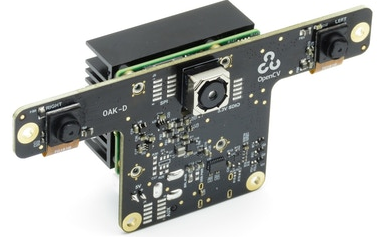
\includegraphics[width=\mythirdmaxsizeimageinsidetable]{chapter5/tablas comparativas/camara estereo 1.png} \\ 
				%\begin{myflushcenter}
				%	{\footnotesize Nombre imagen}
				%\end{myflushcenter}
			\end{minipage}
			&		  
			\begin{minipage}{\mythirdmaxsizeofcontenttable}
				\centering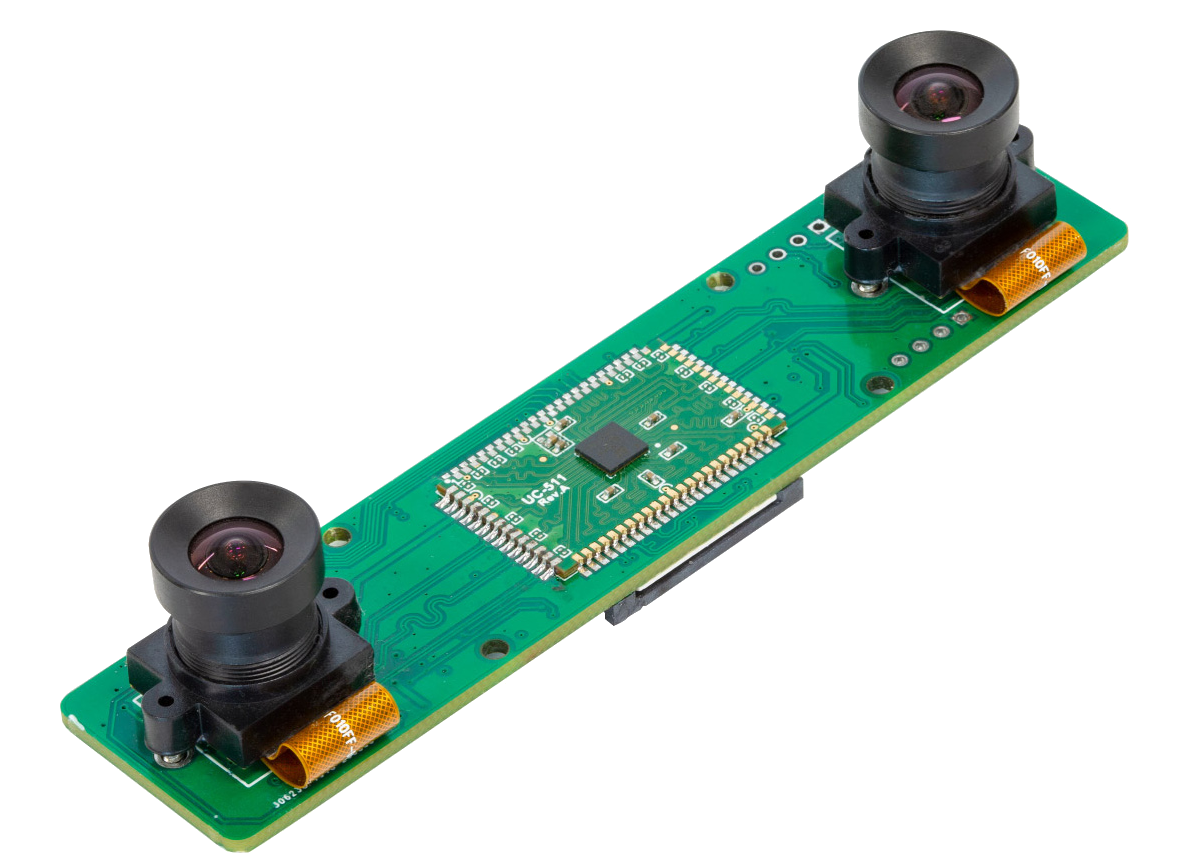
\includegraphics[width=\mythirdmaxsizeimageinsidetable]{chapter5/tablas comparativas/camara estereo 2.png} \\ 
				%\begin{myflushcenter}
				%	{\footnotesize Nombre imagen}
				%\end{myflushcenter}
			\end{minipage}
			&  
			\begin{minipage}{\mythirdmaxsizeofcontenttable}
				\centering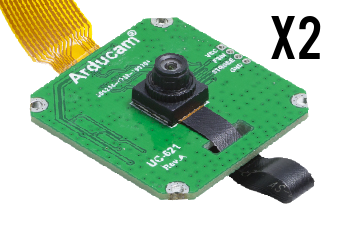
\includegraphics[width=\mythirdmaxsizeimageinsidetable]{chapter5/tablas comparativas/camara estereo 3.png} \\ 
				%\begin{myflushcenter}
				%	{\footnotesize Nombre imagen}
				%\end{myflushcenter}
			\end{minipage}\\ \hline
			\multicolumn{1}{|l|}{
				\begin{minipage}{\myforthmaxsizeofcontenttable}	
					\textbf{Fabricante}
				\end{minipage}
			} & - & OpenCV & ArduCam & ArduCam \\ \hline
			\multicolumn{1}{|l|}{
				\begin{minipage}{\myforthmaxsizeofcontenttable}	
					\textbf{Sensor óptico}
				\end{minipage}
			} & - & OV9282 & OV9281 & OV2311 \\ \hline
			\multicolumn{1}{|l|}{
				\begin{minipage}{\myforthmaxsizeofcontenttable}	
					\textbf{Tipo de obturador}
				\end{minipage}
			} & 
			\begin{minipage}{\mythirdmaxsizeofcontenttable}\begin{myflushcenter}
				Global sincronizado 
			\end{myflushcenter}\end{minipage} & 
			\begin{minipage}{\mythirdmaxsizeofcontenttable}\begin{myflushcenter}
				Global sincronizado 
			\end{myflushcenter}\end{minipage} &
			\begin{minipage}{\mythirdmaxsizeofcontenttable}\begin{myflushcenter}
				Global sincronizado 
			\end{myflushcenter}\end{minipage}&
			\begin{minipage}{\mythirdmaxsizeofcontenttable}\begin{myflushcenter}
				Global dual 
			\end{myflushcenter}\end{minipage} \\ \hline
			\multicolumn{1}{|l|}{
				\begin{minipage}{\myforthmaxsizeofcontenttable}	
					\textbf{Escala de colores}
				\end{minipage}
			} & - & RGB & B/N & B/N \\ \hline
			\multicolumn{1}{|l|}{
				\begin{minipage}{\myforthmaxsizeofcontenttable}	
					\textbf{Resolución}
				\end{minipage}
			} & 0.5MP & 
			\begin{minipage}{\mythirdmaxsizeofcontenttable}\begin{myflushcenter}
					1MP (1280× 800 $px/3{\mu}m$)
			\end{myflushcenter}\end{minipage} & 
			\begin{minipage}{\mythirdmaxsizeofcontenttable}\begin{myflushcenter}
					1MP (1280× 800 $px/3{\mu}m$)
			\end{myflushcenter}\end{minipage} & 
			\begin{minipage}{\mythirdmaxsizeofcontenttable}\begin{myflushcenter}
					2MP (1600x 1300 $px/3{\mu}m$)
			\end{myflushcenter}\end{minipage} \\ \hline
			\multicolumn{1}{|l|}{
				\begin{minipage}{\myforthmaxsizeofcontenttable}	
					\textbf{Frames por segundo ($FPS$)}
				\end{minipage}
			} & 60 % NECESITO MÁS DE 80
			& 120 & 60 & 60 \\ \hline
			\multicolumn{1}{|l|}{
				\begin{minipage}{\myforthmaxsizeofcontenttable}	
					\textbf{Tamaño de lente ('')}
				\end{minipage}
			} & Independiente & 1/2.3 & 1/4 & 1/2.9 \\ \hline
			\multicolumn{1}{|l|}{
				\begin{minipage}{\myforthmaxsizeofcontenttable}	
					\textbf{Enfoque ($mm.$)}
				\end{minipage}
			} & - & [196;$\infty$] & [30;$\infty$] & [30;$\infty$] \\ \hline
			\multicolumn{1}{|l|}{
				\begin{minipage}{\myforthmaxsizeofcontenttable}
					\textbf{Campo de visión ° (HFDV,VFDV,DFDV)\footnote{HFDV: Campo de visión horizontal. VFDV: Campo de visión vertical. DFDV: Campo de visión diagonal}}
				\end{minipage}
			} & Adaptable & 71.8, --, 81.0 & 70, 52.1 , -- & 100, 68.2, -- \\ \hline
			\multicolumn{1}{|l|}{
				\begin{minipage}{\myforthmaxsizeofcontenttable}	
					\textbf{Procesamiento gráfico}
				\end{minipage}
			} & - & MA2085 VPU\footnote{Movidius™ Myriad™ VPU. \href{https://www.intel.com/content/www/us/en/products/processors/movidius-vpu/movidius-myriad-x.html}{Enlace a unidad de procesamiento de visión.}} & 
			\begin{minipage}{\mythirdmaxsizeofcontenttable}\begin{myflushcenter}
				Jetson Nano o Xavier NX
			\end{myflushcenter}\end{minipage}
		 	& \begin{minipage}{\mythirdmaxsizeofcontenttable}\begin{myflushcenter}
		 			Raspberry Pi 3
		 	\end{myflushcenter}\end{minipage} \\ \hline 
		 	\multicolumn{1}{|l|}{
		 		\begin{minipage}{\myforthmaxsizeofcontenttable}	
		 			\textbf{Temperatura operativa}
		 		\end{minipage}
		 	} & [-10;50] & [-30;60] & [-30;85] & [-30;85] \\ \hline
			\multicolumn{1}{|l|}{
				\begin{minipage}{\myforthmaxsizeofcontenttable}	
					\textbf{Soporte IA\footnote{Chips diseñados y optimizados para procesar detección de objetos mediante redes neuronales.}}
				\end{minipage}
			} & - & Sí & Sí & No \\ \hline
			\multicolumn{1}{|l|}{
				\begin{minipage}{\myforthmaxsizeofcontenttable}	
					\textbf{Consumo de energía ($W$)}
				\end{minipage}
			} & <10 & $\approx4$ & - & - \\ \hline
			\multicolumn{1}{|l|}{
				\begin{minipage}{\myforthmaxsizeofcontenttable}	
					\textbf{Precio (S/)}
				\end{minipage}
			} & <1000 & 475.41 & 358.97 & 717.28 \\ \hline
		\end{tabular}
		\begin{flushleft}	
			Fuente: OpenCV, ArduCam y elaboración propia. Hoja de datos técnico (\textit{Datasheet}) en el Anexo.\\
			Tasa de cambio de USD a PEN: S/ 3.59.
		\end{flushleft}
	\end{mytable}
	\end{savenotes}
	
	\textcolor{blue}{[BORRADOR] Decicisión de qué actuador será escogido y por qué en base a las características mencionadas [/BORRADOR]}
	
	\item \textbf{Selección de cámara simple}
	
	La cámara simple tiene como función verificar la correcta trayectoria de las truchas en el mecanismo de distribución hacia las respectivas jaulas flotantes. Los requerimientos técnicos se presentan en la Tabla \ref{tab:tabla comparativa de camaras simples} así como las principales características de cada una.
	
	\begin{savenotes}
		\begin{mytable}[H]
			\centering
			\caption{Tabla comparativa de cámaras.}
			\label{tab:tabla comparativa de camaras simples}
			\begin{tabular}{l|c|c|c|c|}
				\cline{2-5}
				\multicolumn{1}{c|}{\textbf{}}            & \textbf{\begin{tabular}[c]{@{}c@{}}Requisitos\\ mínimos\end{tabular}} & 
				\multicolumn{1}{|l|}{				
					\begin{minipage}{\mythirdmaxsizeofcontenttable}
						\begin{myflushcenter}
							\textbf{B0249}
						\end{myflushcenter}
					\end{minipage}
				}&
				\multicolumn{1}{|l|}{				
					\begin{minipage}{\mythirdmaxsizeofcontenttable}	
						\begin{myflushcenter}
							\textbf{Alvium 1800 U-500m}
						\end{myflushcenter}
					\end{minipage}
				}&
				%\multicolumn{1}{|l|}{				
				%	\begin{minipage}{\mythirdmaxsizeofcontenttable}	
				%		\begin{myflushcenter}
				%			\textbf{CMT-8MP- IMX219M366}
				%		\end{myflushcenter}
				%	\end{minipage}
				%}  
				\multicolumn{1}{|l|}{				
					\begin{minipage}{\mythirdmaxsizeofcontenttable}	
						\begin{myflushcenter}
							\textbf{OAK-1}
						\end{myflushcenter}
					\end{minipage}
				}  \\ \hline
				\multicolumn{1}{|l|}{\textbf{Figura}} & - 
				&		  
				\begin{minipage}{\mythirdmaxsizeofcontenttable}
					\centering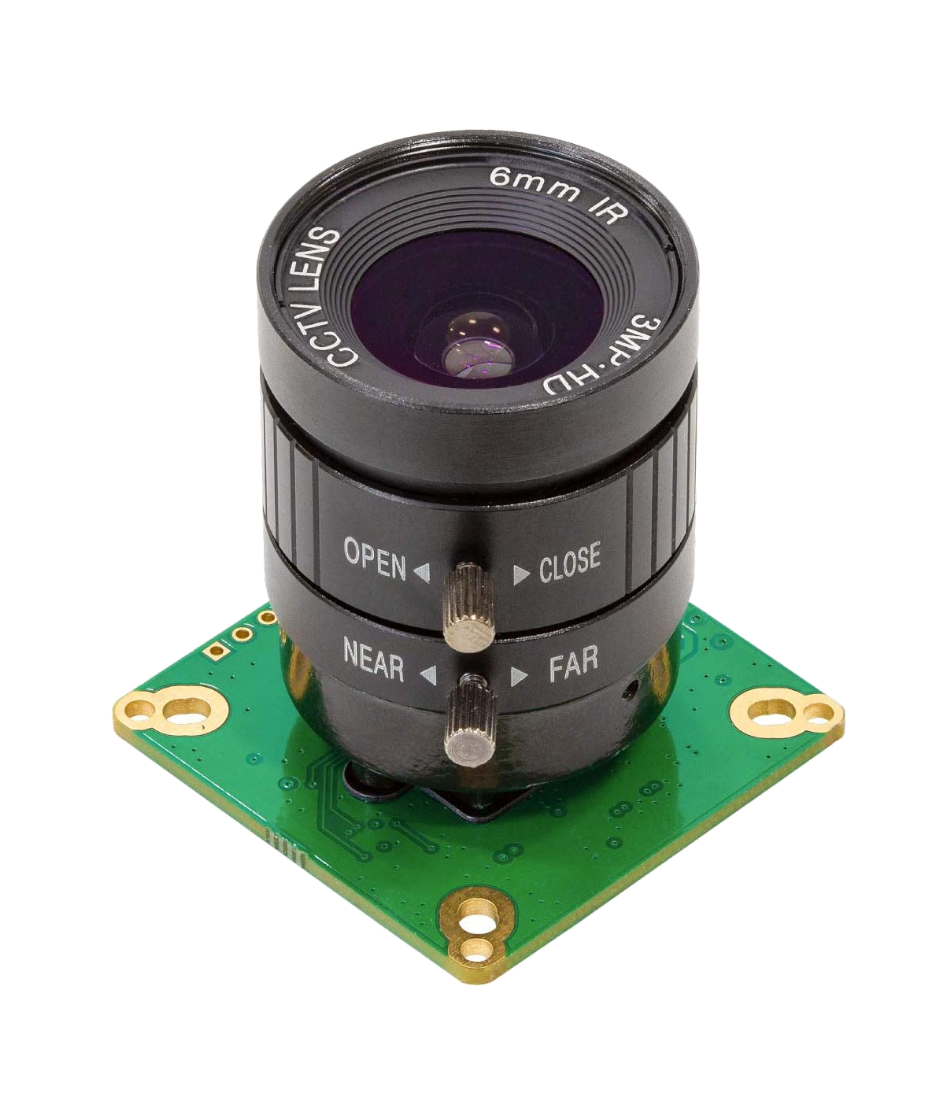
\includegraphics[width=\mythirdmaxsizeimageinsidetable]{chapter5/tablas comparativas/camara simple 1.png} \\ 
					%\begin{myflushcenter}
					%	{\footnotesize Nombre imagen}
					%\end{myflushcenter}
				\end{minipage}
				&		  
				\begin{minipage}{\mythirdmaxsizeofcontenttable}
					\centering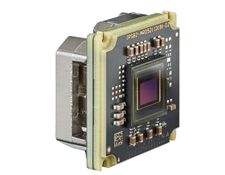
\includegraphics[width=\mythirdmaxsizeimageinsidetable]{chapter5/tablas comparativas/camara simple 2.png} \\ 
					%\begin{myflushcenter}
					%	{\footnotesize Nombre imagen}
					%\end{myflushcenter}
				\end{minipage}
				&  
				\begin{minipage}{\mythirdmaxsizeofcontenttable}
					\centering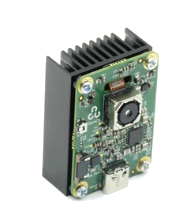
\includegraphics[width=\mythirdmaxsizeimageinsidetable]{chapter5/tablas comparativas/camara simple 4.png} \\ 
					%\begin{myflushcenter}
					%	{\footnotesize Nombre imagen}
					%\end{myflushcenter}
				\end{minipage}\\ \hline
				\multicolumn{1}{|l|}{
					\begin{minipage}{\myforthmaxsizeofcontenttable}	
						\textbf{Fabricante}
					\end{minipage}
				} & - & ArduCam & Allied Vision & ArduCam \\ \hline
				\multicolumn{1}{|l|}{
					\begin{minipage}{\myforthmaxsizeofcontenttable}	
						\textbf{Sensor óptico}
					\end{minipage}
				} & - & IMX477  & 
				\begin{minipage}{\mythirdmaxsizeofcontenttable}\begin{myflushcenter}
						ON Semi AR0521SR
				\end{myflushcenter}\end{minipage} & 
				%IMX219 
				IMX378
				\\ \hline
				\multicolumn{1}{|l|}{
					\begin{minipage}{\myforthmaxsizeofcontenttable}	
						\textbf{Tipo de obturador}
					\end{minipage}
				} & 
				\begin{minipage}{\mythirdmaxsizeofcontenttable}\begin{myflushcenter}
						- 
				\end{myflushcenter}\end{minipage} & 
				\begin{minipage}{\mythirdmaxsizeofcontenttable}\begin{myflushcenter}
						Global
				\end{myflushcenter}\end{minipage} &
				\begin{minipage}{\mythirdmaxsizeofcontenttable}\begin{myflushcenter}
						Rolling 
				\end{myflushcenter}\end{minipage}&
				%\begin{minipage}{\mythirdmaxsizeofcontenttable}\begin{myflushcenter}
				%		Rolling 
				%\end{myflushcenter}\end{minipage} 
				\begin{minipage}{\mythirdmaxsizeofcontenttable}\begin{myflushcenter}
					Global 
				\end{myflushcenter}\end{minipage} 			
				\\ \hline
				\multicolumn{1}{|l|}{
					\begin{minipage}{\myforthmaxsizeofcontenttable}	
						\textbf{Escala de colores}
					\end{minipage}
				} & - & RGB & B/N & RGB \\ \hline
				\multicolumn{1}{|l|}{
				\begin{minipage}{\myforthmaxsizeofcontenttable}	
					\textbf{Resolución}
				\end{minipage}
				} & 0.5MP & 
				\begin{minipage}{\mythirdmaxsizeofcontenttable}\begin{myflushcenter}
					12.3MP (4056× 3040 $px/1.55{\mu}m$)
				\end{myflushcenter}\end{minipage} & 
				\begin{minipage}{\mythirdmaxsizeofcontenttable}\begin{myflushcenter}
					5MP (2592x 1944 $px/2.2{\mu}m$)
				\end{myflushcenter}\end{minipage} & 
				%\begin{minipage}{\mythirdmaxsizeofcontenttable}\begin{myflushcenter}
				%	8MP (3280x 2464 $px/1.12{\mu}m$)
				%\end{myflushcenter}\end{minipage} 
				\begin{minipage}{\mythirdmaxsizeofcontenttable}\begin{myflushcenter}
					12MP (4056× 3040 $px/1.55{\mu}m$)
				\end{myflushcenter}\end{minipage} 
				\\ \hline
				\multicolumn{1}{|l|}{
				\begin{minipage}{\myforthmaxsizeofcontenttable}	
					\textbf{Frames por segundo ($FPS$)}
				\end{minipage}
				} & 40 % NECESITO MÁS DE 80
				& 60 & 67 & 
				%720p60 
				60
				\\ \hline
				\multicolumn{1}{|l|}{
				\begin{minipage}{\myforthmaxsizeofcontenttable}	
					\textbf{Tamaño de lente ('')}
				\end{minipage}
				} & Independiente & 1/2.3 & 1/2.5 &
				% 1/4
				1/2.3
				\\ \hline
				\multicolumn{1}{|l|}{
				\begin{minipage}{\myforthmaxsizeofcontenttable}
					\textbf{Campo de visión ° (HFDV,VFDV,DFDV)\footnote{HFDV: Campo de visión horizontal. VFDV: Campo de visión vertical. DFDV: Campo de visión diagonal}}
				\end{minipage}
				} & Adaptable & 65.0, --, -- & -- & 
				%70, 70, -- 
				71.8, --, 81.0
				\\ \hline
				\multicolumn{1}{|l|}{
				\begin{minipage}{\myforthmaxsizeofcontenttable}	
					\textbf{Procesamiento gráfico}
				\end{minipage}
				} & - & 
				\begin{minipage}{\mythirdmaxsizeofcontenttable}\begin{myflushcenter}
					Jetson Nano o Xavier NX
				\end{myflushcenter}\end{minipage} & 
				\begin{minipage}{\mythirdmaxsizeofcontenttable}\begin{myflushcenter}
					Jetson Nano o Xavier NX
				\end{myflushcenter}\end{minipage}&
				%\begin{minipage}{\mythirdmaxsizeofcontenttable}\begin{myflushcenter}
				%	Raspberry Pi 3
				%\end{myflushcenter}\end{minipage}
				\begin{minipage}{\mythirdmaxsizeofcontenttable}\begin{myflushcenter}
					MA2085 VPU\footnote{Movidius™ Myriad™ VPU. \href{https://www.intel.com/content/www/us/en/products/processors/movidius-vpu/movidius-myriad-x.html}{Enlace a unidad de procesamiento de visión.}}
				\end{myflushcenter}\end{minipage}  \\ \hline 
				\multicolumn{1}{|l|}{
				\begin{minipage}{\myforthmaxsizeofcontenttable}	
					\textbf{Temperatura operativa}
				\end{minipage}
				} & [-10;50] & [-20;60] & [5;80] & 
				%[-20;70]
	            [-30;60]
	            \\ \hline
				\multicolumn{1}{|l|}{
				\begin{minipage}{\myforthmaxsizeofcontenttable}	
					\textbf{Consumo de energía ($W$)}
				\end{minipage}
				} & <5 & - & [$\approx$2.2;$\approx$2.4] & 
				%- 
				$\approx$2
				\\ \hline
				\multicolumn{1}{|l|}{
				\begin{minipage}{\myforthmaxsizeofcontenttable}	
					\textbf{Precio (S/)}
				\end{minipage}
				} & <500 & 196.81 & 595.7 & %717.28 
				355.41
				\\ \hline
				\end{tabular}
			\begin{flushleft}	
				Fuente: Allied Vision, ArduCam y elaboración propia. Hoja de datos técnico (\textit{Datasheet}) en el Anexo.\\
				Tasa de cambio de USD a PEN: S/ 3.59.
			\end{flushleft}
		\end{mytable}
	\end{savenotes}
	
	\textcolor{blue}{[BORRADOR] Decicisión de qué cámara será escogida y por qué, en base a las características mencionadas [/BORRADOR]}
	
\end{itemize}

%% NUEVO SUBSECCION X.X.X.X
\subsubsection{Selección de iluminación adecuada} 

\textcolor{blue}{[BORRADOR] Explicar. [/BORRADOR]}

%% NUEVO SUBSECCION X.X.X.X
\subsubsection{Selección de led de alta potencia}

El propósito de los leds de alta potencia es iluminar la zona en la que se realiza la captura de imágenes para detectar truchas y procesarlas. El uso de una led adecuado puede mejorar el rendimiento de la cámara. En la Figura \ref{fig:iluminacion opciones} se muestra las opciones de iluminación que se consideraron, resultando el uso de dos tiras de leds adecuadas para el sistema.

% EN LA CARPETA IMAGENES ESTAN TODA LAS IMAGENES BASE
\begin{myfigure}[H]
	\centering
	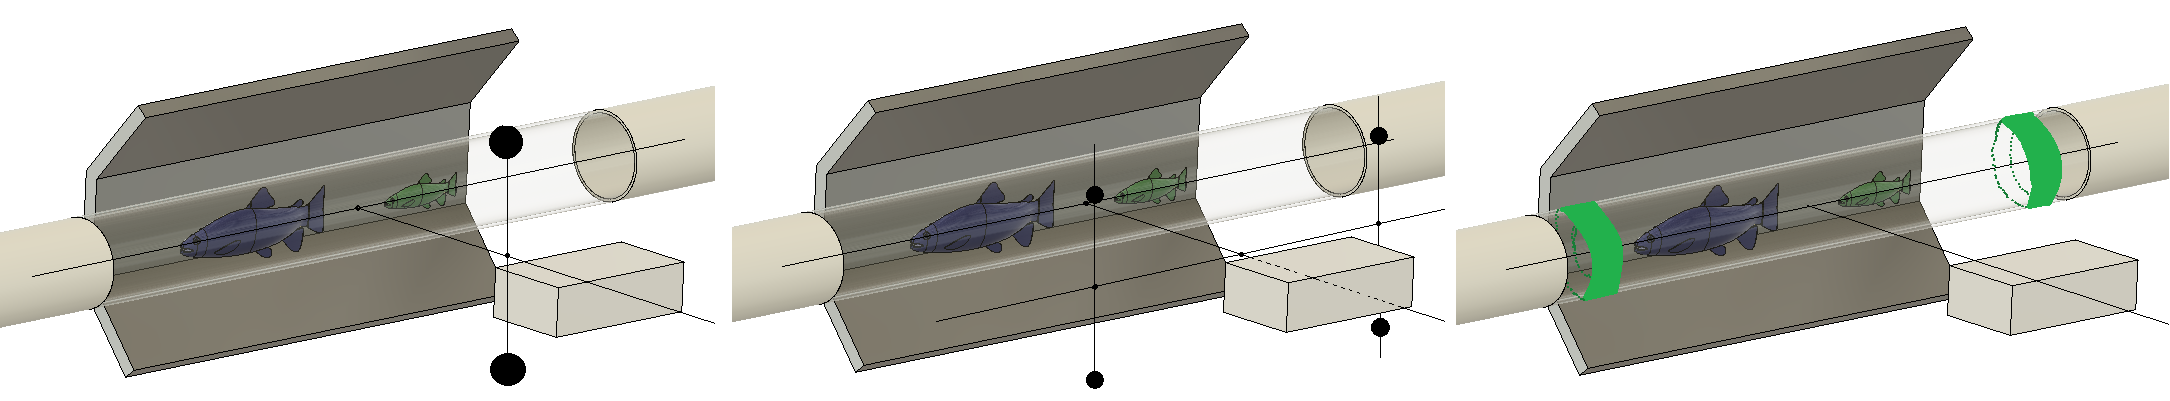
\includegraphics[width=1\textwidth]{chapter5/iluminacion opciones.png}
	\caption[Opciones de posicionamiento de iluminación.]{(Izq.) Iluminación con dos leds frente al sistema. (Cen.) Iluminación con cuatro leds frente al sistema. (Der.) Iluminación con dos tiras leds.}
	\begin{myflushleftportland}
		Fuente: Elaboración propia.
	\end{myflushleftportland}
	\label{fig:iluminacion opciones}
\end{myfigure}


La selección de una iluminación adecuada es tan importante como la selección de los otros componentes del subsistema: la ausencia de una iluminación adecuada puede degradar el rendimiento de los algoritmos, así como los de obtención de fotografías en la cámara estéreo debido al tiempo de exposición necesario por fotografía.

\begin{myequation}\label{eq:calculo de led de alta potencia}
	\begin{split}
		Iluminación_{necesaria}&=1000 %(lumenes)
	\end{split}		
\end{myequation}

\textcolor{blue}{[BORRADOR] Encontrar referencias bibliográficas de valores de iluminación adecuadas para este propósito. [/BORRADOR]}

En la Tabla \ref{tab:tabla comparativa de leds de alta potencia} se muestra una tabla técnica comparativa. \textcolor{blue}{[BORRADOR] Introducción para la tabla [/BORRADOR]}

\begin{savenotes}
	\begin{mytable}[H]
		\centering
		\caption{Tabla comparativa de leds de alta potencia.}
		\label{tab:tabla comparativa de leds de alta potencia}
		\begin{tabular}{l|c|c|c|c|}
			\cline{2-5}
			\multicolumn{1}{c|}{\textbf{}}            & \textbf{\begin{tabular}[c]{@{}c@{}}Requisitos\\ mínimos\end{tabular}} & 
			\multicolumn{1}{|l|}{				
				\begin{minipage}{\mythirdmaxsizeofcontenttable}
					\begin{myflushcenter}
						\textbf{T1}
					\end{myflushcenter}
				\end{minipage}
			}&
			\multicolumn{1}{|l|}{				
				\begin{minipage}{\mythirdmaxsizeofcontenttable}	
					\begin{myflushcenter}
						\textbf{T2}
					\end{myflushcenter}
				\end{minipage}
			}&
			\multicolumn{1}{|l|}{				
				\begin{minipage}{\mythirdmaxsizeofcontenttable}	
					\begin{myflushcenter}
						\textbf{T3}
					\end{myflushcenter}
				\end{minipage}
			}  \\ \hline
			\multicolumn{1}{|l|}{\textbf{Figura}} & - 
			&		  
			\begin{minipage}{\mythirdmaxsizeofcontenttable}
				\centering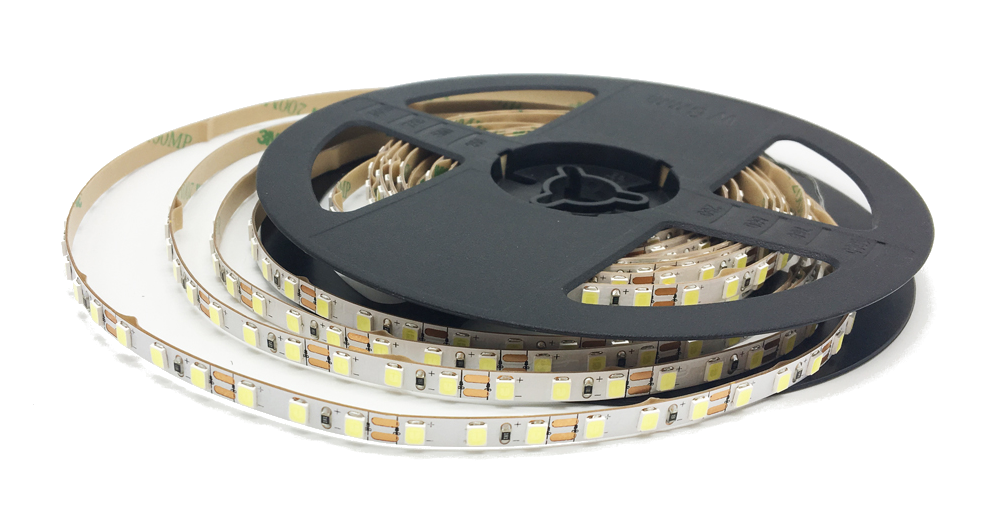
\includegraphics[width=\mythirdmaxsizeimageinsidetable]{chapter5/tablas comparativas/led alta potencia 1.png} \\ 
				%\begin{myflushcenter}
				%	{\footnotesize Nombre imagen}
				%\end{myflushcenter}
			\end{minipage}
			&		  
			\begin{minipage}{\mythirdmaxsizeofcontenttable}
				\centering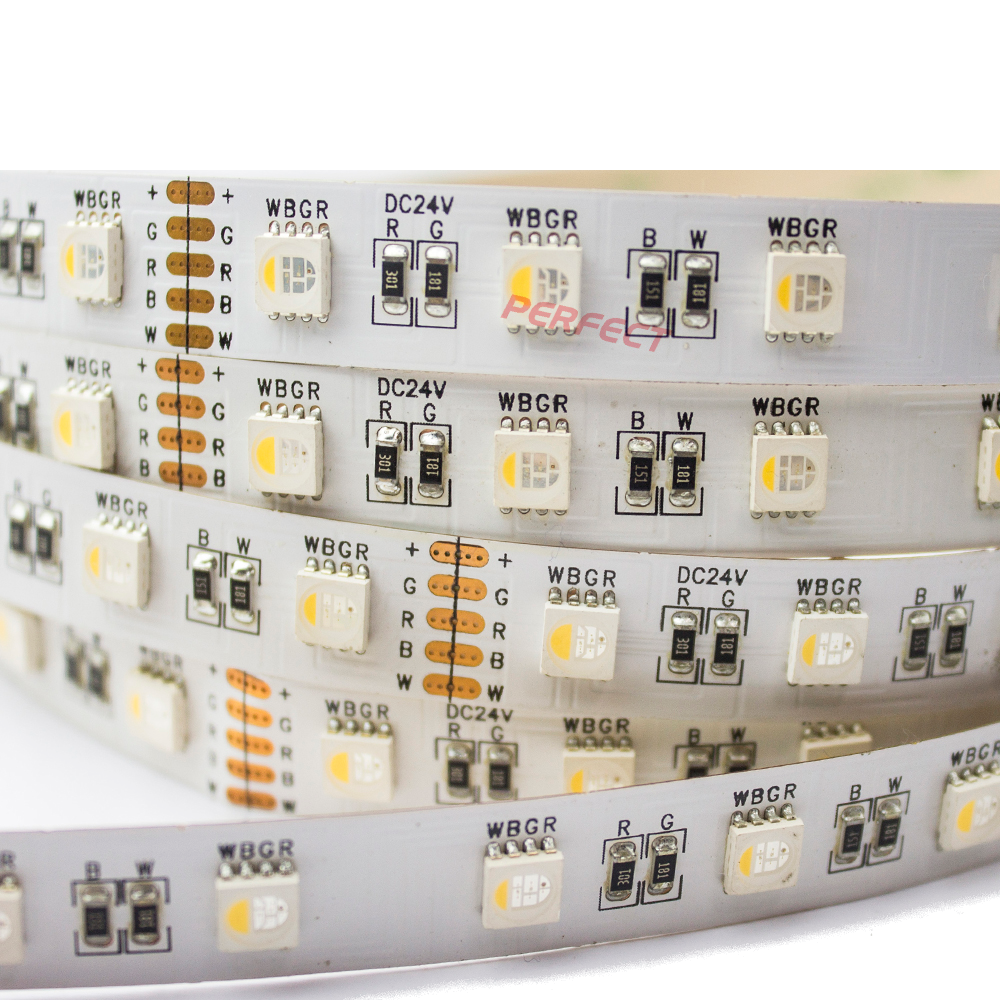
\includegraphics[width=\mythirdmaxsizeimageinsidetable]{chapter5/tablas comparativas/led alta potencia 2.png} \\ 
				%\begin{myflushcenter}
				%	{\footnotesize Nombre imagen}
				%\end{myflushcenter}
			\end{minipage}
			&  
			\begin{minipage}{\mythirdmaxsizeofcontenttable}
				\centering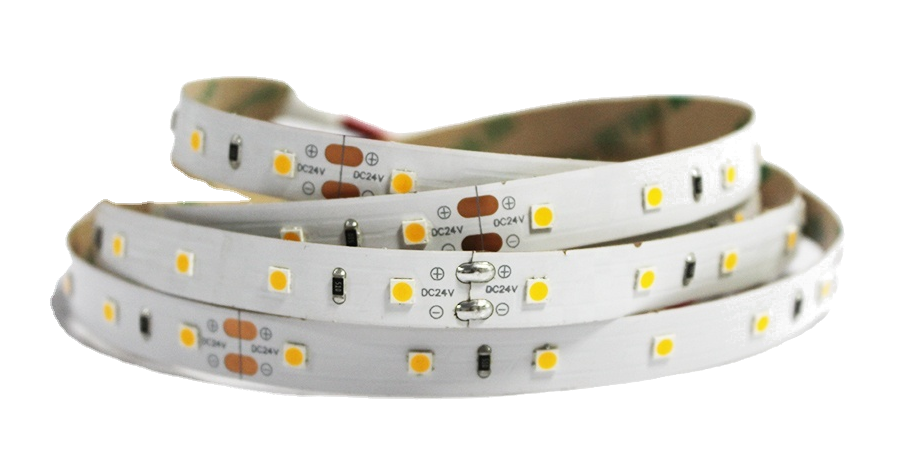
\includegraphics[width=\mythirdmaxsizeimageinsidetable]{chapter5/tablas comparativas/led alta potencia 3.png} \\ 
				%\begin{myflushcenter}
				%	{\footnotesize Nombre imagen}
				%\end{myflushcenter}
			\end{minipage}\\ \hline
			\multicolumn{1}{|l|}{
				\begin{minipage}{\myforthmaxsizeofcontenttable}	
					\textbf{Fabricante}
				\end{minipage}
			} & - & 12SAF4 & AFAS222 & ASFASF \\ \hline
			\multicolumn{1}{|l|}{
				\begin{minipage}{\myforthmaxsizeofcontenttable}	
					\textbf{ABC}
				\end{minipage}
			} & 
			\begin{minipage}{\mythirdmaxsizeofcontenttable}\begin{myflushcenter}
					- 
			\end{myflushcenter}\end{minipage} & 
			\begin{minipage}{\mythirdmaxsizeofcontenttable}\begin{myflushcenter}
					1
			\end{myflushcenter}\end{minipage} &
			\begin{minipage}{\mythirdmaxsizeofcontenttable}\begin{myflushcenter}
					2 
			\end{myflushcenter}\end{minipage}&
			\begin{minipage}{\mythirdmaxsizeofcontenttable}\begin{myflushcenter}
					3 
			\end{myflushcenter}\end{minipage} \\ \hline
		\end{tabular}
		\begin{flushleft}	
			Fuente: Imágenes de dominio público y elaboración propia. Hoja de datos técnico (\textit{Datasheet}) en el Anexo.\\
			Tasa de cambio de USD a PEN: S/ 3.59.
		\end{flushleft}
	\end{mytable}
\end{savenotes}

\textcolor{blue}{[BORRADOR] Decisión de qué LED será escogido y por qué, en base a las características mencionadas [/BORRADOR]}

%% NUEVO SUBSECCION X.X.X.X
\subsubsection{Selección de algoritmo de clasificación y conteo}
\label{sssec:seleccion de algoritmo de clasificacion y conteo}

Los algoritmos tienen como objetivo contar y clasificar truchas. \textcolor{red}{[BORRADOR] Explicar la necesidad de algoritmos. Explicar por qué algoritmos de detección CNN. [/BORRADOR]}

Los algoritmos de detección son evaluados en la Tabla \ref{tab:tabla comparativa de algoritmos} mediante una comparación técnica en cuanto a diversos puntos: \textcolor{blue}{[BORRADOR] tiempo de respuesta, costo de hardware requerido, consumo eléctrico del hardware, etc. [/BORRADOR]} 

\begin{savenotes}
	\begin{mytable}[H]
		\centering
		\caption{Tabla comparativa de algoritmos.}
		\label{tab:tabla comparativa de algoritmos}
		\begin{tabular}{l|c|c|c|c|c|c|c|}
			\cline{2-8}
			\multicolumn{1}{c|}{\textbf{}} &
			\textbf{\begin{tabular}[c]{@{}c@{}}Requisitos\\ mínimos\end{tabular}} &
			\textbf{1} &
			\textbf{2} &
			\textbf{3} &
			\textbf{1} &
			\textbf{2} &
			\textbf{3} \\ \hline
			\multicolumn{1}{|l|}{\textbf{Figura}}     & -  & 5  & 6  & 7  & 5  & 6  & 7  \\ \hline
			\multicolumn{1}{|l|}{\textbf{Fabricante}} & 8  & 9  & 10 & 11 & 9  & 10 & 11 \\ \hline
			\multicolumn{1}{|l|}{\textbf{A}}          & 12 & 13 & 14 & 15 & 13 & 14 & 15 \\ \hline
			\multicolumn{1}{|l|}{\textbf{B}}          & 16 & 17 & 18 & 19 & 17 & 18 & 19 \\ \hline
			\multicolumn{1}{|l|}{\textbf{C}}          & 20 & 21 & 22 & 23 & 21 & 22 & 23 \\ \hline
			\multicolumn{1}{|l|}{\textbf{D}}          & 24 & 25 & 26 & 27 & 25 & 26 & 27 \\ \hline
			\multicolumn{1}{|l|}{\textbf{E}}          & 32 & 33 & 34 & 35 & 33 & 34 & 35 \\ \hline
		\end{tabular}
		\begin{flushleft}	
			Fuente: Imágenes de dominio público y elaboración propia. \\
			Tasa de cambio de USD a PEN: S/ 3.59.
		\end{flushleft}
	\end{mytable}
\end{savenotes}

\textcolor{red}{[BORRADOR] Redes analizadas: YOLO,YOLOv2,YOLOv3,YOLOv4,YOLOv5. CNN - Fish segmentation. Falta: Segmentación por características, otros. \\ Referenciar a todas las versiones de YOLO. YOLO \cite{Redmon2016}, YOLO v2.0 \cite{Redmon2017}, YOLO v3.0 \cite{Redmon2018}, YOLO v4.0 \cite{Solawetz2020}, YOLO v5.0 \cite{bochkovskiy2020yolov4}. [/BORRADOR]}

%% NUEVA SECCIÓN X.X.X
\subsection{Subsistema de suministro de energía}
\label{ssec:subsistema de suministro de energia}

El sistema debe suministrar energía a los diversos mecanismos electrónicos, sistemas de control y actuadores necesarios para que la máquina funcione de manera apropiada. Este subsistema debe cumplir diversos requerimientos: estar herméticamente aislado a la entrada de agua, ........\\
En los siguientes párrafos se analizaran a detalle: la selección de la batería, la selección de la fuente de alimentación, la selección de transformadores, la selección de fuentes switching, el diagrama esquemático y el diagrama eléctrico.


%% NUEVO SUBSECCION X.X.X.X
\subsubsection{Selección de fuente de alimentación} 

La fuente de alimentación permite convertir la energía suministrada en corriente alterna a corriente continua mediante el uso de rectificadores de alta eficiencia. En la Tabla \ref{tab:tabla comparativa de fuentes de alimentacion} se visualizan los requerimientos técnicos mínimos que deben tener los dispositivos, además se presentan tres alternativas de las cuales una es seleccionada para ser empleada en el sistema.

\begin{savenotes}
	\begin{mytable}[H]
		\centering
		\caption{Tabla comparativa de fuentes de alimentación.}
		\label{tab:tabla comparativa de fuentes de alimentacion}
		\begin{tabular}{l|c|c|c|c|}
			\cline{2-5}
			\multicolumn{1}{c|}{\textbf{}}            & \textbf{\begin{tabular}[c]{@{}c@{}}Requisitos\\ mínimos\end{tabular}} & 
			\multicolumn{1}{|l|}{				
				\begin{minipage}{\mythirdmaxsizeofcontenttable}
					\begin{myflushcenter}
						\textbf{T1}
					\end{myflushcenter}
				\end{minipage}
			}&
			\multicolumn{1}{|l|}{				
				\begin{minipage}{\mythirdmaxsizeofcontenttable}	
					\begin{myflushcenter}
						\textbf{T2}
					\end{myflushcenter}
				\end{minipage}
			}&
			\multicolumn{1}{|l|}{				
				\begin{minipage}{\mythirdmaxsizeofcontenttable}	
					\begin{myflushcenter}
						\textbf{T3}
					\end{myflushcenter}
				\end{minipage}
			}  \\ \hline
			\multicolumn{1}{|l|}{\textbf{Figura}} & - 
			&		  
			\begin{minipage}{\mythirdmaxsizeofcontenttable}
				\centering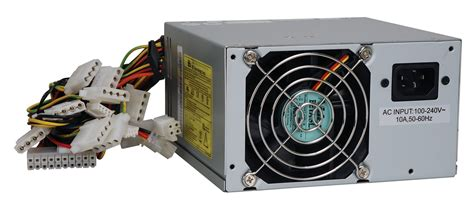
\includegraphics[width=\mythirdmaxsizeimageinsidetable]{chapter5/tablas comparativas/fuente de alimentacion 1.png} \\ 
				%\begin{myflushcenter}
				%	{\footnotesize Nombre imagen}
				%\end{myflushcenter}
			\end{minipage}
			&		  
			\begin{minipage}{\mythirdmaxsizeofcontenttable}
				\centering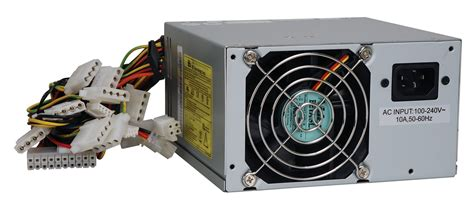
\includegraphics[width=\mythirdmaxsizeimageinsidetable]{chapter5/tablas comparativas/fuente de alimentacion 2.png} \\ 
				%\begin{myflushcenter}
				%	{\footnotesize Nombre imagen}
				%\end{myflushcenter}
			\end{minipage}
			&  
			\begin{minipage}{\mythirdmaxsizeofcontenttable}
				\centering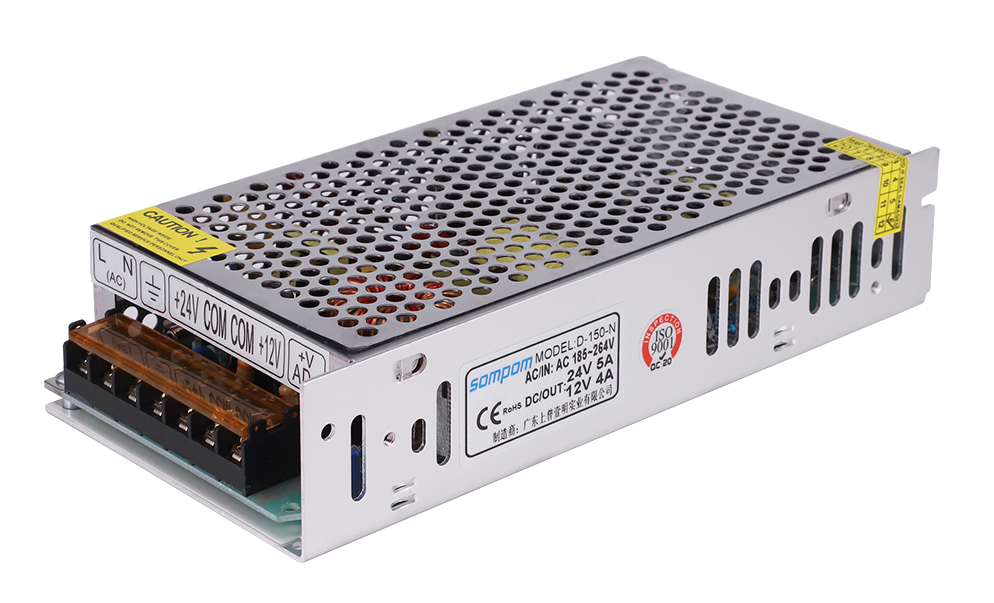
\includegraphics[width=\mythirdmaxsizeimageinsidetable]{chapter5/tablas comparativas/fuente de alimentacion 3.png} \\ 
				%\begin{myflushcenter}
				%	{\footnotesize Nombre imagen}
				%\end{myflushcenter}
			\end{minipage}\\ \hline
			\multicolumn{1}{|l|}{
				\begin{minipage}{\myforthmaxsizeofcontenttable}	
					\textbf{Fabricante}
				\end{minipage}
			} & - & 12SAF4 & AFAS222 & ASFASF \\ \hline
			\multicolumn{1}{|l|}{
				\begin{minipage}{\myforthmaxsizeofcontenttable}	
					\textbf{ABC}
				\end{minipage}
			} & 
			\begin{minipage}{\mythirdmaxsizeofcontenttable}\begin{myflushcenter}
					- 
			\end{myflushcenter}\end{minipage} & 
			\begin{minipage}{\mythirdmaxsizeofcontenttable}\begin{myflushcenter}
					1
			\end{myflushcenter}\end{minipage} &
			\begin{minipage}{\mythirdmaxsizeofcontenttable}\begin{myflushcenter}
					2 
			\end{myflushcenter}\end{minipage}&
			\begin{minipage}{\mythirdmaxsizeofcontenttable}\begin{myflushcenter}
					3 
			\end{myflushcenter}\end{minipage} \\ \hline
		\end{tabular}
		\begin{flushleft}	
			Fuente: Imágenes de dominio público y elaboración propia. Hoja de datos técnico (\textit{Datasheet}) en el Anexo.\\
			Tasa de cambio de USD a PEN: S/ 3.59.
		\end{flushleft}
	\end{mytable}
\end{savenotes}

\textcolor{blue}{[BORRADOR] Explicar la selección [/BORRADOR]}


%% NUEVO SUBSECCION X.X.X.X
\subsubsection{Selección de reguladores de voltaje de conmutación}

Los reguladores de voltaje de conmutación permiten dividir la tensión eléctrica continua de manera más eficiente comparado con otros métodos. En las Tablas \ref{tab:tabla comparativa de reguladores de voltaje de conmutacion1}, \ref{tab:tabla comparativa de reguladores de voltaje de conmutacion2} y \ref{tab:tabla comparativa de reguladores de voltaje de conmutacion3} se muestras los requerimientos mínimos para cada regulador dependiendo del voltaje de entrada y salida. La comparación de entre tres modelos permite una selección básica del componente óptimo.


%%%%%%%%%%%%%%%%%%%%%%%%%%%%%%%%%%%%%%%%%%%%%%%%%%%%%%%%%%%%%
%%% 11111111111111111111111111111111111111111111111111111 %%%
%%%%%%%%%%%%%%%%%%%%%%%%%%%%%%%%%%%%%%%%%%%%%%%%%%%%%%%%%%%%%

\begin{savenotes}
	\begin{mytable}[H]
		\centering
		\caption{Tabla comparativa de reguladores de voltaje de conmutación de X DC a Y DC.}
		\label{tab:tabla comparativa de reguladores de voltaje de conmutacion1}
		\begin{tabular}{l|c|c|c|c|}
			\cline{2-5}
			\multicolumn{1}{c|}{\textbf{}}            & \textbf{\begin{tabular}[c]{@{}c@{}}Requisitos\\ mínimos\end{tabular}} & 
			\multicolumn{1}{|l|}{				
				\begin{minipage}{\mythirdmaxsizeofcontenttable}
					\begin{myflushcenter}
						\textbf{T1}
					\end{myflushcenter}
				\end{minipage}
			}&
			\multicolumn{1}{|l|}{				
				\begin{minipage}{\mythirdmaxsizeofcontenttable}	
					\begin{myflushcenter}
						\textbf{T2}
					\end{myflushcenter}
				\end{minipage}
			}&
			\multicolumn{1}{|l|}{				
				\begin{minipage}{\mythirdmaxsizeofcontenttable}	
					\begin{myflushcenter}
						\textbf{T3}
					\end{myflushcenter}
				\end{minipage}
			}  \\ \hline
			\multicolumn{1}{|l|}{\textbf{Figura}} & - 
			&		  
			\begin{minipage}{\mythirdmaxsizeofcontenttable}
				\centering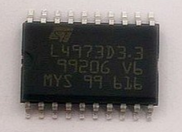
\includegraphics[width=\mythirdmaxsizeimageinsidetable]{chapter5/tablas comparativas/regulador de voltaje de conmutacion 1-1.png} \\ 
				%\begin{myflushcenter}
				%	{\footnotesize Nombre imagen}
				%\end{myflushcenter}
			\end{minipage}
			&		  
			\begin{minipage}{\mythirdmaxsizeofcontenttable}
				\centering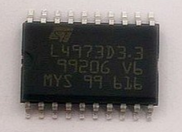
\includegraphics[width=\mythirdmaxsizeimageinsidetable]{chapter5/tablas comparativas/regulador de voltaje de conmutacion 1-2.png} \\ 
				%\begin{myflushcenter}
				%	{\footnotesize Nombre imagen}
				%\end{myflushcenter}
			\end{minipage}
			&  
			\begin{minipage}{\mythirdmaxsizeofcontenttable}
				\centering\includegraphics[width=\mythirdmaxsizeimageinsidetable]{chapter5/tablas comparativas/regulador de voltaje de conmutacion 1-3.png} \\ 
				%\begin{myflushcenter}
				%	{\footnotesize Nombre imagen}
				%\end{myflushcenter}
			\end{minipage}\\ \hline
			\multicolumn{1}{|l|}{
				\begin{minipage}{\myforthmaxsizeofcontenttable}	
					\textbf{Fabricante}
				\end{minipage}
			} & - & 12SAF4 & AFAS222 & ASFASF \\ \hline
			\multicolumn{1}{|l|}{
				\begin{minipage}{\myforthmaxsizeofcontenttable}	
					\textbf{ABC}
				\end{minipage}
			} & 
			\begin{minipage}{\mythirdmaxsizeofcontenttable}\begin{myflushcenter}
					- 
			\end{myflushcenter}\end{minipage} & 
			\begin{minipage}{\mythirdmaxsizeofcontenttable}\begin{myflushcenter}
					1
			\end{myflushcenter}\end{minipage} &
			\begin{minipage}{\mythirdmaxsizeofcontenttable}\begin{myflushcenter}
					2 
			\end{myflushcenter}\end{minipage}&
			\begin{minipage}{\mythirdmaxsizeofcontenttable}\begin{myflushcenter}
					3 
			\end{myflushcenter}\end{minipage} \\ \hline
		\end{tabular}
		\begin{flushleft}	
			Fuente: Imágenes de dominio público y elaboración propia. Hoja de datos técnico (\textit{Datasheet}) en el Anexo.\\
			Tasa de cambio de USD a PEN: S/ 3.59.
		\end{flushleft}
	\end{mytable}
\end{savenotes}

\textcolor{blue}{[BORRADOR] Explicar la selección [/BORRADOR]}

%%%%%%%%%%%%%%%%%%%%%%%%%%%%%%%%%%%%%%%%%%%%%%%%%%%%%%%%%%%%%
%%% 22222222222222222222222222222222222222222222222222222 %%%
%%%%%%%%%%%%%%%%%%%%%%%%%%%%%%%%%%%%%%%%%%%%%%%%%%%%%%%%%%%%%

\begin{savenotes}
	\begin{mytable}[H]
		\centering
		\caption{Tabla comparativa de reguladores de voltaje de conmutación de X DC a Y DC.}
		\label{tab:tabla comparativa de reguladores de voltaje de conmutacion2}
		\begin{tabular}{l|c|c|c|c|}
			\cline{2-5}
			\multicolumn{1}{c|}{\textbf{}}            & \textbf{\begin{tabular}[c]{@{}c@{}}Requisitos\\ mínimos\end{tabular}} & 
			\multicolumn{1}{|l|}{				
				\begin{minipage}{\mythirdmaxsizeofcontenttable}
					\begin{myflushcenter}
						\textbf{T1}
					\end{myflushcenter}
				\end{minipage}
			}&
			\multicolumn{1}{|l|}{				
				\begin{minipage}{\mythirdmaxsizeofcontenttable}	
					\begin{myflushcenter}
						\textbf{T2}
					\end{myflushcenter}
				\end{minipage}
			}&
			\multicolumn{1}{|l|}{				
				\begin{minipage}{\mythirdmaxsizeofcontenttable}	
					\begin{myflushcenter}
						\textbf{T3}
					\end{myflushcenter}
				\end{minipage}
			}  \\ \hline
			\multicolumn{1}{|l|}{\textbf{Figura}} & - 
			&		  
			\begin{minipage}{\mythirdmaxsizeofcontenttable}
				\centering\includegraphics[width=\mythirdmaxsizeimageinsidetable]{chapter5/tablas comparativas/regulador de voltaje de conmutacion 2-1.png} \\ 
				%\begin{myflushcenter}
				%	{\footnotesize Nombre imagen}
				%\end{myflushcenter}
			\end{minipage}
			&		  
			\begin{minipage}{\mythirdmaxsizeofcontenttable}
				\centering\includegraphics[width=\mythirdmaxsizeimageinsidetable]{chapter5/tablas comparativas/regulador de voltaje de conmutacion 2-2.png} \\ 
				%\begin{myflushcenter}
				%	{\footnotesize Nombre imagen}
				%\end{myflushcenter}
			\end{minipage}
			&  
			\begin{minipage}{\mythirdmaxsizeofcontenttable}
				\centering\includegraphics[width=\mythirdmaxsizeimageinsidetable]{chapter5/tablas comparativas/regulador de voltaje de conmutacion 2-3.png} \\ 
				%\begin{myflushcenter}
				%	{\footnotesize Nombre imagen}
				%\end{myflushcenter}
			\end{minipage}\\ \hline
			\multicolumn{1}{|l|}{
				\begin{minipage}{\myforthmaxsizeofcontenttable}	
					\textbf{Fabricante}
				\end{minipage}
			} & - & 12SAF4 & AFAS222 & ASFASF \\ \hline
			\multicolumn{1}{|l|}{
				\begin{minipage}{\myforthmaxsizeofcontenttable}	
					\textbf{ABC}
				\end{minipage}
			} & 
			\begin{minipage}{\mythirdmaxsizeofcontenttable}\begin{myflushcenter}
					- 
			\end{myflushcenter}\end{minipage} & 
			\begin{minipage}{\mythirdmaxsizeofcontenttable}\begin{myflushcenter}
					1
			\end{myflushcenter}\end{minipage} &
			\begin{minipage}{\mythirdmaxsizeofcontenttable}\begin{myflushcenter}
					2 
			\end{myflushcenter}\end{minipage}&
			\begin{minipage}{\mythirdmaxsizeofcontenttable}\begin{myflushcenter}
					3 
			\end{myflushcenter}\end{minipage} \\ \hline
		\end{tabular}
		\begin{flushleft}	
			Fuente: Imágenes de dominio público y elaboración propia. Hoja de datos técnico (\textit{Datasheet}) en el Anexo.\\
			Tasa de cambio de USD a PEN: S/ 3.59.
		\end{flushleft}
	\end{mytable}
\end{savenotes}

\textcolor{blue}{[BORRADOR] Explicar la selección [/BORRADOR]}

%%%%%%%%%%%%%%%%%%%%%%%%%%%%%%%%%%%%%%%%%%%%%%%%%%%%%%%%%%%%%
%%% 33333333333333333333333333333333333333333333333333333 %%%
%%%%%%%%%%%%%%%%%%%%%%%%%%%%%%%%%%%%%%%%%%%%%%%%%%%%%%%%%%%%%

\begin{savenotes}
	\begin{mytable}[H]
		\centering
		\caption{Tabla comparativa de reguladores de voltaje de conmutación de X DC a Y DC.}
		\label{tab:tabla comparativa de reguladores de voltaje de conmutacion3}
		\begin{tabular}{l|c|c|c|c|}
			\cline{2-5}
			\multicolumn{1}{c|}{\textbf{}}            & \textbf{\begin{tabular}[c]{@{}c@{}}Requisitos\\ mínimos\end{tabular}} & 
			\multicolumn{1}{|l|}{				
				\begin{minipage}{\mythirdmaxsizeofcontenttable}
					\begin{myflushcenter}
						\textbf{T1}
					\end{myflushcenter}
				\end{minipage}
			}&
			\multicolumn{1}{|l|}{				
				\begin{minipage}{\mythirdmaxsizeofcontenttable}	
					\begin{myflushcenter}
						\textbf{T2}
					\end{myflushcenter}
				\end{minipage}
			}&
			\multicolumn{1}{|l|}{				
				\begin{minipage}{\mythirdmaxsizeofcontenttable}	
					\begin{myflushcenter}
						\textbf{T3}
					\end{myflushcenter}
				\end{minipage}
			}  \\ \hline
			\multicolumn{1}{|l|}{\textbf{Figura}} & - 
			&		  
			\begin{minipage}{\mythirdmaxsizeofcontenttable}
				\centering\includegraphics[width=\mythirdmaxsizeimageinsidetable]{chapter5/tablas comparativas/regulador de voltaje de conmutacion 3-1.png} \\ 
				%\begin{myflushcenter}
				%	{\footnotesize Nombre imagen}
				%\end{myflushcenter}
			\end{minipage}
			&		  
			\begin{minipage}{\mythirdmaxsizeofcontenttable}
				\centering\includegraphics[width=\mythirdmaxsizeimageinsidetable]{chapter5/tablas comparativas/regulador de voltaje de conmutacion 3-2.png} \\ 
				%\begin{myflushcenter}
				%	{\footnotesize Nombre imagen}
				%\end{myflushcenter}
			\end{minipage}
			&  
			\begin{minipage}{\mythirdmaxsizeofcontenttable}
				\centering\includegraphics[width=\mythirdmaxsizeimageinsidetable]{chapter5/tablas comparativas/regulador de voltaje de conmutacion 3-3.png} \\ 
				%\begin{myflushcenter}
				%	{\footnotesize Nombre imagen}
				%\end{myflushcenter}
			\end{minipage}\\ \hline
			\multicolumn{1}{|l|}{
				\begin{minipage}{\myforthmaxsizeofcontenttable}	
					\textbf{Fabricante}
				\end{minipage}
			} & - & 12SAF4 & AFAS222 & ASFASF \\ \hline
			\multicolumn{1}{|l|}{
				\begin{minipage}{\myforthmaxsizeofcontenttable}	
					\textbf{ABC}
				\end{minipage}
			} & 
			\begin{minipage}{\mythirdmaxsizeofcontenttable}\begin{myflushcenter}
					- 
			\end{myflushcenter}\end{minipage} & 
			\begin{minipage}{\mythirdmaxsizeofcontenttable}\begin{myflushcenter}
					1
			\end{myflushcenter}\end{minipage} &
			\begin{minipage}{\mythirdmaxsizeofcontenttable}\begin{myflushcenter}
					2 
			\end{myflushcenter}\end{minipage}&
			\begin{minipage}{\mythirdmaxsizeofcontenttable}\begin{myflushcenter}
					3 
			\end{myflushcenter}\end{minipage} \\ \hline
		\end{tabular}
		\begin{flushleft}	
			Fuente: Imágenes de dominio público y elaboración propia. Hoja de datos técnico (\textit{Datasheet}) en el Anexo.\\
			Tasa de cambio de USD a PEN: S/ 3.59.
		\end{flushleft}
	\end{mytable}
\end{savenotes}

\textcolor{blue}{[BORRADOR] Explicar la selección [/BORRADOR]}

%% NUEVO SUBSECCION X.X.X.X
\subsubsection{Diagrama esquemático} 

\textcolor{blue}{[BORRADOR] Explicar el diagrama esquemático [/BORRADOR]}

\begin{myfigure}[H]
	\centering
	\includegraphics[width=1\textwidth]{chapter5/diagrama esquematico.pdf}
	\caption{Diagrama esquemático del sistema}
	\begin{myflushleftportland}
		Fuente: Elaboración propia. Hoja de datos técnico (\textit{Datasheet}) en el Anexo.
	\end{myflushleftportland}
	\label{fig:diagrama esquematico}
\end{myfigure}

%% NUEVO SUBSECCION X.X.X.X
%\subsubsection{Diagrama eléctrico} 


%% NUEVA SECCIÓN X.X.X
\subsection{Subsistema de control e interacción con el usuario}
\label{ssec:subsistema de control e interaccion con el usuario}

El presente subsistema tiene como fin monitorear y controlar los sensores y actuadores, establecer comunicación con los dispositivos de interacción con el usuario tal como un celular o una computadora portátil. Consecuentemente, en las siguientes subsecciones se detalla: la selección de componentes, el cálculo de consumo de energía del sistema, diagrama de flujo de los procesadores de datos y finalmente el diseño frontend de la aplicación móvil.


%% NUEVO SUBSECCION X.X.X.X
\subsubsection{Selección de microprocesador}
\label{sssec:seleccion de microprocesador}

El microprocesador se encarga de recibir los datos que le envía el módulo de procesamiento de imágenes tanto de la cámara estéreo como de la cámara simple. Si bien el procesamiento de imágenes se realiza en los módulos mencionados\footnote{Las cámaras cuentan con procesadores incorporados especializados en imágenes.}, el control de abrir/cerrar compuertas mediante el accionamiento de los motores a paso, control PID de las electroválvulas y conexión con el subsistema de interacción con el usuario se realizan en el microprocesador. Las funciones anteriormente mencionadas se traducen en una serie de requisitos en los tipos y números de pines que se muestran de manera técnica en la Tabla \ref{tab:pines necesarios en el microprocesador}.

%%%%%%%%%%%%%%%%%%%%%%%%%%%%%%%%%%%%%%%%%%%%%%%%%%%%%%
%- Necesitamos: 80 fps \\
%- Tamaño máximo: 15 cm \\
%- Tamaño mínimo: 20 cm \\
%- Velocidad estándar: 2 - 3 L/s (Longitud/segundos) \\
%- Velocidad máxima: 3 - 4 L/s (Longitud/segundos) \\

%En la Sección \ref{sssec:seleccion de algoritmo de clasificacion y conteo} se analiza los posibles algoritmos que pueden ser aplicados para la detección de truchas mediante visión por computadora.
%%%%%%%%%%%%%%%%%%%%%%%%%%%%%%%%%%%%%%%%%%%%%%%%%%%%%%

\begin{mytable}[H]
	\centering
	\caption{Pines necesarios en el microprocesador.}
	\label{tab:pines necesarios en el microprocesador}
	\begin{tabular}{|c|c|c|c|}
		\hline
		\textbf{Descripción} & \textbf{Nro. de pines} & \textbf{Tipo de comunicación} & \textbf{Entrada/Salida} \\ \hline
		Control LED Iluminación 1 & 1 & GPIO                  & Salida        \\ \hline
		Control LED Iluminación 2 & 1 & GPIO                  & Salida        \\ \hline
		Indicador: Bocina         & 1 & GPIO                  & Salida        \\ \hline
		Indicador: LED            & 1 & GPIO                  & Salida        \\ \hline
		Control Electroválvula 1  & 1 & GPIO                  & Salida        \\ \hline
		Control Electroválvula 2  & 1 & GPIO                  & Salida        \\ \hline
		Control Electroválvula 3  & 1 & GPIO                  & Salida        \\ \hline
		Control Electroválvula 4  & 1 & GPIO                  & Salida        \\ \hline
		Cámara estéreo            & 1 & \textgreater{}USB 3.0 & Bidireccional \\ \hline
		Cámara simple             & 1 & \textgreater{}USB 3.0 & Bidireccional \\ \hline
		Control Bombas de agua    & 3 & I2C                   & Bidireccional \\ \hline
		Control Motor a pasos     & 3 & GPIO                  & Salida        \\ \hline
	\end{tabular}
	\begin{flushleft}	
	Fuente: Elaboración propia.
	\end{flushleft}
\end{mytable}

En la Tabla \ref{tab:tabla comparativa de microprocesadores} se muestran los requerimientos mínimos y tres alternativas para escoger el microprocesador óptimo. Dichos requerimientos mínimos contemplan características técnicas: consumo de energía, cantidad de pines, velocidad de procesamiento, tipos de comunicación, etc.

\begin{savenotes}
	\begin{mytable}[H]
		\centering
		\caption{Tabla comparativa de microprocesadores.}
		\label{tab:tabla comparativa de microprocesadores}
		\begin{tabular}{l|c|c|c|c|}
			\cline{2-5}
			\multicolumn{1}{c|}{\textbf{}} & \textbf{\begin{tabular}[c]{@{}c@{}}Requisitos\\ mínimos\end{tabular}} & 
			\multicolumn{1}{|l|}{				
				\begin{minipage}{\mythirdmaxsizeofcontenttable}
					\begin{myflushcenter}
						\textbf{Raspberry Pi 4 B}
					\end{myflushcenter}
				\end{minipage}
			}&
			\multicolumn{1}{|l|}{				
				\begin{minipage}{\mythirdmaxsizeofcontenttable}	
					\begin{myflushcenter}
						\textbf{ASUS Tinker Board S}
					\end{myflushcenter}
				\end{minipage}
			}&
			\multicolumn{1}{|l|}{				
				\begin{minipage}{\mythirdmaxsizeofcontenttable}	
					\begin{myflushcenter}
						\textbf{Helios64}
					\end{myflushcenter}
				\end{minipage}
			}  \\ \hline
			\multicolumn{1}{|l|}{\textbf{Figura}} & - 
			&		  
			\begin{minipage}{\mythirdmaxsizeofcontenttable}
				\centering\includegraphics[width=\mythirdmaxsizeimageinsidetable]{chapter5/tablas comparativas/microprocesador 1.png} \\ 
				%\begin{myflushcenter}
				%	{\footnotesize Nombre imagen}
				%\end{myflushcenter}
			\end{minipage}
			&		  
			\begin{minipage}{\mythirdmaxsizeofcontenttable}
				\centering\includegraphics[width=\mythirdmaxsizeimageinsidetable]{chapter5/tablas comparativas/microprocesador 2.png} \\ 
				%\begin{myflushcenter}
				%	{\footnotesize Nombre imagen}
				%\end{myflushcenter}
			\end{minipage}
			&  
			\begin{minipage}{\mythirdmaxsizeofcontenttable}
				\centering\includegraphics[width=\mythirdmaxsizeimageinsidetable]{chapter5/tablas comparativas/microprocesador 3.png} \\ 
				%\begin{myflushcenter}
				%	{\footnotesize Nombre imagen}
				%\end{myflushcenter}
			\end{minipage}\\ \hline
			\multicolumn{1}{|l|}{
				\begin{minipage}{\myforthmaxsizeofcontenttable}	
					\textbf{Fabricante}
				\end{minipage}
			} & - & Raspberry & ASUS & Kobol \\ \hline
			\multicolumn{1}{|l|}{
				\begin{minipage}{\myforthmaxsizeofcontenttable}	
					\textbf{CPU}
				\end{minipage}
			} & 
			\begin{minipage}{\mythirdmaxsizeofcontenttable}\begin{myflushcenter}
					0.5 Ghz 
			\end{myflushcenter}\end{minipage} & 
			\begin{minipage}{\mythirdmaxsizeofcontenttable}\begin{myflushcenter}
					ARM Cortex A72@ 1.5 GHz
			\end{myflushcenter}\end{minipage} &
			\begin{minipage}{\mythirdmaxsizeofcontenttable}\begin{myflushcenter}
					Quad-Core RK3288
			\end{myflushcenter}\end{minipage}&
			\begin{minipage}{\mythirdmaxsizeofcontenttable}\begin{myflushcenter}
					ARM 64-bit Hexacore 
			\end{myflushcenter}\end{minipage} \\ \hline		
			\multicolumn{1}{|l|}{
				\begin{minipage}{\myforthmaxsizeofcontenttable}	
					\textbf{Pines GPIO}
				\end{minipage}
			} & 8 & 40 & 28 & 20 \\ \hline		
			\multicolumn{1}{|l|}{
				\begin{minipage}{\myforthmaxsizeofcontenttable}	
					\textbf{Conexiones USB}
				\end{minipage}
			} & 2xUSB 3.0 & 
			\begin{minipage}{\mythirdmaxsizeofcontenttable}\begin{myflushcenter}
					2xUSB2.0 y 2xUSB3.0
			\end{myflushcenter}\end{minipage}
		 	& 2xUSB3.0 & 3xUSB3.0 \\ \hline	
			\multicolumn{1}{|l|}{
				\begin{minipage}{\myforthmaxsizeofcontenttable}	
					\textbf{Conexión a Internet}
				\end{minipage}
			} & WiFi 2.4Ghz & 
			\begin{minipage}{\mythirdmaxsizeofcontenttable}\begin{myflushcenter}
				Ethernet y WiFi 2.4Ghz- 5Ghz
			\end{myflushcenter}\end{minipage}
			 & WiFi 2.4Ghz & 
			 \begin{minipage}{\mythirdmaxsizeofcontenttable}\begin{myflushcenter}
			 		Ethernet y WiFi 2.4Ghz- 5Ghz
			 \end{myflushcenter}\end{minipage} \\ \hline		
			\multicolumn{1}{|l|}{
				\begin{minipage}{\myforthmaxsizeofcontenttable}	
					\textbf{Voltaje de alimentación ($V$)}
				\end{minipage}
			} & 5 & 5 & 5 & 12 \\ \hline			
			\multicolumn{1}{|l|}{
				\begin{minipage}{\myforthmaxsizeofcontenttable}	
					\textbf{Consumo de corriente\footnote{En uso típico.} ($A$)}
				\end{minipage}
			} & - & 3 & 3 & 3 \\ \hline
			\multicolumn{1}{|l|}{
				\begin{minipage}{\myforthmaxsizeofcontenttable}	
					\textbf{Procesador gráfico}
				\end{minipage}
			} & - & VideoCore VI & 		
			\begin{minipage}{\mythirdmaxsizeofcontenttable}\begin{myflushcenter}
				ARM® Mali™-T764 GPU
			\end{myflushcenter}\end{minipage}
			 &  		
			\begin{minipage}{\mythirdmaxsizeofcontenttable}\begin{myflushcenter}
				Mali-T860MP4
			\end{myflushcenter}\end{minipage} \\ \hline		
			\multicolumn{1}{|l|}{
				\begin{minipage}{\myforthmaxsizeofcontenttable}	
					\textbf{Cantidad de pines PWM}
				\end{minipage}
			} & - & 4 & 4 & 2 \\ \hline		
			\multicolumn{1}{|l|}{
				\begin{minipage}{\myforthmaxsizeofcontenttable}	
					\textbf{Cantidad de pines I2C}
				\end{minipage}
			} & 2 & 4 & 4 & 2 \\ \hline		
			\multicolumn{1}{|l|}{
				\begin{minipage}{\myforthmaxsizeofcontenttable}	
					\textbf{RAM (GB)}
				\end{minipage}
			} & - & 4 & 2 & 4 \\ \hline
			\multicolumn{1}{|l|}{
				\begin{minipage}{\myforthmaxsizeofcontenttable}	
					\textbf{Precio ($S/$)}
				\end{minipage}
			} & - & 197.45 & 327.19 & 678.51 \\ \hline		
		\end{tabular}
		\begin{flushleft}	
			Fuente: Imágenes de dominio público y elaboración propia. Hoja de datos técnico (\textit{Datasheet}) en el Anexo.\\
			Tasa de cambio de USD a PEN: S/ 3.59.
		\end{flushleft}
	\end{mytable}
\end{savenotes}

\textcolor{blue}{[BORRADOR] Seleccionar y explicar selección... [/BORRADOR]}

%% NUEVO SUBSECCION X.X.X.X
\subsubsection{Selección de indicadores}

Los indicadores ya sean visuales o sonoros son parte fundamental de una máquina y se usan los dos tipos de indicadores para redundar el sistema de alertas de la CCT\footnote{Máquina Contadora y Clasificadora de Truchas.}. En el caso de la CCT el sistema debe indicar al operario diversos estados o funciones: al detectar una trucha, al contar una trucha, al encender y al apagar.

\begin{itemize}
	\item \textbf{Indicador visual:} Los indicadores visuales indican al usuario diversos estados de la máquina: prendido, procesando, apagado y error general. Por lo que el indicador visual, además de ser visible bajo la luz del día, brinda una gama de colores superior a 4 fácilmente diferenciables. Los indicadores visuales LED son ideales para esta situación. En la Tabla \ref{tab:tabla comparativa de indicadores visuales} se comparan tres dispositivos que cumplen con los requerimientos mínimos.	
	
	\begin{savenotes}
		\begin{mytable}[H]
			\centering
			\caption{Tabla comparativa de indicadores visuales.}
			\label{tab:tabla comparativa de indicadores visuales}
			\begin{tabular}{l|c|c|c|c|}
				\cline{2-5}
				\multicolumn{1}{c|}{\textbf{}} & \textbf{\begin{tabular}[c]{@{}c@{}}Requisitos\\ mínimos\end{tabular}} & 
				\multicolumn{1}{|l|}{				
					\begin{minipage}{\mythirdmaxsizeofcontenttable}
						\begin{myflushcenter}
							\textbf{111111}
						\end{myflushcenter}
					\end{minipage}
				}&
				\multicolumn{1}{|l|}{				
					\begin{minipage}{\mythirdmaxsizeofcontenttable}	
						\begin{myflushcenter}
							\textbf{222222}
						\end{myflushcenter}
					\end{minipage}
				}&
				\multicolumn{1}{|l|}{				
					\begin{minipage}{\mythirdmaxsizeofcontenttable}	
						\begin{myflushcenter}
							\textbf{333333}
						\end{myflushcenter}
					\end{minipage}
				}  \\ \hline
				\multicolumn{1}{|l|}{\textbf{Figura}} & - 
				&		  
				\begin{minipage}{\mythirdmaxsizeofcontenttable}
					\centering\includegraphics[width=\mythirdmaxsizeimageinsidetable]{chapter5/tablas comparativas/indicador visual 1.png} \\ 
					%\begin{myflushcenter}
					%	{\footnotesize Nombre imagen}
					%\end{myflushcenter}
				\end{minipage}
				&		  
				\begin{minipage}{\mythirdmaxsizeofcontenttable}
					\centering\includegraphics[width=\mythirdmaxsizeimageinsidetable]{chapter5/tablas comparativas/indicador visual 2.png} \\ 
					%\begin{myflushcenter}
					%	{\footnotesize Nombre imagen}
					%\end{myflushcenter}
				\end{minipage}
				&  
				\begin{minipage}{\mythirdmaxsizeofcontenttable}
					\centering\includegraphics[width=\mythirdmaxsizeimageinsidetable]{chapter5/tablas comparativas/indicador visual 3.png} \\ 
					%\begin{myflushcenter}
					%	{\footnotesize Nombre imagen}
					%\end{myflushcenter}
				\end{minipage}\\ \hline
				\multicolumn{1}{|l|}{
					\begin{minipage}{\myforthmaxsizeofcontenttable}	
						\textbf{Fabricante}
					\end{minipage}
				} & - & AAAA & AAAA & AAAAAA \\ \hline
				\multicolumn{1}{|l|}{
					\begin{minipage}{\myforthmaxsizeofcontenttable}	
						\textbf{Tipo de obturador}
					\end{minipage}
				} & 
				\begin{minipage}{\mythirdmaxsizeofcontenttable}\begin{myflushcenter}
						ASFASFSAF 
				\end{myflushcenter}\end{minipage} & 
				\begin{minipage}{\mythirdmaxsizeofcontenttable}\begin{myflushcenter}
						WERWRWER 
				\end{myflushcenter}\end{minipage} &
				\begin{minipage}{\mythirdmaxsizeofcontenttable}\begin{myflushcenter}
						ASFASF
				\end{myflushcenter}\end{minipage}&
				\begin{minipage}{\mythirdmaxsizeofcontenttable}\begin{myflushcenter}
						AAAAA 
				\end{myflushcenter}\end{minipage} \\ \hline
			\end{tabular}
			\begin{flushleft}	
				Fuente: Imágenes de dominio público y elaboración propia. Hoja de datos técnico (\textit{Datasheet}) en el Anexo.\\
				Tasa de cambio de USD a PEN: S/ 3.59.
			\end{flushleft}
		\end{mytable}
	\end{savenotes}

	\textcolor{blue}{[BORRADOR] Seleccionar y explicar [/BORRADOR]}	
		
	\item \textbf{Indicador sonoro:} Similar a un indicador visual, una bocina indica al operario el estado de la máquina. Sin embargo, los indicadores sonoros son perfectos para alertar al operario de algún mal funcionamiento de la máquina. En la Tabla \ref{tab:tabla comparativa de bocinas} se compara características técnicas entre algunas bocinas candidatas para el sistema.

	\begin{mytable}[H]
		\centering
		\caption{Tabla comparativa de bocinas}
		\label{tab:tabla comparativa de bocinas}
		\begin{tabular}{l|c|c|c|c|}
			\cline{2-5}
			\multicolumn{1}{c|}{\textbf{}}                         & \textbf{\begin{tabular}[c]{@{}c@{}}Requisitos\\ mínimos\end{tabular}} & \textbf{SE-B40} & \textbf{KH} & \textbf{TS-G1010F} \\ \hline
			\multicolumn{1}{|l|}{\textbf{Figura}}&
			-
			&
			\begin{minipage}{\mythirdmaxsizeofcontenttable}
				\centering\includegraphics[width=\mythirdmaxsizeimageinsidetable]{chapter5/tablas comparativas/bocina 1.png} \\ 
				%\begin{myflushcenter}
				%	{\footnotesize Nombre imagen}
				%\end{myflushcenter}
			\end{minipage}  
			&
			\begin{minipage}{\mythirdmaxsizeofcontenttable}
				\centering\includegraphics[width=\mythirdmaxsizeimageinsidetable]{chapter5/tablas comparativas/bocina 2.png} \\ 
				%\begin{myflushcenter}
				%	{\footnotesize Nombre imagen}
				%\end{myflushcenter}
			\end{minipage}
			&  
			\begin{minipage}{\mythirdmaxsizeofcontenttable}
				\centering\includegraphics[width=\mythirdmaxsizeimageinsidetable]{chapter5/tablas comparativas/bocina 3.png} \\ 
				%\begin{myflushcenter}
				%	{\footnotesize Nombre imagen}
				%\end{myflushcenter}
			\end{minipage}  \\ \hline
			\multicolumn{1}{|l|}{\textbf{Fabricante}}              & -                                                                     &                 &             &                    \\ \hline
			\multicolumn{1}{|l|}{\textbf{Dimensión (cm.)}}         & -                                                                     &                 &             &                    \\ \hline
			\multicolumn{1}{|l|}{				
				\begin{minipage}{\myforthmaxsizeofcontenttable}	
					\textbf{Frecuencia de trabajo (Hz)}
				\end{minipage}
			}   & -                                                                     &                 &             &                    \\ \hline
			\multicolumn{1}{|l|}{
				\begin{minipage}{\myforthmaxsizeofcontenttable}	
					\textbf{Voltaje de alimentación (V)}
				\end{minipage}
			} & -                                                                     & 12 VDC          & 12 VDC      & 12 VDC             \\ \hline
			\multicolumn{1}{|l|}{\textbf{RMS (W)}}                 & -                                                                     & 80              & 25          & 30                 \\ \hline
			\multicolumn{1}{|l|}{\textbf{Precio (S/)}}             & -                                                                     & 105             & 105         & 79                 \\ \hline
			\multicolumn{1}{|l|}{\textbf{Disponibilidad}}          & Inmediata                                                             & A pedido        & A pedido    & A pedido           \\ \hline
		\end{tabular}
		\begin{flushleft}	
			Fuente: Imágenes de dominio público, %%%%%%%%%%%%%%%%%%%%%%%%%%%%%%%%%%%\cite{DiazVergara2019}
			 y elaboración propia.
		\end{flushleft}
	\end{mytable}

	\textcolor{blue}{[BORRADOR] Seleccionar y explicar [/BORRADOR]}
	
\end{itemize}

%% NUEVO SUBSECCION X.X.X.X
\subsubsection{Selección de interruptor de seguridad de apagado de emergencia}

La implementación de un interruptor de seguridad es muy importante en el diseño de máquinas ya que es el mecanismo físico por el cual podemos parar la máquina quitando el suministro eléctrico a todos los componentes. En la Tabla \ref{tab:tabla comparativa de interruptor de seguridad de apagado de emergencia} se compara características técnicas entre interruptor de seguridad candidatos para el sistema.

\begin{mytable}[H]
	\centering
	\caption{Tabla comparativa de interruptor de seguridad de apagado de emergencia.}
	\label{tab:tabla comparativa de interruptor de seguridad de apagado de emergencia}
	\begin{tabular}{l|c|c|c|c|}
		\cline{2-5}
		\multicolumn{1}{c|}{\textbf{}}                          & \textbf{\begin{tabular}[c]{@{}c@{}}Requisitos\\ mínimos\end{tabular}} & \textbf{1} & \textbf{2} & \textbf{3} \\ \hline
		\multicolumn{1}{|l|}{\textbf{Figura}}&
		-
		&
		\begin{minipage}{\mythirdmaxsizeofcontenttable}
			\centering\includegraphics[width=\mythirdmaxsizeimageinsidetable]{chapter5/tablas comparativas/interruptor de seguridad de apagado de emergencia 1.png} \\ 
			%\begin{myflushcenter}
			%	{\footnotesize Nombre imagen}
			%\end{myflushcenter}
		\end{minipage}  
		&
		\begin{minipage}{\mythirdmaxsizeofcontenttable}
			\centering\includegraphics[width=\mythirdmaxsizeimageinsidetable]{chapter5/tablas comparativas/interruptor de seguridad de apagado de emergencia 2.png} \\ 
			%\begin{myflushcenter}
			%	{\footnotesize Nombre imagen}
			%\end{myflushcenter}
		\end{minipage}
		&  
		\begin{minipage}{\mythirdmaxsizeofcontenttable}
			\centering\includegraphics[width=\mythirdmaxsizeimageinsidetable]{chapter5/tablas comparativas/interruptor de seguridad de apagado de emergencia 3.png} \\ 
			%\begin{myflushcenter}
			%	{\footnotesize Nombre imagen}
			%\end{myflushcenter}
		\end{minipage}  \\ \hline
		\multicolumn{1}{|l|}{\textbf{Fabricante}}               & -                                                                     & 9          & 10         & 11         \\ \hline
		\multicolumn{1}{|l|}{\textbf{Nivel de protección}}      & 12                                                                    & 13         & 14         & 15         \\ \hline
		\multicolumn{1}{|l|}{
			\begin{minipage}{\myforthmaxsizeofcontenttable}			
				\textbf{Máximo voltaje admisible (V)}
			\end{minipage}
		}
		&
		16
		& 17         & 18         & 19         \\ \hline
		\multicolumn{1}{|l|}{
			\begin{minipage}{\myforthmaxsizeofcontenttable}			
				\textbf{Diámetro del botón (mm.)}
			\end{minipage}
		} & 20                                                                    & 21         & 22         & 23         \\ \hline
		\multicolumn{1}{|l|}{\textbf{Precio (S/)}}              & 24                                                                    & 25         & 26         & 27         \\ \hline
		\multicolumn{1}{|l|}{\textbf{Disponibilidad}}           & 32                                                                    & 33         & 34         & 35         \\ \hline
	\end{tabular}
	\begin{flushleft}	
		Fuente: Imágenes de dominio público y elaboración propia.
	\end{flushleft}
\end{mytable}

\textcolor{blue}{[BORRADOR] Seleccionar y explicar [/BORRADOR]}


%% NUEVO SUBSECCION X.X.X.X
\subsubsection{Selección de interruptor de interruptor tipo hongo}

El encendido o apagado de la máquina es realizado por este interruptor, es decir, el control del suministro de energía del sistema depende de dicho dispositivo. En la Tabla \ref{tab:tabla comparativa de interruptor de interruptor tipo hongo} se compara características técnicas entre interruptores tipo hongo candidatos para el sistema.

\begin{mytable}[H]
\centering
\caption{Tabla comparativa de interruptor de interruptor tipo hongo.}
\label{tab:tabla comparativa de interruptor de interruptor tipo hongo}
\begin{tabular}{l|c|c|c|c|}
	\cline{2-5}
	\multicolumn{1}{c|}{\textbf{}}                          & \textbf{\begin{tabular}[c]{@{}c@{}}Requisitos\\ mínimos\end{tabular}} & \textbf{1} & \textbf{2} & \textbf{3} \\ \hline
	\multicolumn{1}{|l|}{\textbf{Figura}}&
	-
	&
	\begin{minipage}{\mythirdmaxsizeofcontenttable}
		\centering\includegraphics[width=\mythirdmaxsizeimageinsidetable]{chapter5/tablas comparativas/interruptor tipo hongo 1.png} \\ 
		%\begin{myflushcenter}
		%	{\footnotesize Nombre imagen}
		%\end{myflushcenter}
	\end{minipage}  
	&
	\begin{minipage}{\mythirdmaxsizeofcontenttable}
		\centering\includegraphics[width=\mythirdmaxsizeimageinsidetable]{chapter5/tablas comparativas/interruptor tipo hongo 2.png} \\ 
		%\begin{myflushcenter}
		%	{\footnotesize Nombre imagen}
		%\end{myflushcenter}
	\end{minipage}
	&  
	\begin{minipage}{\mythirdmaxsizeofcontenttable}
		\centering\includegraphics[width=\mythirdmaxsizeimageinsidetable]{chapter5/tablas comparativas/interruptor tipo hongo 3.png} \\ 
		%\begin{myflushcenter}
		%	{\footnotesize Nombre imagen}
		%\end{myflushcenter}
	\end{minipage}  \\ \hline
	\multicolumn{1}{|l|}{\textbf{Fabricante}}               & -                                                                     & 9          & 10         & 11         \\ \hline
	\multicolumn{1}{|l|}{\textbf{Nivel de protección}}      & 12                                                                    & 13         & 14         & 15         \\ \hline
	\multicolumn{1}{|l|}{
		\begin{minipage}{\myforthmaxsizeofcontenttable}			
			\textbf{Máximo voltaje admisible (V)}
		\end{minipage}
	} &
	16
	& 17         & 18         & 19         \\ \hline
	\multicolumn{1}{|l|}{
			\begin{minipage}{\myforthmaxsizeofcontenttable}			
				\textbf{Diámetro del botón (mm.)}
			\end{minipage}
	} & 20                                                                    & 21         & 22         & 23         \\ \hline
	\multicolumn{1}{|l|}{\textbf{Precio (S/)}}              & 24                                                                    & 25         & 26         & 27         \\ \hline
	\multicolumn{1}{|l|}{\textbf{Disponibilidad}}           & 32                                                                    & 33         & 34         & 35         \\ \hline
	\end{tabular}
	\begin{flushleft}	
		Fuente: Imágenes de dominio público y elaboración propia.
	\end{flushleft}
\end{mytable}

\textcolor{blue}{[BORRADOR] Seleccionar y explicar [/BORRADOR]}

%% NUEVO SUBSECCION X.X.X.X
\subsubsection{Cálculo del consumo de energía del sistema} 

El cálculo del consumo de energía del sistema es la suma de potencia requerida por cada componente. Dicha información se presenta en la Tabla \ref{fig:potencia requerida por componente}, además se muestra el modelo, la potencia máxima, voltaje de cada componente. Se considera, también, la cantidad de cada modelo de componente electrónico usado en el sistema.

% TIENE QUE SER TABLA
% TIENE QUE SER TABLA
% TIENE QUE SER TABLA
% TIENE QUE SER TABLA
% TIENE QUE SER TABLA
     
\begin{myfigure}[H]
	\centering
	\includegraphics[width=1\textwidth]{chapter5/potencia requerida por componente.png}
	\caption{Potencia requerida por componente}
	\begin{myflushleftportland}
		Fuente: Elaboración propia.
	\end{myflushleftportland}
	\label{fig:potencia requerida por componente}
\end{myfigure}


%% NUEVO SUBSECCION X.X.X.X
\subsubsection{Diagrama de flujo}

El diagrama de flujo principal, expuesto en la Figura \ref{fig:diagrama de flujo} describe los pasos necesarios para el control del sistema. \textcolor{blue}{[BORRADOR] Explicar diagrama de flujo [/BORRADOR]}

\begin{myfigure}[H]
	\centering
	\includegraphics[width=1\textwidth]{chapter5/diagrama de flujo.png}
	\caption{Diagrama de flujo principal}
	\begin{myflushleftportland}
		Fuente: Elaboración propia.
	\end{myflushleftportland}
	\label{fig:diagrama de flujo}
\end{myfigure}


%% NUEVO SUBSECCION X.X.X.X
\subsubsection{Diseño frontend de la aplicación móvil}

La aplicación móvil permitirá a un operario visualizar los estados de la máquina, así como tener un registro de la clasificación y conteo de truchas, es decir, extraer los datos luego de ser procesados por la máquina CCT de manera inalámbrica al terminar el proceso. Además, posterior a este trabajo, podría agregarse más características al aplicativo móvil. El framework de desarrollo del aplicativo, que no se desarrollará en el presente trabajo, escogido es Flutter por su paradigma multiplataforma, es decir, escribir un programa que se vea igual en los sistemas operativos Android y iOS \cite{Simone2020}. El diseño frontend escogido para el proyecto y su desarrollo sencillo 


\textcolor{blue}{[BORRADOR] 
	Bibliografía:\\
	Designing the obvious
	\cite{Joekman2010} \\
	Google Flutter Mobile Development Quick Start Guide
	\cite{PrajyotMainkar2019} \\
	Mobile Learning Design: Theories and Application
	\cite{Churchill2016} \\
	Mobile Design Pattern Gallery: UI Patterns for Mobile Applications
	\cite{Neil2012}
	[/BORRADOR]}



\begin{myfigure}[H]
	\centering
	\includegraphics[width=1\textwidth]{chapter5/aplicacion movil login.png}
	\caption{Aplicación móvil: inicio de sesión}
	\begin{myflushleftportland}
		Fuente: Elaboración propia.
	\end{myflushleftportland}
	\label{fig:aplicacion movil login}
\end{myfigure}


%% NUEVA SECCIÓN X.X.X
\subsection{Subsistema de flotación}
\label{ssec:subsistema de flotacion}

Luego de definir en las Secciones \ref{ssec:subsistema de recepcion y traslado de truchas}, \ref{ssec:subsistema de procesamiento de imágenes}, \ref{ssec:subsistema de suministro de energia}, y \ref{ssec:subsistema de control e interaccion con el usuario}, la selección de los dispositivos y su interacción el sistema permiten calcular las dimensiones de la máquina para analizar la flotabilidad y seleccionar flotadores adecuados. En las siguientes subsecciones se analizan los cálculos, selección y diseño del sistema de flotación.

%% NUEVO SUBSECCION X.X.X.X
\subsubsection{Cálculo de fuerzas necesarias para mantener a flote el sistema}

\textcolor{blue}{[BORRADOR] Explicar subsección e importancia [/BORRADOR]} 

\begin{myfigure}[H]
	\centering
	\includegraphics[width=1\textwidth]{chapter5/calculo de fuerzas necesarias para mantener a flote el sistema.png}
	\caption{Fuerzas necesarias para mantener a flote el sistema}
	\begin{myflushleftportland}
		Fuente: Elaboración propia.
	\end{myflushleftportland}
	\label{fig:calculo de fuerzas necesarias para mantener a flote el sistema}
\end{myfigure}

\textcolor{blue}{[BORRADOR] Ecuaciones y resultados [/BORRADOR]} 

%% NUEVO SUBSECCION X.X.X.X
\subsubsection{Selección de flotadores}

\textcolor{blue}{[BORRADOR] Introducción [/BORRADOR]} 

\begin{mytable}[H]
	\centering
	\caption{Tabla comparativa de flotadores.}
	\label{tab:tabla comparativa de flotadores}
	\begin{tabular}{l|c|c|c|c|}
		\cline{2-5}
		\multicolumn{1}{c|}{\textbf{}} & \textbf{\begin{tabular}[c]{@{}c@{}}Requisitos\\ mínimos\end{tabular}} &
		\begin{minipage}{\mythirdmaxsizeofcontenttable}\begin{myflushcenter}
			\textbf{1}
		\end{myflushcenter}\end{minipage} & 
		\begin{minipage}{\mythirdmaxsizeofcontenttable}\begin{myflushcenter}
			\textbf{2}
		\end{myflushcenter}\end{minipage} &
		\begin{minipage}{\mythirdmaxsizeofcontenttable}\begin{myflushcenter}
			\textbf{3}
		\end{myflushcenter}\end{minipage} \\ \hline
		\multicolumn{1}{|l|}{\textbf{Figura}}& - &
		\begin{minipage}{\mythirdmaxsizeofcontenttable}
			\centering\includegraphics[width=\mythirdmaxsizeimageinsidetable]{chapter5/tablas comparativas/flotador 1.png} \\ 
			%\begin{myflushcenter}
			%	{\footnotesize Nombre imagen}
			%\end{myflushcenter}
		\end{minipage}  
		&
		\begin{minipage}{\mythirdmaxsizeofcontenttable}
			\centering\includegraphics[width=\mythirdmaxsizeimageinsidetable]{chapter5/tablas comparativas/flotador 2.png} \\ 
			%\begin{myflushcenter}
			%	{\footnotesize Nombre imagen}
			%\end{myflushcenter}
		\end{minipage}
		&  
		\begin{minipage}{\mythirdmaxsizeofcontenttable}
			\centering\includegraphics[width=\mythirdmaxsizeimageinsidetable]{chapter5/tablas comparativas/flotador 3.png} \\ 
			%\begin{myflushcenter}
			%	{\footnotesize Nombre imagen}
			%\end{myflushcenter}
		\end{minipage}  \\ \hline
		\multicolumn{1}{|l|}{
			\begin{minipage}{\myforthmaxsizeofcontenttable}			
				\textbf{Concepto}
			\end{minipage}
		} & - & 9 & 10 & 11 \\ \hline
		\multicolumn{1}{|l|}{
			\begin{minipage}{\myforthmaxsizeofcontenttable}			
				\textbf{Concepto}
			\end{minipage}
		} & - & 9 & 10 & 11 \\ \hline
	
	\end{tabular}
	\begin{flushleft}	
		Fuente: Elaboración propia.
	\end{flushleft}
\end{mytable}

\textcolor{blue}{[BORRADOR] Explicar selección [/BORRADOR]} 

%% NUEVO SUBSECCION X.X.X.X
\subsubsection{Diseño de sistema de flotación}

\textcolor{blue}{[BORRADOR] Introducción [/BORRADOR]} 

\begin{myfigure}[H]
	\centering
	\includegraphics[width=1\textwidth]{chapter5/calculo de fuerzas necesarias para mantener a flote el sistema.png}
	\caption{Fuerzas necesarias para mantener a flote el sistema}
	\begin{myflushleftportland}
		Fuente: Elaboración propia.
	\end{myflushleftportland}
	\label{fig:calculo de fuerzas necesarias para mantener a flote el sistema}
\end{myfigure}

\textcolor{blue}{[BORRADOR] Comentario [/BORRADOR]} 

%% NUEVA SECCIÓN X.X.X
\subsection{Planos del sistema}
\label{ssec:planos del sistema}

Los planos permiten visualizar el sistema de una forma en particular dependiendo del tipo de plano. En el presente trabajo optaremos por incluir dos tipos: planos de ensamble y planos de despiece.

%% NUEVO SUBSECCION X.X.X.X
\subsubsection{Lista de planos de ensamble}

El plano de ensamble presenta una visión de los diferentes componentes, cómo son las juntas, incluye un listado de componentes y se proporcionan características técnicas como el  tipo de material y cantidad de componentes similares.\footnote{\cite{Goetsch2010}} En la Tabla \ref{tab:lista de planos de ensamble} se muestra una lista de planos de ensamble.


\begin{mytable}[H]
	\centering
	\caption{Lista de planos de ensamble.}
	\label{tab:lista de planos de ensamble}
	\begin{tabular}{|c|c|c|}
		\hline
		\textbf{N° Lámina} & \textbf{Plano} & \textbf{Tamaño de página} \\ \hline
		\textbf{L1}        & 1              & 2             \\ \hline
		\textbf{L2}        & 3              & 4             \\ \hline
		\textbf{L3}        & 5              & 6             \\ \hline
		\textbf{L4}        & 7              & 8             \\ \hline
		\textbf{L5}        & 9              & 10            \\ \hline
		\textbf{L6}        & 11             & 12            \\ \hline
		\textbf{L7}        & 13             & 14            \\ \hline
	\end{tabular}
	\begin{flushleft}	
	Fuente: Elaboración propia.
\end{flushleft}
\end{mytable}


%% NUEVO SUBSECCION X.X.X.X
\subsubsection{Plano de despiece}

El plano de despiece presenta las características técnicas de cada pieza. Muestra dimensiones para poder fabricar la pieza. En la Tabla \ref{tab:plano de despiece} se muestra una lista de planos de despiece de cada pieza.

\begin{mytable}[H]
	\centering
	\caption{Lista de planos de despiece}
	\label{tab:plano de despiece}
	\begin{tabular}{|c|c|c|}
		\hline
		\textbf{N°} & \textbf{Nombre de pieza} & \textbf{Tamaño de página} \\ \hline
		\textbf{1}  & 1                        & 2                         \\ \hline
		\textbf{2}  & 3                        & 4                         \\ \hline
		\textbf{3}  & 5                        & 6                         \\ \hline
		\textbf{4}  & 7                        & 8                         \\ \hline
		\textbf{5}  & 9                        & 10                        \\ \hline
		\textbf{6}  & 11                       & 12                        \\ \hline
		\textbf{7}  & 13                       & 14                        \\ \hline
	\end{tabular}
	\begin{flushleft}	
	Fuente: Elaboración propia.
\end{flushleft}
\end{mytable}
